%% ============================================================
%% HCMUT Bachelor Thesis — Phạm Anh Khôi (2251026)
%% Design and Implementation of a RISC-V Vector Processing Unit
%%   Targeting ASIC Tapeout
%% Advisor: TS. Nguyễn Tuấn Hùng
%% Faculty of Computer Science and Engineering
%% Academic Year 2024–2025
%% ============================================================
\documentclass[12pt,a4paper,oneside]{book}

%% ── Encoding & font ─────────────────────────────────────────
\usepackage[utf8]{inputenc}
\usepackage[T5,T1]{fontenc}
\usepackage{mathptmx}           % Times New Roman body
\usepackage[scaled=0.88]{helvet}% Helvetica for headings
\usepackage{courier}            % Courier for monospace

%% ── HCMUT style ─────────────────────────────────────────────
\usepackage{bkthesis}
\usepackage{cs}

%% ── Language ─────────────────────────────────────────────────
\AtBeginDocument{\selectlanguage{english}}

%% ── Hyphenation & justification ──────────────────────────────
\usepackage{microtype}          % character protrusion + font expansion
\tolerance=1500
\hbadness=1500
\emergencystretch=2em

%% ── Line spacing ─────────────────────────────────────────────
\usepackage{setspace}
\setstretch{1.25}               % slightly tighter than 1.5, cleaner look

%% ── Page headers / footers ───────────────────────────────────
\usepackage{fancyhdr}
\pagestyle{fancy}
\fancyhf{}
\fancyhead[L]{\small\sffamily\nouppercase{\leftmark}}
\fancyhead[R]{\small\sffamily\thepage}
\renewcommand{\headrulewidth}{0.5pt}
\renewcommand{\footrulewidth}{0pt}
% Plain style for chapter-opening pages
\fancypagestyle{plain}{
  \fancyhf{}
  \fancyfoot[C]{\small\sffamily\thepage}
  \renewcommand{\headrulewidth}{0pt}
}

%% ── Chapter & section headings (titlesec) ────────────────────
\usepackage{titlesec}
\definecolor{chapterblue}{RGB}{0,70,127}

% Chapter: big number, rule, title
\titleformat{\chapter}[display]
  {\normalfont\sffamily\huge\bfseries\color{chapterblue}}
  {\filleft\fontsize{60}{60}\selectfont\color{chapterblue!30}\thechapter}
  {-10pt}
  {\titlerule[1.5pt]\vspace{6pt}\filright}
  [\vspace{4pt}\titlerule]

\titlespacing*{\chapter}{0pt}{-20pt}{30pt}

% Section
\titleformat{\section}
  {\normalfont\sffamily\large\bfseries\color{chapterblue}}
  {\thesection}{1em}{}

% Subsection
\titleformat{\subsection}
  {\normalfont\sffamily\normalsize\bfseries}
  {\thesubsection}{1em}{}

% Subsubsection
\titleformat{\subsubsection}
  {\normalfont\sffamily\normalsize\itshape}
  {\thesubsubsection}{1em}{}

%% ── TOC styling ──────────────────────────────────────────────
\usepackage{titletoc}
\usepackage[titles]{tocloft}
\renewcommand{\cftchapfont}{\sffamily\bfseries}
\renewcommand{\cftsecfont}{\sffamily}
\renewcommand{\cftsubsecfont}{\sffamily\small}
\setlength{\cftbeforechapskip}{6pt}
\renewcommand{\cftchapleader}{\bfseries\cftdotfill{\cftdotsep}}

%% ── Caption styling ──────────────────────────────────────────
\usepackage[
  font={small},
  labelfont={bf,sf},
  labelsep=period,
  justification=centering,
  skip=6pt,
]{caption}

%% ── Maths ────────────────────────────────────────────────────
\usepackage{amsmath,amssymb,amsthm}
\numberwithin{equation}{chapter}

%% ── Figures & tables ─────────────────────────────────────────
\usepackage{graphicx}
\usepackage{float}
\usepackage{subcaption}
\usepackage{booktabs}
\usepackage{multirow}
\usepackage{longtable}
\usepackage{array}
\usepackage{tabularx}
\usepackage{colortbl}
\usepackage[table]{xcolor}
% Nicer table row colors
\definecolor{tableheadblue}{RGB}{210,228,248}
\definecolor{tablerowgray}{RGB}{245,245,245}

%% ── Code listings ────────────────────────────────────────────
\usepackage{listings}
\definecolor{codebg}{RGB}{248,248,248}
\definecolor{codeframe}{RGB}{200,200,200}
\definecolor{codekw}{RGB}{0,0,180}
\definecolor{codecomment}{RGB}{60,128,49}
\definecolor{codestring}{RGB}{163,21,21}
\definecolor{codenumber}{RGB}{128,128,128}

\lstset{
  backgroundcolor=\color{codebg},
  basicstyle=\ttfamily\small\setstretch{1.0},
  keywordstyle=\bfseries\color{codekw},
  commentstyle=\itshape\color{codecomment},
  stringstyle=\color{codestring},
  numbers=left,
  numberstyle=\tiny\color{codenumber},
  numbersep=10pt,
  stepnumber=1,
  frame=single,
  framesep=4pt,
  rulecolor=\color{codeframe},
  breaklines=true,
  breakatwhitespace=false,
  tabsize=4,
  captionpos=b,
  showstringspaces=false,
  xleftmargin=2em,
  framexleftmargin=2em,
  aboveskip=10pt,
  belowskip=6pt,
}

% RISC-V Assembly
\lstdefinelanguage{RISCV}{
  morekeywords={li,lw,lbu,sw,sb,addi,add,sub,mv,call,ret,j,bge,blt,beqz,bnez,
                andi,lui,jalr,jal,nop,
                vsetvli,vle8.v,vle16.v,vle32.v,vse8.v,vse16.v,vse32.v,
                vadd.vv,vadd.vx,vsub.vv,vmulhu.vx,vmul.vx,vmulh.vx,
                vredsum.vs,vredmax.vs,vredmin.vs,
                vmv.v.x,vmv.x.s},
  morecomment=[l]{\#},
  morestring=[b]",
  sensitive=true,
}

% SystemVerilog
\lstdefinelanguage{SV}{
  morekeywords={module,endmodule,input,output,logic,wire,reg,assign,
                always_ff,always_comb,always,if,else,case,endcase,
                begin,end,posedge,negedge,parameter,localparam,
                typedef,enum,struct,packed,import,package,endpackage,
                unique,default,initial,fork,join,join_none,
                for,while,function,endfunction,task,endtask,
                automatic,void,int,string},
  morecomment=[l]{//},
  morecomment=[s]{/*}{*/},
  morestring=[b]",
  sensitive=true,
}

%% ── Hyperlinks ───────────────────────────────────────────────
\usepackage[
  colorlinks=true,
  linkcolor={chapterblue},
  citecolor={green!45!black},
  urlcolor={chapterblue},
  pdfauthor={Pham Anh Khoi},
  pdftitle={Design and Implementation of a RISC-V Vector Processing Unit},
  pdfsubject={Bachelor Thesis, HCMUT 2025},
  bookmarksnumbered=true,
]{hyperref}
\usepackage[capitalise,noabbrev]{cleveref}

%% ── Acronyms ─────────────────────────────────────────────────
\usepackage[acronym,toc,nopostdot,nonumberlist]{glossaries}
\makeglossaries
%% acronyms.tex — Abbreviations used in the thesis
\newacronym{vpu}{VPU}{Vector Processing Unit}
\newacronym{isa}{ISA}{Instruction Set Architecture}
\newacronym{risc}{RISC}{Reduced Instruction Set Computer}
\newacronym{riscv}{RISC-V}{Reduced Instruction Set Computer V}
\newacronym{rtl}{RTL}{Register Transfer Level}
\newacronym{asic}{ASIC}{Application-Specific Integrated Circuit}
\newacronym{fpga}{FPGA}{Field-Programmable Gate Array}
\newacronym{rvv}{RVV}{RISC-V Vector Extension}
\newacronym{vlen}{VLEN}{Vector Register Length}
\newacronym{sew}{SEW}{Standard Element Width}
\newacronym{lmul}{LMUL}{Length MULtiplier}
\newacronym{vlmax}{VLMAX}{Maximum Vector Length}
\newacronym{vrf}{VRF}{Vector Register File}
\newacronym{vl}{VL}{Vector Length}
\newacronym{fsm}{FSM}{Finite State Machine}
\newacronym{fifo}{FIFO}{First-In First-Out}
\newacronym{lsu}{LSU}{Load/Store Unit}
\newacronym{vlsu}{VLSU}{Vector Load/Store Unit}
\newacronym{alu}{ALU}{Arithmetic Logic Unit}
\newacronym{uart}{UART}{Universal Asynchronous Receiver-Transmitter}
\newacronym{dmem}{DMEM}{Data Memory}
\newacronym{imem}{IMEM}{Instruction Memory}
\newacronym{csr}{CSR}{Control and Status Register}
\newacronym{simd}{SIMD}{Single Instruction Multiple Data}
\newacronym{agu}{AGU}{Address Generation Unit}
\newacronym{fmax}{Fmax}{Maximum Operating Frequency}
\newacronym{alm}{ALM}{Adaptive Logic Module}
\newacronym{sta}{STA}{Static Timing Analysis}
\newacronym{pnr}{PnR}{Place and Route}
\newacronym{drc}{DRC}{Design Rule Check}
\newacronym{lvs}{LVS}{Layout vs.\ Schematic}
\newacronym{gds}{GDS}{Graphic Design System}
\newacronym{hcmut}{HCMUT}{Ho Chi Minh City University of Technology}
\newacronym{tlu}{TL-UL}{TileLink Uncached Lightweight}
\newacronym{raw}{RAW}{Read After Write}
\newacronym{waw}{WAW}{Write After Write}


%% ── Paragraph spacing ────────────────────────────────────────
\setlength{\parindent}{1.5em}
\setlength{\parskip}{3pt}

%% ── Placeholder boxes ────────────────────────────────────────
\definecolor{placeholderbg}{RGB}{255,252,230}
\definecolor{placeholderborder}{RGB}{200,170,0}

\newcommand{\waveformplaceholder}[2]{%
  \begin{figure}[H]
    \centering
    \setlength{\fboxsep}{0pt}
    \setlength{\fboxrule}{1pt}
    \fcolorbox{placeholderborder}{placeholderbg}{%
      \begin{minipage}{0.88\textwidth}
        \centering\vspace{1.5cm}
        {\large\color{placeholderborder}$\blacktriangleright$ Waveform Placeholder}\\[0.5cm]
        \textbf{Replace with ModelSim screenshot}\\[0.25cm]
        \textit{\small #2}
        \vspace{1.5cm}
      \end{minipage}}
    \caption{#1}
  \end{figure}
}

\newcommand{\figplaceholder}[2]{%
  \begin{figure}[H]
    \centering
    \setlength{\fboxsep}{0pt}
    \setlength{\fboxrule}{1pt}
    \fcolorbox{placeholderborder}{placeholderbg}{%
      \begin{minipage}{0.88\textwidth}
        \centering\vspace{1.5cm}
        {\large\color{placeholderborder}$\blacktriangleright$ Figure Placeholder}\\[0.5cm]
        \textbf{#2}
        \vspace{1.5cm}
      \end{minipage}}
    \caption{#1}
  \end{figure}
}

%% ── Misc ─────────────────────────────────────────────────────
\usepackage{enumitem}
\setlist{noitemsep, topsep=4pt}          % tighter lists
\usepackage{pdfpages}
\usepackage{afterpage}
\usepackage{emptypage}                   % suppress headers on blank pages

%% ── Metadata ─────────────────────────────────────────────────
\title{Design and Implementation of a\\[4pt]
       RISC-V Vector Processing Unit}
\cstuname{Pham Anh Khoi}
\csstuid{2251026}
\csCouncil{Computer Engineering}
\csSupervise{Dr. Nguyen Tuan Hung}
\csReviewer{}
\crname{CAPSTONE PROJECT 2}
\cttime{June 2025}

%% ==============================================================
\thesislayout
\begin{document}

%% ── Front matter ─────────────────────────────────────────────
\frontmatter
\coverpage

\begin{declaration}
I hereby declare that this thesis, \textit{``Design and Implementation of a RISC-V Vector
Processing Unit Targeting ASIC Tapeout,''} is my own original work carried out under the
supervision of TS.\ \foreignlanguage{vietnamese}{Nguyễn Tuấn Hùng} at Ho Chi Minh City University of Technology.
All sources of information used in this work are duly acknowledged and referenced. No
part of this thesis has been submitted for any other degree or qualification at this or
any other institution.

\vspace{2.5cm}
\begin{flushright}
Ho Chi Minh City, June 2025\\[1cm]
\textbf{\foreignlanguage{vietnamese}{Phạm Anh Khôi}}
\end{flushright}
\end{declaration}

\begin{acknowledgments}
I would like to express my sincere gratitude to my supervisor, TS.\ \foreignlanguage{vietnamese}{Nguyễn Tuấn Hùng},
for his invaluable guidance, encouragement, and technical insight throughout this project.
His expertise in digital design and computer architecture continually challenged me to
think rigorously and produce work of the highest quality.

I am also grateful to the faculty and staff of the Department of Computer Science and
Engineering at Ho Chi Minh City University of Technology for providing an excellent
educational environment. Special thanks go to my classmates and lab partners for the
many stimulating discussions that shaped both the design and this report.

Finally, I thank my family for their unwavering support and patience during the long
nights of debugging and writing. This work would not have been possible without them.
\end{acknowledgments}

\begin{abstract}
\noindent
This thesis presents the design and implementation of a vector processing unit~(VPU)
integrated with a RISC-V scalar core, targeting ASIC tapeout. The system implements
the \texttt{rv32im\_zicsr\_zve32x\_zvl128b} instruction set architecture, providing
a 128-bit vector register file with support for element widths of 8, 16, and 32~bits
and register grouping factors (LMUL) of 1, 2, 4, and~8.

The VPU is implemented as a single-lane, multi-cycle execution engine controlled by a
finite state machine. It supports the full Zve32x subset including arithmetic,
logical, shift, compare, reduction, and vector load/store operations, totalling more
than 50 distinct instruction encodings. A five-stage pipelined RISC-V scalar core
(RV32IM with load-use stall and data forwarding) dispatches vector instructions to the
VPU through a dedicated instruction queue. The scalar-vector interface follows an
occupancy-based stall protocol to maintain correct program order.

The design is verified using ModelSim with a comprehensive testbench suite of 172
directed test cases, all passing. Integration-level benchmarks include BT.601
RGB-to-grayscale conversion on a $128\times128$ image (16\,384 pixels verified
correct) and matrix multiplication. A UART interface enables real-data end-to-end
testing. FPGA prototyping on the DE10-Standard (Intel Cyclone~V) achieves an
$F_\text{max}$ of 47.18\,MHz at 10\,438 adaptive logic modules, representing a 25\%
area reduction and 3$\times$ frequency improvement after redesigning the reduction
unit from a 64-deep combinational chain to a serial per-element accumulator.

\medskip
\noindent\textbf{Keywords:} RISC-V, vector processor, RVV, Zve32x, ASIC design,
SIMD, image processing, FPGA prototyping.
\end{abstract}

%% ── Tables of contents ───────────────────────────────────────
\tableofcontents
\listoffigures
\listoftables
\printglossary[type=\acronymtype, title=List of Abbreviations, toctitle=List of Abbreviations]

%% ── Main matter ──────────────────────────────────────────────
\mainmatter
\pagestyle{fancy}

\chapter{Introduction}
\label{ch:introduction}

\section{Motivation and Background}
\label{sec:motivation}

The past decade has witnessed an unprecedented surge in data-parallel workloads driven
by machine learning inference, computer vision, digital signal processing, and scientific
simulation. Modern neural-network inference passes millions of multiply-accumulate
operations over tensors that may contain thousands of elements of identical type.
A classical scalar processor that fetches, decodes, and executes one operation per
clock cycle cannot amortise the instruction-fetch overhead across these repeated
computations; it spends the majority of its energy on control flow rather than useful
arithmetic. The fundamental insight that motivates vector processing is simple: if the
same arithmetic operation is to be applied to a long sequence of operands, a single
instruction can describe the entire sequence, and the hardware can overlap the execution
of individual elements in time, in space, or both.

Vector processing architectures have a history stretching back to the Cray-1 vector
supercomputer of 1976, yet they have undergone a dramatic renaissance in the era of
deep learning. Modern CPU vector extensions --- Intel AVX-512, ARM SVE/SVE2, and
RISC-V RVV --- share the same conceptual heritage: a set of wide registers holding
multiple data elements and an instruction vocabulary that operates on all elements
simultaneously \cite{simd-intro}. These extensions achieve substantial performance
improvements on workloads such as image convolution, matrix multiplication, and
activation functions, often by factors of four to sixteen compared to scalar code on
the same core, with minimal additional area overhead when the vector width is chosen
judiciously.

The RISC-V open instruction set architecture has emerged as a compelling foundation for
custom silicon development \cite{riscv-spec-2019, patterson2020risc}. Its permissive
licensing model, its separation of mandatory base ISA from optional standard extensions,
and its active ecosystem of open-source toolchains and verification infrastructure make
it uniquely attractive for academic and start-up design teams that cannot afford
proprietary ISA licenses. The RISC-V Vector Extension (RVV), standardised as version
1.0 in 2021 \cite{rvv-spec-1-0}, defines a length-agnostic programming model that
allows the same binary to run correctly on vector units ranging from 128-bit to 65536-bit
register widths, simply by rerunning the \texttt{vsetvli} configuration instruction
at runtime. This future-proof abstraction is particularly valuable for \gls{asic}
design because the hardware can be dimensioned to the minimum area required for the
target workload without invalidating software compiled for wider implementations.

The choice between \gls{fpga} prototyping and \gls{asic} tapeout reflects a fundamental
engineering tradeoff. An \gls{fpga} provides rapid iteration and in-system debugging
at the cost of power efficiency, achievable clock frequency, and configurable logic
resources. An \gls{asic}, once fabricated, consumes three to five times less power and
operates at two to four times higher frequency for equivalent logic, because every
transistor is sized and placed for a single purpose \cite{weste2010cmos}. For embedded
inference at the edge --- smart cameras, wearable health monitors, autonomous vehicle
perception nodes --- the power envelope is critical, and \gls{asic} implementation is
the only viable path. Producing tapeout-ready \gls{rtl} therefore has direct industrial
relevance beyond the academic context of this thesis.

Writing \gls{rtl} that is not merely functionally correct in simulation but also fully
synthesisable, timing-clean, and free of latches and X-propagation paths is a
substantially harder problem than simulation-only design. Synthesisers reject
\texttt{initial} blocks, non-synthesisable system tasks, and asynchronous latches.
Static timing analysis tools expose combinational paths that violate setup and hold
constraints. Any path that is not properly constrained can silently cause functional
failures after place-and-route. This thesis takes the position that a vector processor
should be designed to these tighter standards from the outset, rather than retrofitted
after the fact.

\section{Problem Statement}
\label{sec:problem}

Designing a standards-compliant vector processor presents multiple interacting
technical challenges that make it substantially more complex than a straightforward
scalar core.

\paragraph{ISA Complexity.}
The RVV Zve32x subset encompasses more than fifty distinct instruction encodings across
arithmetic, logical, shift, compare, reduction, and load/store categories. Each
instruction must be correctly decoded from a 32-bit encoding that shares the OP-V
opcode but varies along three independent axes: \texttt{funct6} (6 bits specifying
the operation), \texttt{funct3} (3 bits selecting the operand type: VV, VX, or VI),
and \texttt{vm} (1 bit enabling or disabling masking). The decoder must distil this
information into a compact control word that drives downstream execution units over
potentially many clock cycles, because vector operations execute once per element rather
than once per instruction.

\paragraph{Hazard Management.}
A combined scalar--vector system requires hazard resolution at two distinct time
scales. The scalar pipeline must detect read-after-write hazards between consecutive
instructions on a cycle-by-cycle basis using forwarding and load-use stalling.
Concurrently, the scalar core must stall when it encounters a vector instruction while
the \gls{vpu} instruction queue is full, and it must stall again when a
\texttt{vsetvl}/\texttt{vsetvli} instruction requires the \gls{vpu} to complete its
configuration and write the computed vector length back to a scalar register. Both
stall conditions must be detected and propagated through the pipeline without corrupting
any in-flight instructions.

\paragraph{Area and Power Tradeoffs.}
A multi-lane \gls{vpu} with VLEN=128 bits and four 32-bit lanes executing simultaneously
yields peak throughput but occupies proportionally more area. For an ASIC tapeout
constrained by educational budget, the single-lane implementation trades peak throughput
for area efficiency, completing one 32-bit element per cycle. The reduction unit is
particularly sensitive: a na\"ive reduction tree with sixteen adders connected in a
combinational chain produces a long critical path that limits \texttt{Fmax}. The
design must replace this with a serialised approach that achieves correct results while
remaining timing-clean.

\paragraph{Masked Operations.}
RVV masking allows each vector element to be conditionally suppressed based on the
contents of vector register \texttt{v0}. For compare instructions that \emph{produce}
a mask result, the implementation must accumulate per-element bits into a mask buffer
and commit the result atomically at the end of the instruction, rather than writing
partial results to the register file mid-execution. This requires an additional FSM
state (\texttt{ST\_FINAL\_MASKING}) and a separate mask write buffer, both of which
add control complexity without adding arithmetic throughput.

\paragraph{Memory Interface.}
A Harvard memory architecture with separate instruction and data memories simplifies
timing by eliminating structural hazards on the memory bus, but requires careful
arbitration when both the scalar \gls{lsu} and the vector \gls{vlsu} wish to access
data memory simultaneously. The dual-port memory solution must be synthesisable (i.e.,
mappable to block-RAM primitives) and must not introduce dead cycles into either
the scalar or vector memory access path.

\section{Objectives}
\label{sec:objectives}

This project has the following specific technical objectives:

\begin{enumerate}[label=\arabic*.]
  \item \textbf{Implement the \texttt{rv32im\_zicsr\_zve32x\_zvl128b} ISA.}
        Deliver a scalar core supporting the RV32I base, the M multiplication/division
        extension, and the Zicsr privileged instruction extension, integrated with a
        vector coprocessor that implements the full Zve32x minimum vector subset at
        VLEN=128 bits.

  \item \textbf{Five-stage pipelined scalar core.}
        The scalar core shall implement IF, ID, EX, MEM, and WB stages with
        EX$\rightarrow$MEM$\rightarrow$WB data forwarding and load-use hazard stalling,
        achieving CPI approaching 1.0 on non-memory, non-vector code.

  \item \textbf{Single-lane, multi-cycle VPU with full Zve32x coverage.}
        The \gls{vpu} shall process one SEW-wide element per clock cycle via a single
        execution lane containing an adder, multiplier, shifter, logic, comparator,
        min/max, and reduction sub-unit. It shall support SEW=8/16/32 and
        LMUL=1/2/4/8.

  \item \textbf{Tapeout-viable RTL.}
        All modules in the \texttt{/rtl/} hierarchy shall be synthesisable: no
        \texttt{initial} blocks, no \texttt{\$display} in synthesisable paths, no
        combinational latches, synchronous active-low reset throughout, and all widths
        parameterised to avoid hardcoded VLEN/SEW bit slices.

  \item \textbf{Comprehensive functional verification.}
        A directed testbench suite shall achieve 172/172 test cases passing before any
        design change is considered complete. Integration benchmarks shall include
        BT.601 RGB-to-grayscale conversion on a 128$\times$128 image and general
        matrix multiplication, both verified at pixel/element level.

  \item \textbf{UART-based end-to-end system test.}
        A UART peripheral mapped at \texttt{0xFF000000} shall enable real-data
        streaming from a host computer to the running system. Firmware shall receive
        raw image data, invoke the vector grayscale pipeline, and return the luminance
        channel, providing an end-to-end integration test beyond pure simulation.
\end{enumerate}

\section{Contributions}
\label{sec:contributions}

The following are the original contributions of this thesis:

\begin{enumerate}[label=\arabic*.]
  \item \textbf{A complete open-source Zve32x implementation in SystemVerilog.}
        This work delivers the first publicly documented single-lane Zve32x
        implementation that explicitly targets ASIC tapeout rules, including
        parameterised widths, synchronous active-low reset, no latches, and no
        simulation-only constructs in any production RTL file.

  \item \textbf{A 48-bit structured control bus architecture.}
        The \texttt{vproc\_vdecoder} module produces a 48-bit control word that
        encodes all execution context --- register addresses, operation flags,
        masking controls, reduction flags, and vtype --- into a single bus that passes
        through the instruction \gls{fifo} and drives all downstream units without
        any re-decoding. This single-decode, single-pipeline-register design minimises
        routing complexity and ensures synthesis tools can easily register the control
        path.

  \item \textbf{A serial reduction unit with busy-based protocol.}
        Unlike published designs that employ a combinational reduction tree (which
        produces a $O(\log_2 N)$-deep critical path), the \texttt{vproc\_reduction}
        module accumulates one element per clock cycle using a single adder under
        FSM control. The \texttt{reduction\_busy} signal allows the FSM to overlap
        the next instruction's decode with the final accumulation cycle, improving
        utilisation without increasing logic depth.

  \item \textbf{A dual-port DMEM arbitration scheme for scalar--vector coexistence.}
        The \texttt{dmem\_sync} module exposes independent scalar and VLSU ports that
        map to the two read/write ports of a single block-RAM primitive, eliminating
        structural hazards between scalar load/store and vector load/store without
        an explicit arbiter.

  \item \textbf{A UART TL-UL slave interface for end-to-end image streaming.}
        A synthesisable UART peripheral following the TileLink Uncached Lightweight
        (\gls{tlu}) protocol is integrated at the top-level address space.
        Firmware running on the RISC-V core can stream raw image data bytes via
        MMIO writes and reads, enabling end-to-end validation that no simulation-level
        abstraction could provide.

  \item \textbf{Validated FPGA prototype on DE10-Standard achieving 47.18~MHz.}
        The complete design was synthesised and placed-and-routed using Intel Quartus
        Prime on a Cyclone~V device, consuming 10\,438 \glspl{alm} and achieving an
        \gls{fmax} of 47.18~MHz --- a $3\times$ frequency improvement over an earlier
        iteration that used a combinational reduction chain, demonstrating the benefit
        of the serial reduction redesign.
\end{enumerate}

\section{Thesis Organisation}
\label{sec:organisation}

The remainder of this thesis is organised as follows.

\textbf{Chapter~\ref{ch:background}} provides the theoretical and contextual background
required to understand the design decisions made in subsequent chapters. It surveys
the RISC-V instruction set architecture, the principles of vector processing and how
they differ from scalar SIMD, the RVV specification in detail, and the standard ASIC
design methodology from \gls{rtl} through tapeout. The chapter concludes with a
comparative survey of related academic and industrial vector processor implementations,
positioning this work within the broader landscape.

\textbf{Chapter~\ref{ch:specification}} defines the complete system specification that
guided the implementation. It states the functional and non-functional requirements,
provides a detailed instruction table covering all supported encodings, specifies the
vector configuration model (VLEN, SEW, LMUL, VLMAX), describes the Harvard memory
architecture with precise address maps, specifies the UART peripheral's register file
and timing constraints, and states the performance targets against which the design
is evaluated.

\textbf{Chapter~\ref{ch:hardware}} describes the hardware architecture and
\gls{rtl} implementation in detail. It covers the five-stage scalar pipeline with
hazard detection and forwarding, the vector decoder and its 48-bit control bus, the
instruction \gls{fifo}, the nine-state execution \gls{fsm}, the single-lane execution
pipeline and each of its sub-units, the vector register file, the vector load/store unit,
and the UART peripheral.

\textbf{Chapter~\ref{ch:software}} describes the firmware and software infrastructure.
It covers the assembly language programming model exposed to firmware writers, the
build system and toolchain configuration, the BT.601 grayscale benchmark, the UART
streaming protocol, and the \texttt{elf2hex} conversion pipeline that loads programs
into the hardware.

\textbf{Chapter~\ref{ch:evaluation}} presents verification and evaluation results.
It describes the testbench methodology, the 172-case regression suite, per-instruction
pass/fail analysis, the 128$\times$128 pixel grayscale benchmark, FPGA timing and
area results, and a discussion of the frequency bottleneck and how the serial reduction
redesign resolved it.

\textbf{Chapter~\ref{ch:conclusion}} summarises the contributions, discusses limitations
of the current implementation, and outlines directions for future work including
multi-lane scaling, floating-point support, and formal verification.

\chapter{Background and Related Work}
\label{ch:background}

\section{RISC-V Instruction Set Architecture}
\label{sec:riscv-isa}

\subsection{History and Design Philosophy}

The RISC-V project began at the University of California, Berkeley in 2010 under
the direction of Krste Asanović and David Patterson, motivated by the observation
that every major instruction set architecture either carried decades of backwards-
compatibility baggage (x86, ARM) or was encumbered by licensing terms that inhibited
academic and open-source development \cite{patterson2020risc}. The design team
deliberately started from a clean slate, taking the well-understood principles of
reduced instruction set computing and applying them with the benefit of thirty years
of hindsight.

The central tenets of the RISC-V philosophy are modularity, simplicity, and openness.
Rather than defining a single monolithic instruction set, RISC-V specifies a small
mandatory base ISA (RV32I or RV64I) and a collection of standard extensions that can
be combined selectively. A chip targeting IoT sensor fusion needs only RV32I and
perhaps the C (compressed) extension; a high-performance server processor adds the M,
A, F, D, and V extensions. The letter ``G'' denotes the general-purpose combination
\texttt{IMAFD}. This modularity allows silicon area to be allocated precisely to the
features that a given application domain demands.

The open-source nature of RISC-V distinguishes it from all commercial alternatives.
The specifications are published under Creative Commons licensing, the reference
implementations (Rocket, BOOM, CVA6) are available under BSD or Apache licenses, and
a rich ecosystem of open-source tools --- GCC, LLVM, Spike ISA simulator, Verilator,
and ModelSim flows --- eliminates the toolchain cost that historically made ASIC design
prohibitive for academic groups.

\subsection{Base ISA: RV32I}

RV32I defines thirty-two 32-bit general-purpose integer registers (\texttt{x0}--\texttt{x31},
where \texttt{x0} is hardwired to zero), a 32-bit program counter, and a load/store
memory architecture in which all arithmetic operates on registers and memory is
accessed exclusively through explicit load and store instructions \cite{riscv-spec-2019}.
The instruction encoding is fixed at 32 bits (the C extension provides optional 16-bit
compressed forms), and all instructions are aligned on 4-byte boundaries in the
standard configuration.

The RV32I instruction formats --- R, I, S, B, U, and J --- are designed to keep the
source and destination register fields at fixed bit positions (bits [11:7] for \texttt{rd},
[19:15] for \texttt{rs1}, [24:20] for \texttt{rs2}) regardless of format, reducing
decoder complexity. The opcode occupies bits [6:0] and the \texttt{funct3}/\texttt{funct6}/\texttt{funct7}
fields further disambiguate within an opcode class.

The base integer instruction set covers arithmetic (\texttt{ADD}, \texttt{SUB},
\texttt{ADDI}), logical (\texttt{AND}, \texttt{OR}, \texttt{XOR} and their immediate
forms), shift (\texttt{SLL}, \texttt{SRL}, \texttt{SRA}), comparison (\texttt{SLT},
\texttt{SLTU}), branch (\texttt{BEQ}, \texttt{BNE}, \texttt{BLT}, \texttt{BGE},
\texttt{BLTU}, \texttt{BGEU}), unconditional jump (\texttt{JAL}, \texttt{JALR}),
and memory access (\texttt{LW}, \texttt{LH}, \texttt{LB}, \texttt{LHU}, \texttt{LBU},
\texttt{SW}, \texttt{SH}, \texttt{SB}).

\subsection{M Extension: Integer Multiplication and Division}

The M extension adds hardware multiply and divide instructions to RV32I
\cite{riscv-spec-2019}. \texttt{MUL} produces the lower 32 bits of the product;
\texttt{MULH}, \texttt{MULHU}, and \texttt{MULHSU} produce the upper 32 bits for
signed$\times$signed, unsigned$\times$unsigned, and signed$\times$unsigned cases
respectively. \texttt{DIV}, \texttt{DIVU}, \texttt{REM}, and \texttt{REMU} perform
integer division and remainder with signed and unsigned variants. Without the M
extension, multiplication must be emulated in software using shift-and-add sequences,
which is impractical for the matrix multiplication and convolution kernels that motivate
this design.

\subsection{Privileged Specification and CSRs}

The Zicsr extension defines a uniform mechanism for accessing \glspl{csr} using the
\texttt{CSRRW}, \texttt{CSRRS}, \texttt{CSRRC}, and their immediate variants
(\texttt{CSRRWI}, \texttt{CSRRSI}, \texttt{CSRRCI}) \cite{riscv-spec-2019}. CSR
addresses occupy a 12-bit field in the instruction encoding (\texttt{inst[31:20]}),
giving a 4096-entry address space partitioned by privilege level and read/write
access. The vector extension uses this mechanism to expose three user-level CSRs:
\texttt{vl} (current vector length, address \texttt{0xC20}), \texttt{vtype} (vector
type register encoding SEW, LMUL, and tail/mask policy, address \texttt{0xC21}), and
\texttt{vlenb} (vector register length in bytes, read-only constant, address \texttt{0xC22}).

\section{Vector Processing Fundamentals}
\label{sec:vector-fundamentals}

\subsection{Flynn's Taxonomy and Parallelism Classes}

Flynn's taxonomy \cite{harris2012digital} classifies computer architectures by the
number of instruction streams and data streams they operate on simultaneously:
Single Instruction Single Data (SISD) describes a classical scalar processor; Multiple
Instruction Multiple Data (MIMD) describes a multi-core system; Single Instruction
Multiple Data (SIMD) describes the class that encompasses both vector processors and
modern packed-SIMD extensions.

Within the \gls{simd} class, a useful distinction separates \emph{true vector} processors
from \emph{packed SIMD} designs. In packed SIMD (MMX, SSE, AVX, NEON), the vector
register width is fixed in the \gls{isa} and the programmer explicitly handles loop
tails when the data set length is not a multiple of the fixed vector width. In a true
vector processor, the \gls{isa} is parameterised by a hardware-configured vector length
that the application queries at runtime using a configuration instruction; the hardware
handles tail elements automatically. RISC-V RVV follows the true vector model.

\subsection{Key Vector Concepts}

\paragraph{Vector Length and VLEN.}
\gls{vlen} is the number of bits in each vector register. For a given VLEN and SEW
(the number of bits per element), the number of elements per register is
$\text{VLEN} / \text{SEW}$. This thesis fixes VLEN=128 bits, so a register holds
sixteen 8-bit elements, eight 16-bit elements, or four 32-bit elements when LMUL=1.

\paragraph{Standard Element Width (SEW).}
\gls{sew} specifies the data type width for a vector instruction. The RVV specification
encodes SEW in a three-bit field \texttt{vsew[2:0]} within the \texttt{vtype} CSR.
Zve32x mandates support for SEW=8, 16, and 32 bits.

\paragraph{Length Multiplier (LMUL).}
\gls{lmul} groups consecutive vector registers into a single logical register, scaling
the effective vector length by the multiplier. LMUL=1 is the base case; LMUL=2 pairs
two registers, doubling the number of elements that a single instruction operates on.
LMUL=4 and LMUL=8 continue the progression. Fractional LMUL values (LMUL=1/2, 1/4,
1/8) use only a fraction of a register and are defined in the full V extension but not
required by Zve32x. The maximum vector length for a given SEW and LMUL is:
\begin{equation}
  \text{VLMAX} = \left\lfloor \frac{\text{LMUL} \times \text{VLEN}}{\text{SEW}} \right\rfloor
  \label{eq:vlmax}
\end{equation}

\paragraph{Masking.}
RVV provides a per-element masking mechanism. When the \texttt{vm} bit in an instruction
is 0, each element operation is conditioned on the corresponding bit of vector register
\texttt{v0}. Elements whose mask bit is 0 are either left unchanged (mask-undisturbed
policy) or written with all-ones (mask-agnostic policy), depending on the \texttt{vma}
bit in \texttt{vtype}. Masking enables vectorised control flow: a conditional operation
on a subset of elements can be expressed as a comparison followed by a masked arithmetic
instruction without branching.

\paragraph{Tail Behaviour.}
When vl is set to a value less than VLMAX, the elements from index vl to VLMAX-1
are ``tail'' elements. The tail-agnostic (\texttt{ta}) bit in vtype controls whether
tail elements are left unchanged or overwritten with all-ones. This thesis implements
tail-agnostic behaviour, writing zero to tail positions in the register file.

\subsection{Performance Advantages of Vector Processing}

The performance advantage of vector processing over scalar processing for data-parallel
workloads stems from three sources. First, instruction-fetch overhead is amortised:
a single \texttt{vadd.vv} instruction replaces $N$ scalar \texttt{add} instructions,
reducing instruction cache pressure proportionally. Second, branch prediction overhead
is eliminated because the innermost loop over elements is implicit in the vector length
counter inside the hardware. Third, the hardware can pipeline element operations in
a deeper pipeline than a scalar functional unit, because the latency can be hidden
behind the processing of subsequent elements within the same vector instruction.

For a concrete estimate, a BT.601 grayscale conversion applied to a 128$\times$128
image requires 16384 multiply-accumulate operations per colour channel. A scalar RV32I
core at 50~MHz completes this in approximately 98304 cycles (6 instructions per pixel).
A vector core with VLEN=128 and SEW=8 processes 16 elements per instruction; the same
workload requires only 1024 \texttt{vmulhu.vx} + \texttt{vredsum.vs} passes, a
$16\times$ reduction in instruction count assuming the bottleneck is arithmetic
throughput.

\section{RISC-V Vector Extension (RVV)}
\label{sec:rvv}

\subsection{Overview and Design Goals}

The RISC-V Vector Extension, version 1.0, was ratified by RISC-V International in
2021 \cite{rvv-spec-1-0}. Its primary design goal is to provide a single binary-compatible
vector programming model across a wide range of hardware implementations, from
microcontrollers with VLEN=64 to server processors with VLEN=4096. The key architectural
mechanism enabling this is the \texttt{vsetvl}/\texttt{vsetvli}/\texttt{vsetivli}
instruction family, which configures the hardware at runtime and returns the actual
vector length that the hardware can process in one instruction, allowing software to
loop without prior knowledge of the hardware's capabilities.

\subsection{Vector CSRs}

Three CSRs define the current vector execution context:

\begin{itemize}
  \item \textbf{vtype} (address \texttt{0xC21}): encodes \texttt{vill} (illegal vtype
        flag), \texttt{vma} (mask-agnostic), \texttt{vta} (tail-agnostic),
        \texttt{vsew[2:0]}, and \texttt{vlmul[2:0]}.
  \item \textbf{vl} (address \texttt{0xC20}): holds the current vector length as set
        by the most recent \texttt{vsetvl*} instruction.
  \item \textbf{vlenb} (address \texttt{0xC22}): a read-only constant equal to
        $\text{VLEN}/8$, i.e., the number of bytes in one vector register.
        For VLEN=128, \texttt{vlenb}=16.
\end{itemize}

\subsection{Vector Register File}

RVV defines 32 vector registers, \texttt{v0}--\texttt{v31}, each VLEN bits wide.
Register \texttt{v0} has the special role of the mask register when \texttt{vm=0}.
With LMUL>1, groups of registers are treated as a single logical register; for example,
LMUL=4 means that \texttt{v0}, \texttt{v4}, \texttt{v8}, $\ldots$ are the accessible
register group addresses, and each group contains four physical VLEN-bit registers
holding $4 \times \text{VLMAX}$ elements.

\subsection{Instruction Categories}

RVV instructions are categorised by their operand encoding:

\begin{itemize}
  \item \textbf{OPIVV} (\texttt{funct3=000}): vector--vector operations (both operands
        from the vector register file).
  \item \textbf{OPIVX} (\texttt{funct3=100}): vector--scalar operations (one operand
        from a scalar integer register).
  \item \textbf{OPIVI} (\texttt{funct3=011}): vector--immediate operations (one operand
        is a 5-bit sign-extended immediate).
  \item \textbf{OPMVV} (\texttt{funct3=010}): multiply-add and integer reduction
        vector--vector operations.
  \item \textbf{OPMVX} (\texttt{funct3=110}): multiply-add vector--scalar operations.
  \item \textbf{OPFVV/OPFVF}: floating-point categories (not implemented in Zve32x).
  \item \textbf{Load/Store}: unit-stride, strided, and indexed variants (Zve32x
        requires only unit-stride).
\end{itemize}

\subsection{Zve32x Subset}

The Zve32x profile is the minimum embedded vector extension targeting integer-only
workloads at 32-bit maximum element width \cite{rvv-spec-1-0}. It requires:
VLEN$\geq$32, SEW support for 8, 16, and 32 bits, all integer arithmetic and logical
operations with VV/VX/VI encodings, integer comparison and mask operations, reduction
operations (\texttt{vredsum}, \texttt{vredmax}, \texttt{vredmin} and unsigned variants),
and unit-stride vector load/store (\texttt{vle8.v}, \texttt{vle16.v}, \texttt{vle32.v},
and matching \texttt{vse*}). It explicitly does not require floating-point operations,
strided or indexed memory accesses, or VLEN exceeding 32 bits. This makes it the
natural profile for a first-generation tapeout targeting embedded workloads.

\section{ASIC Design Methodology}
\label{sec:asic-methodology}

\subsection{RTL Design Phase}

The \gls{rtl} design phase produces synthesisable SystemVerilog (or VHDL) that
describes the logical behaviour of the circuit at the level of register transfers and
combinational functions \cite{harris2012digital, weste2010cmos}. Critical rules that
distinguish synthesisable from simulation-only RTL include:

\begin{itemize}
  \item \textbf{No \texttt{initial} blocks.} Initial blocks are interpreted by
        simulators to set power-on state but are not supported by synthesis tools.
        All registers must be initialised through reset logic.
  \item \textbf{Synchronous, active-low reset.} A single active-low \texttt{rst\_n}
        signal, sampled on the rising clock edge, is the industry standard for ASIC
        reset. Asynchronous resets complicate static timing analysis because they
        can produce glitches during assertion and deassertion.
  \item \textbf{No latches.} An \texttt{always\_comb} block that does not assign
        all outputs on all code paths infers a level-sensitive latch. Latches cause
        timing violations and are eliminated by ensuring every \texttt{always\_comb}
        block has a complete set of default assignments before any conditional logic.
  \item \textbf{No simulation tasks in synthesis paths.} \texttt{\$display},
        \texttt{\$time}, \texttt{\$monitor}, and similar system tasks are
        simulation-only; they must be confined to testbenches.
  \item \textbf{Parameterised widths.} Hardcoding bit widths to specific VLEN or
        SEW values makes re-targeting to a different configuration require manual
        search-and-replace operations that are error-prone. Using \texttt{parameter}
        and \texttt{localparam} with derived widths ensures that changing one constant
        propagates correctly.
\end{itemize}

\subsection{Logic Synthesis}

Synthesis translates the RTL description into a gate-level netlist using a target
technology library (standard cell library for ASIC or LUT library for FPGA). The
synthesiser performs several optimisation passes: technology mapping selects cells from
the library; retiming may move registers across combinational logic to balance stage
depths; and area/power optimisation reduces the gate count while respecting timing
constraints \cite{weste2010cmos}. The output is a netlist of interconnected standard
cells and a delay annotated timing model.

\subsection{Static Timing Analysis}

\gls{sta} verifies that the design meets its clock frequency specification without
running gate-level simulation. It computes the worst-case propagation delay along
every combinational path from one register's output to the next register's input,
accounting for process, voltage, and temperature (PVT) corners. A path that arrives
at a flip-flop's data input too close to the rising clock edge (setup violation) or
too quickly after a previous clock edge (hold violation) will cause a functional failure
in silicon. For the designs in this thesis, the FPGA timing analyser (Quartus Prime
TimeQuest) plays the role of STA, and the Fmax reported is the reciprocal of the
critical-path delay under slow-corner conditions.

\subsection{Place and Route}

\gls{pnr} takes the synthesised netlist and assigns each cell a physical location on
the chip (placement) and then connects them using metal routing (routing). In a full
ASIC flow, this step is performed using tools such as Cadence Innovus or Synopsys
ICC2. The routed design produces a GDS-II file, the industry standard for mask
fabrication. For FPGA, Quartus Prime Fitter performs placement onto the array of
adaptive logic modules and routes through the programmable interconnect.

\subsection{Physical Verification: DRC and LVS}

\gls{drc} checks that all geometries in the GDS comply with the foundry's manufacturing
rules: minimum feature sizes, spacing between metal layers, via densities, and antenna
rules. \gls{lvs} compares the extracted netlist from the GDS (derived by recognising
transistor structures from the layout polygons) against the schematic netlist from
synthesis, verifying that the two are topologically equivalent. Both checks are
mandatory before any design is submitted for fabrication.

\section{Related Work}
\label{sec:related-work}

\subsection{Ara: Scalable RVV Vector Processor in 22nm FD-SOI}

Ara is a scalable, application-class RVV vector processor developed at ETH Zürich and
tapeout in TSMC 22nm FD-SOI technology \cite{ara2020}. It is coupled to the CVA6
(formerly Ariane) 64-bit out-of-order RISC-V scalar core and supports the full RISC-V
V extension including floating-point. The design is parameterised by the number of
lanes, with published results for two-lane, four-lane, and eight-lane configurations.
At four lanes, Ara achieves 1~GHz+ operating frequency and delivers 12.5~GFLOP/s on
double-precision floating-point reductions.

Ara's lane architecture assigns a fixed set of vector registers to each lane, enabling
all lanes to process their assigned element slice in parallel. The register file in each
lane stores VLEN/NLANE bits. An operand requester unit manages read-after-write hazards
between vector instructions through a scoreboard. The memory system uses a banked
scratchpad SRAM with one bank per lane to avoid memory bottlenecks.

Ara represents the current state of the art for high-performance RVV implementations
but is significantly more complex than a first-generation tapeout target: its lane
count parameterisation, out-of-order scalar core coupling, floating-point support, and
full V extension compliance require a design team of several engineers and a budget
commensurate with industrial silicon development.

\subsection{CVA6 / Ariane}

CVA6 is the scalar core paired with Ara \cite{cva6}. It is a six-stage, in-order,
single-issue 64-bit RISC-V core targeting application-class embedded Linux workloads.
Its contributions most relevant to this thesis are the demonstration that a small
team can produce a tapeout-quality RISC-V implementation in SystemVerilog with thorough
verification, and its published FD-SOI results showing 1.7~GHz at 1.1~V. The CVA6
core also serves as the reference for the scalar--vector dispatch interface that RVV
processors use: the scalar core stalls when the vector unit is busy, forwarding the
vector instruction and associated scalar register values directly to the coprocessor.
This thesis adopts the same dispatch paradigm for the scalar--VPU interface.

\subsection{Vitruvius+}

Vitruvius+ is an area-efficient RVV vector coprocessor for high-performance computing
developed at the Barcelona Supercomputing Centre \cite{vitruvius2021}. It emphasises
decoupled memory access by providing a large number of outstanding memory requests,
hiding DRAM latency for streaming kernels. Vitruvius+ integrates with RISC-V scalar
cores via the RVXIF (RISC-V External Interface) extension, an emerging standard for
coprocessor coupling that provides a more structured handshake than ad-hoc signal
naming. Its vector register file is distributed across multiple SRAM macros with
careful power gating to reduce idle-state power.

\subsection{Hwacha}

Hwacha is a decoupled vector accelerator developed at UC Berkeley as a predecessor to
RVV, using a custom ISA rather than the standardised RVV encoding \cite{hwacha2015}.
It introduced several concepts that influenced the RVV design, including the separation
of vector configuration (the \texttt{vsetvl} idiom) from execution, the decoupled
memory access architecture (where vector loads issue independently of computation),
and the notion of a vector fetch unit that sequences element-wise operations from a
single instruction. Hwacha was fabricated in TSMC 28nm and validated silicon results
showed correct execution of linear algebra kernels.

\subsection{Comparative Analysis}

Table~\ref{tab:related-work} summarises the key characteristics of the related designs
compared to this work.

\begin{table}[H]
  \centering
  \caption{Comparison of RISC-V vector processor implementations}
  \label{tab:related-work}
  \begin{tabular}{@{}lccccc@{}}
    \toprule
    \textbf{Design} & \textbf{ISA} & \textbf{VLEN} & \textbf{Lanes} & \textbf{Tech} & \textbf{Target} \\
    \midrule
    Ara \cite{ara2020}       & RVV 1.0 (full) & 512--4096 & 2--8 & 22nm FD-SOI & HPC/Server \\
    CVA6 \cite{cva6}         & RV64IMAFDC     & N/A        & N/A  & 22nm FD-SOI & App-class \\
    Vitruvius+ \cite{vitruvius2021} & RVV 1.0 & 512 & 8   & 7nm         & HPC \\
    Hwacha \cite{hwacha2015} & Custom (pre-RVV)& 2048      & 8    & 28nm        & HPC \\
    \textbf{This work}       & \textbf{Zve32x} & \textbf{128} & \textbf{1} & \textbf{FPGA (Cyclone~V)} & \textbf{Embedded} \\
    \bottomrule
  \end{tabular}
\end{table}

The fundamental distinction between this work and the related designs is the design
target. All of Ara, Vitruvius+, and Hwacha target high-performance computing workloads
in advanced technology nodes (7--28nm). They prioritise throughput, utilising multiple
parallel lanes, large VLENs, and sophisticated out-of-order scalar cores. This thesis
targets the opposite point in the design space: a minimum-area, tapeout-viable
implementation of the Zve32x subset intended for embedded edge inference. The single-lane
architecture, 128-bit VLEN, and 5-stage in-order scalar core reflect deliberate area
minimisation for a first-generation student tapeout.

The closest academic parallel is the open-source work on small embedded RVV processors,
but to the authors' knowledge, no published work explicitly documents a complete
single-lane Zve32x implementation with end-to-end functional verification on image
processing benchmarks in publicly available SystemVerilog RTL, making this a distinct
contribution to the open-source RISC-V hardware ecosystem.

\section{Summary}
\label{sec:background-summary}

This chapter has established the technical foundations required to understand the
design decisions in subsequent chapters. The RISC-V ISA provides a modular, open
framework; its RV32IM base gives the scalar core its programming model, and the
Zicsr extension provides the mechanism through which the vector unit exposes its
configuration state. Vector processing fundamentally improves data-parallel performance
by amortising instruction-fetch overhead across many elements, and the RVV Zve32x
subset defines a minimum yet complete integer vector profile suitable for embedded
inference. The ASIC design methodology sets strict synthesisability rules that are
enforced throughout the RTL. Finally, the related work survey shows that while
high-performance many-lane implementations exist, the single-lane embedded Zve32x
target of this thesis occupies a distinct and underserved point in the design space.

\chapter{System Specification}
\label{ch:specification}

\section{System Requirements}
\label{sec:requirements}

\subsection{Functional Requirements}

The system shall implement the \texttt{rv32im\_zicsr\_zve32x\_zvl128b} instruction set
architecture. The following functional requirements are derived from the RVV
specification \cite{rvv-spec-1-0} and the project objectives stated in
Chapter~\ref{ch:introduction}.

\begin{enumerate}[label=FR-\arabic*.]
  \item The scalar core shall execute all RV32I base instructions and all RV32M
        multiply/divide instructions.
  \item The scalar core shall support CSR access instructions (\texttt{CSRRW},
        \texttt{CSRRS}, \texttt{CSRRC}, and their immediate variants) to read the
        vector length, vector type, and vector length-in-bytes registers.
  \item The \gls{vpu} shall implement all Zve32x integer arithmetic instructions:
        \texttt{vadd}, \texttt{vsub}, \texttt{vrsub}, \texttt{vmul}, \texttt{vmulh},
        \texttt{vmulhu}, \texttt{vmulhsu}, and their widening variants.
  \item The \gls{vpu} shall implement logical instructions: \texttt{vand}, \texttt{vor},
        \texttt{vxor} in VV, VX, and VI encoding variants.
  \item The \gls{vpu} shall implement shift instructions: \texttt{vsll}, \texttt{vsrl},
        \texttt{vsra} in VV, VX, and VI variants.
  \item The \gls{vpu} shall implement integer comparison and mask-generating instructions:
        \texttt{vmseq}, \texttt{vmsne}, \texttt{vmslt}, \texttt{vmsltu}, \texttt{vmsle},
        \texttt{vmsleu}, \texttt{vmsgt}, \texttt{vmsgtu}.
  \item The \gls{vpu} shall implement integer reduction instructions: \texttt{vredsum},
        \texttt{vredmax}, \texttt{vredmin}, \texttt{vredmaxu}, \texttt{vredminu}.
  \item The \gls{vpu} shall implement unit-stride vector load and store instructions:
        \texttt{vle8.v}, \texttt{vle16.v}, \texttt{vle32.v}, \texttt{vse8.v},
        \texttt{vse16.v}, \texttt{vse32.v}.
  \item The \gls{vpu} shall implement integer min/max instructions: \texttt{vmin},
        \texttt{vmax}, \texttt{vminu}, \texttt{vmaxu}.
  \item The \gls{vpu} shall implement \texttt{vmv.v.x} (broadcast scalar to all elements)
        and \texttt{vmv.x.s} (move element 0 to scalar register).
  \item The \gls{vpu} shall implement carry-in arithmetic: \texttt{vadc},
        \texttt{vmadc}.
  \item The \gls{vpu} shall implement vector configuration instructions:
        \texttt{vsetvli}, \texttt{vsetvl}, \texttt{vsetivli}.
  \item The system shall include a UART peripheral at memory address \texttt{0xFF000000}
        supporting 8-N-1 framing at 115200~baud, accessible through MMIO load/store
        instructions.
  \item The system shall support Harvard memory architecture: a read-only 8~KB
        instruction memory at \texttt{0x00000000} and a read/write 64~KB data memory
        at \texttt{0x00000000} in the data address space.
\end{enumerate}

\subsection{Non-Functional Requirements}

\begin{enumerate}[label=NF-\arabic*.]
  \item \textbf{Synthesisability.} All RTL in the \texttt{/rtl/} directory shall be
        synthesisable by Quartus Prime and by standard ASIC synthesis tools (Yosys,
        Synopsys DC). No \texttt{initial} blocks, no \texttt{\$display}/\texttt{\$time}
        tasks, no combinational latches, and no delays (\texttt{\#N}) shall appear in
        any synthesisable file.
  \item \textbf{Synchronous active-low reset.} All registers shall be initialised
        through a synchronous active-low \texttt{rst\_n} signal. No asynchronous reset
        paths shall exist in the production RTL (the FPGA-specific \texttt{d\_ff.sv}
        wrapper is excluded from this requirement).
  \item \textbf{Parameterised widths.} All bus widths that depend on VLEN, SEW, or
        LMUL shall be expressed using \texttt{parameter} or \texttt{localparam}
        declarations. No hardcoded constants that would require manual editing to
        retarget the design.
  \item \textbf{Target clock frequency.} The design shall target a minimum
        $F_\text{max}$ of 50~MHz on the Intel Cyclone~V device
        (DE10-Standard) \cite{de10standard} at typical process, voltage, and temperature
        conditions, enabling real-time processing of at least one image row per
        millisecond at VLEN=128.
  \item \textbf{Verification gate.} A regression testbench of 172 directed tests shall
        achieve 100\% pass rate before any RTL change is considered complete.
  \item \textbf{Code style.} All RTL shall use \texttt{logic} types (not \texttt{wire}/
        \texttt{reg} distinctions), \texttt{always\_ff}/\texttt{always\_comb} blocks
        (not \texttt{always @(*)}), and \texttt{typedef enum} for FSM state types.
\end{enumerate}

\section{ISA Specification}
\label{sec:isa-spec}

\subsection{Instruction Encoding Conventions}

All RVV instructions use the OP-V opcode (\texttt{7'b101\_0111}). The \texttt{funct3}
field selects the operand encoding class (VV, VX, VI, etc.). The \texttt{funct6} field
selects the specific operation within the class. The \texttt{vm} bit (\texttt{inst[25]})
controls masking: \texttt{vm=1} means unmasked (all elements active),
\texttt{vm=0} means masked by \texttt{v0}.

\subsection{Supported Instructions by Category}

Tables~\ref{tab:instr-arith}--\ref{tab:instr-lsu} list all supported instructions
with their opcode, funct3, funct6, and operand type.

\begin{table}[H]
  \centering
  \caption{Arithmetic instructions (OPIVV/OPIVX/OPIVI)}
  \label{tab:instr-arith}
  \begin{tabular}{@{}llllll@{}}
    \toprule
    \textbf{Instruction} & \textbf{funct6} & \textbf{funct3 (VV)} & \textbf{funct3 (VX)} & \textbf{funct3 (VI)} & \textbf{Notes} \\
    \midrule
    \texttt{vadd.vv/vx/vi}   & \texttt{000000} & \texttt{000} & \texttt{100} & \texttt{011} & Signed/unsigned add \\
    \texttt{vsub.vv/vx}      & \texttt{000010} & \texttt{000} & \texttt{100} & ---          & Subtract \\
    \texttt{vrsub.vx/vi}     & \texttt{000011} & ---          & \texttt{100} & \texttt{011} & Reverse subtract \\
    \texttt{vmin.vv/vx}      & \texttt{000101} & \texttt{000} & \texttt{100} & ---          & Signed minimum \\
    \texttt{vminu.vv/vx}     & \texttt{000100} & \texttt{000} & \texttt{100} & ---          & Unsigned minimum \\
    \texttt{vmax.vv/vx}      & \texttt{000111} & \texttt{000} & \texttt{100} & ---          & Signed maximum \\
    \texttt{vmaxu.vv/vx}     & \texttt{000110} & \texttt{000} & \texttt{100} & ---          & Unsigned maximum \\
    \texttt{vadc.vvm/vxm}    & \texttt{010000} & \texttt{000} & \texttt{100} & ---          & Add with carry (\texttt{vm=0}) \\
    \texttt{vmadc.vvm/vxm}   & \texttt{010001} & \texttt{000} & \texttt{100} & ---          & Mask carry out \\
    \bottomrule
  \end{tabular}
\end{table}

\begin{table}[H]
  \centering
  \caption{Logical and shift instructions}
  \label{tab:instr-logic}
  \begin{tabular}{@{}lllll@{}}
    \toprule
    \textbf{Instruction} & \textbf{funct6} & \textbf{funct3 (VV)} & \textbf{funct3 (VX/VI)} & \textbf{Notes} \\
    \midrule
    \texttt{vand.vv/vx/vi}  & \texttt{001001} & \texttt{000} & \texttt{100}/\texttt{011} & Bitwise AND \\
    \texttt{vor.vv/vx/vi}   & \texttt{001010} & \texttt{000} & \texttt{100}/\texttt{011} & Bitwise OR \\
    \texttt{vxor.vv/vx/vi}  & \texttt{001011} & \texttt{000} & \texttt{100}/\texttt{011} & Bitwise XOR \\
    \texttt{vsll.vv/vx/vi}  & \texttt{010101} & \texttt{000} & \texttt{100}/\texttt{011} & Logical left shift \\
    \texttt{vsrl.vv/vx/vi}  & \texttt{010000} & \texttt{000} & \texttt{100}/\texttt{011} & Logical right shift \\
    \texttt{vsra.vv/vx/vi}  & \texttt{010010} & \texttt{000} & \texttt{100}/\texttt{011} & Arithmetic right shift \\
    \bottomrule
  \end{tabular}
\end{table}

\begin{table}[H]
  \centering
  \caption{Multiplication instructions (OPIVV / OPMVV / OPMVX)}
  \label{tab:instr-mul}
  \begin{tabular}{@{}lllll@{}}
    \toprule
    \textbf{Instruction} & \textbf{funct6} & \textbf{funct3 (VV)} & \textbf{funct3 (VX)} & \textbf{Notes} \\
    \midrule
    \texttt{vmul.vv/vx}      & \texttt{100101} & \texttt{010} & \texttt{110} & Low 32 bits of product \\
    \texttt{vmulh.vv/vx}     & \texttt{100111} & \texttt{010} & \texttt{110} & Signed$\times$signed high \\
    \texttt{vmulhu.vv/vx}    & \texttt{100100} & \texttt{010} & \texttt{110} & Unsigned$\times$unsigned high \\
    \texttt{vmulhsu.vv/vx}   & \texttt{100110} & \texttt{010} & \texttt{110} & Signed$\times$unsigned high \\
    \texttt{vwmul.vv/vx}     & \texttt{111011} & \texttt{010} & \texttt{110} & Widening signed$\times$signed \\
    \texttt{vwmulu.vv/vx}    & \texttt{111000} & \texttt{010} & \texttt{110} & Widening unsigned$\times$unsigned \\
    \texttt{vwmulsu.vv/vx}   & \texttt{111010} & \texttt{010} & \texttt{110} & Widening signed$\times$unsigned \\
    \bottomrule
  \end{tabular}
\end{table}

\begin{table}[H]
  \centering
  \caption{Comparison (mask-generating) instructions}
  \label{tab:instr-cmp}
  \begin{tabular}{@{}lllll@{}}
    \toprule
    \textbf{Instruction} & \textbf{funct6} & \textbf{funct3 (VV)} & \textbf{funct3 (VX/VI)} & \textbf{Result} \\
    \midrule
    \texttt{vmseq.vv/vx/vi}  & \texttt{011000} & \texttt{000} & \texttt{100}/\texttt{011} & \texttt{vd[i] = (vs2[i] == vs1[i])} \\
    \texttt{vmsne.vv/vx/vi}  & \texttt{011001} & \texttt{000} & \texttt{100}/\texttt{011} & \texttt{vd[i] = (vs2[i] != vs1[i])} \\
    \texttt{vmsltu.vv/vx}    & \texttt{011010} & \texttt{000} & \texttt{100}              & Unsigned less-than \\
    \texttt{vmslt.vv/vx}     & \texttt{011011} & \texttt{000} & \texttt{100}              & Signed less-than \\
    \texttt{vmsleu.vv/vx/vi} & \texttt{011100} & \texttt{000} & \texttt{100}/\texttt{011} & Unsigned $\leq$ \\
    \texttt{vmsle.vv/vx/vi}  & \texttt{011101} & \texttt{000} & \texttt{100}/\texttt{011} & Signed $\leq$ \\
    \texttt{vmsgtu.vx/vi}    & \texttt{011110} & ---          & \texttt{100}/\texttt{011} & Unsigned $>$ \\
    \texttt{vmsgt.vx/vi}     & \texttt{011111} & ---          & \texttt{100}/\texttt{011} & Signed $>$ \\
    \bottomrule
  \end{tabular}
\end{table}

\begin{table}[H]
  \centering
  \caption{Reduction instructions (OPMVV)}
  \label{tab:instr-red}
  \begin{tabular}{@{}llll@{}}
    \toprule
    \textbf{Instruction} & \textbf{funct6} & \textbf{funct3} & \textbf{Operation} \\
    \midrule
    \texttt{vredsum.vs}  & \texttt{000000} & \texttt{010} & Sum of all elements + \texttt{vs1[0]} \\
    \texttt{vredmax.vs}  & \texttt{000001} & \texttt{010} & Signed maximum + \texttt{vs1[0]} \\
    \texttt{vredmaxu.vs} & \texttt{000010} & \texttt{010} & Unsigned maximum + \texttt{vs1[0]} \\
    \texttt{vredmin.vs}  & \texttt{000011} & \texttt{010} & Signed minimum + \texttt{vs1[0]} \\
    \texttt{vredminu.vs} & \texttt{000100} & \texttt{010} & Unsigned minimum + \texttt{vs1[0]} \\
    \bottomrule
  \end{tabular}
\end{table}

\begin{table}[H]
  \centering
  \caption{Vector move and configuration instructions}
  \label{tab:instr-cfg}
  \begin{tabular}{@{}llll@{}}
    \toprule
    \textbf{Instruction}  & \textbf{Encoding} & \textbf{funct3} & \textbf{Operation} \\
    \midrule
    \texttt{vmv.v.x}      & funct6=\texttt{010111}, VX & \texttt{100} & Broadcast \texttt{rs1} to all elements \\
    \texttt{vmv.x.s}      & funct6=\texttt{010000}, VV & \texttt{010} & Copy element 0 to scalar \texttt{rd} \\
    \texttt{vsetvli}      & \texttt{inst[31]=0} & \texttt{111} & Set vtype from zimm, vl from rs1 \\
    \texttt{vsetivli}     & \texttt{inst[31:30]=11} & \texttt{111} & Set vtype from zimm, AVL from uimm5 \\
    \texttt{vsetvl}       & \texttt{inst[31]=1, [30]=0} & \texttt{111} & Set vtype from rs2, vl from rs1 \\
    \bottomrule
  \end{tabular}
\end{table}

\begin{table}[H]
  \centering
  \caption{Vector load/store instructions (unit-stride)}
  \label{tab:instr-lsu}
  \begin{tabular}{@{}lllll@{}}
    \toprule
    \textbf{Instruction} & \textbf{Opcode} & \textbf{mew/width} & \textbf{Mask} & \textbf{Operation} \\
    \midrule
    \texttt{vle8.v}  & \texttt{0000111} & \texttt{000} & \texttt{vm=0/1} & Unit-stride load, SEW=8  \\
    \texttt{vle16.v} & \texttt{0000111} & \texttt{101} & \texttt{vm=0/1} & Unit-stride load, SEW=16 \\
    \texttt{vle32.v} & \texttt{0000111} & \texttt{110} & \texttt{vm=0/1} & Unit-stride load, SEW=32 \\
    \texttt{vse8.v}  & \texttt{0100111} & \texttt{000} & \texttt{vm=0/1} & Unit-stride store, SEW=8  \\
    \texttt{vse16.v} & \texttt{0100111} & \texttt{101} & \texttt{vm=0/1} & Unit-stride store, SEW=16 \\
    \texttt{vse32.v} & \texttt{0100111} & \texttt{110} & \texttt{vm=0/1} & Unit-stride store, SEW=32 \\
    \bottomrule
  \end{tabular}
\end{table}

\section{Vector Configuration}
\label{sec:vec-config}

\subsection{VLEN and Register Geometry}

This design fixes VLEN=128 bits. Each of the 32 vector registers holds 128 bits.
The physical register file is implemented as four sets of 32-entry $\times$ 32-bit
memories (one per 32-bit lane), which together represent the 128-bit wide register
at each address. This organisation allows a single 32-bit element to be read or written
per clock cycle in the single-lane configuration.

\subsection{SEW Encoding}

The standard element width is encoded in the three-bit \texttt{vsew[2:0]} field of the
\texttt{vtype} CSR as shown in Table~\ref{tab:sew-encoding}.

\begin{table}[H]
  \centering
  \caption{SEW encoding in vsew[2:0]}
  \label{tab:sew-encoding}
  \begin{tabular}{@{}ccc@{}}
    \toprule
    \textbf{vsew[2:0]} & \textbf{SEW (bits)} & \textbf{Elements per 128-bit register (LMUL=1)} \\
    \midrule
    \texttt{000} & 8  & 16 \\
    \texttt{001} & 16 & 8  \\
    \texttt{010} & 32 & 4  \\
    \texttt{011}--\texttt{111} & Reserved & --- \\
    \bottomrule
  \end{tabular}
\end{table}

Zve32x requires SEW support for 8, 16, and 32 bits. SEW=64 and above are not required
and are not implemented.

\subsection{LMUL Encoding}

The length multiplier is encoded in the three-bit \texttt{vlmul[2:0]} field as shown
in Table~\ref{tab:lmul-encoding}. Fractional LMUL values (LMUL$<$1) are defined in
the full V extension but not required by Zve32x; they are decoded but map to LMUL=1
behaviour in this implementation.

\begin{table}[H]
  \centering
  \caption{LMUL encoding in vlmul[2:0]}
  \label{tab:lmul-encoding}
  \begin{tabular}{@{}ccc@{}}
    \toprule
    \textbf{vlmul[2:0]} & \textbf{LMUL value} & \textbf{Support} \\
    \midrule
    \texttt{000} & 1   & Full \\
    \texttt{001} & 2   & Full \\
    \texttt{010} & 4   & Full \\
    \texttt{011} & 8   & Full \\
    \texttt{101} & 1/2 & Treated as LMUL=1 \\
    \texttt{110} & 1/4 & Treated as LMUL=1 \\
    \texttt{111} & 1/8 & Treated as LMUL=1 \\
    \texttt{100} & Reserved & --- \\
    \bottomrule
  \end{tabular}
\end{table}

\subsection{VLMAX Formula}

The maximum vector length for a given configuration is:
\begin{equation}
  \text{VLMAX} = \left\lfloor \frac{\text{LMUL} \times \text{VLEN}}{\text{SEW}} \right\rfloor
  \label{eq:vlmax-spec}
\end{equation}
For VLEN=128 and the supported (SEW, LMUL) combinations, the VLMAX values are as
shown in Table~\ref{tab:vlmax}.

\begin{table}[H]
  \centering
  \caption{VLMAX values for VLEN=128}
  \label{tab:vlmax}
  \begin{tabular}{@{}ccccc@{}}
    \toprule
    \textbf{SEW} & \textbf{LMUL=1} & \textbf{LMUL=2} & \textbf{LMUL=4} & \textbf{LMUL=8} \\
    \midrule
    8  & 16 & 32 & 64  & 128 \\
    16 & 8  & 16 & 32  & 64  \\
    32 & 4  & 8  & 16  & 32  \\
    \bottomrule
  \end{tabular}
\end{table}

\subsection{vtype Register Layout}

The \texttt{vtype} register is a 32-bit read-only CSR (address \texttt{0xC21}) with
the layout shown in Table~\ref{tab:vtype-layout}. The hardware stores only the lower
8 bits internally (the encoded \texttt{vtype\_enc} byte) and zero-extends it to 32 bits
for CSR reads.

\begin{table}[H]
  \centering
  \caption{vtype CSR register layout}
  \label{tab:vtype-layout}
  \begin{tabular}{@{}cll@{}}
    \toprule
    \textbf{Bits} & \textbf{Field} & \textbf{Description} \\
    \midrule
    \texttt{[31]}   & \texttt{vill}       & 1 = illegal vtype encoding \\
    \texttt{[30:8]} & ---                 & Reserved, read as zero \\
    \texttt{[7]}    & \texttt{vma}        & Mask-agnostic (1 = overwrite with 1s) \\
    \texttt{[6]}    & \texttt{vta}        & Tail-agnostic (1 = overwrite with 1s) \\
    \texttt{[5:3]}  & \texttt{vsew[2:0]}  & Standard element width encoding \\
    \texttt{[2:0]}  & \texttt{vlmul[2:0]} & Length multiplier encoding \\
    \bottomrule
  \end{tabular}
\end{table}

\section{Memory Architecture}
\label{sec:memory-arch}

\subsection{Harvard Architecture Overview}

The system uses a Harvard memory architecture in which the instruction memory and the
data memory occupy separate address spaces connected to the processor through independent
buses. This eliminates structural hazards on the memory bus when the IF stage is
fetching an instruction while the MEM stage is accessing data: both can proceed
simultaneously without arbitration.

\begin{figure}[H]
  \centering
  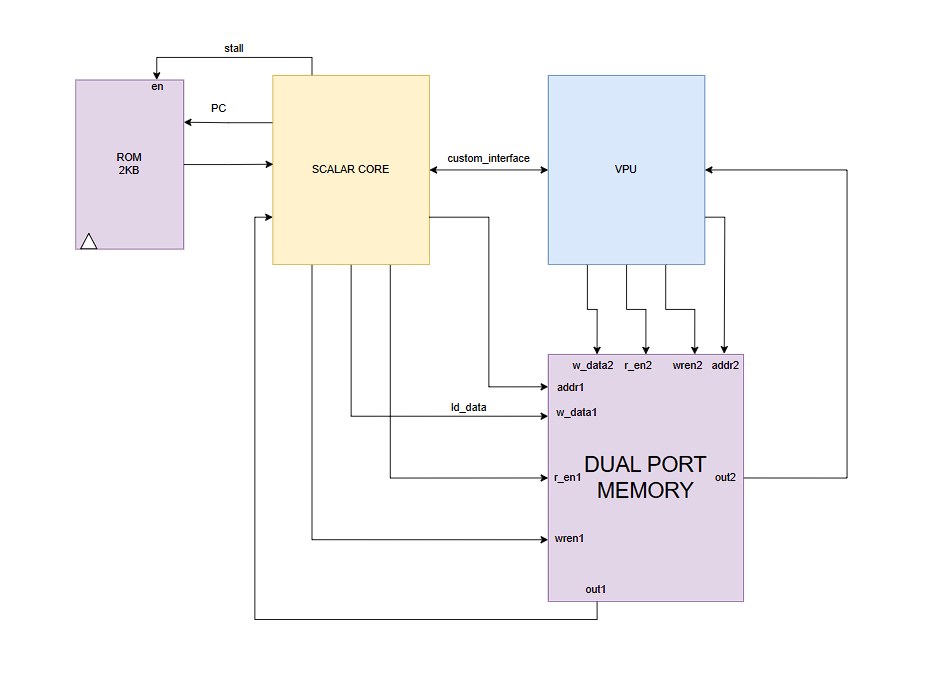
\includegraphics[width=\textwidth]{../image/harvard_architecture.png}
  \caption{Harvard memory architecture: IMEM connected to the IF stage (read-only),
           DMEM with dual scalar/VLSU ports connected to the MEM stage and vector LSU.}
  \label{fig:harvard_arch}
\end{figure}

\subsection{Instruction Memory (IMEM)}

The instruction memory is a synchronous single-port read-only memory with the
parameters shown in Table~\ref{tab:imem-spec}.

\begin{table}[H]
  \centering
  \caption{Instruction memory specification}
  \label{tab:imem-spec}
  \begin{tabular}{@{}ll@{}}
    \toprule
    \textbf{Parameter} & \textbf{Value} \\
    \midrule
    Base address          & \texttt{0x00000000} \\
    Size                  & 8~KB (2048 $\times$ 32-bit words) \\
    Access width          & 32 bits \\
    Latency               & 1 cycle (registered output) \\
    Contents              & \texttt{.text} and \texttt{.rodata} sections only \\
    Initialisation        & \texttt{\$readmemh} from \texttt{imem.hex} at simulation \\
    Write access          & None (read-only in hardware) \\
    \bottomrule
  \end{tabular}
\end{table}

The \texttt{imem.hex} file is generated from the compiled firmware ELF by the
\texttt{elf2hex\_lines.py} script, which converts the raw binary into one 32-bit
word per line in hexadecimal format. The linker script (\texttt{sw/link.ld}) places
\texttt{.text} at \texttt{0x00000000} and limits the total code size to 8~KB.

\subsection{Data Memory (DMEM)}

The data memory is a synchronous dual-port block RAM with the parameters shown in
Table~\ref{tab:dmem-spec}. Port~A services scalar load/store requests from the scalar
pipeline's MEM stage. Port~B services vector load/store requests from the VLSU.
Both ports can operate simultaneously, enabling the scalar and vector pipelines to
access memory in the same clock cycle without mutual stalling.

\begin{table}[H]
  \centering
  \caption{Data memory specification}
  \label{tab:dmem-spec}
  \begin{tabular}{@{}lll@{}}
    \toprule
    \textbf{Parameter} & \textbf{Port A (Scalar)} & \textbf{Port B (VLSU)} \\
    \midrule
    Base address   & \texttt{0x00000000} & \texttt{0x00000000} \\
    Size           & \multicolumn{2}{c}{64~KB (16384 $\times$ 32-bit words)} \\
    Access width   & 32 bits (byte-enable) & 32 bits (byte-enable) \\
    Latency        & 1 cycle              & 1 cycle \\
    Write support  & Yes                  & Yes (vector stores) \\
    Byte enable    & 4-bit mask           & 4-bit mask \\
    \bottomrule
  \end{tabular}
\end{table}

The VLSU uses \texttt{addr[15:2]} as the word index into the 64KB DMEM, consistent
with word-addressed access. Byte-enable signals allow sub-word writes for 8-bit and
16-bit vector element widths.

\subsection{Address Decode}

The scalar pipeline's LSU decodes memory addresses as follows:

\begin{itemize}
  \item \texttt{addr[31:8] == 24'h000000}: DMEM access (routed to Port~A of DMEM).
  \item \texttt{addr[31:8] == 24'hFF0000}: UART MMIO access (routed to UART TL-UL slave).
  \item All other addresses: undefined behaviour (no response, reads return zero).
\end{itemize}

The VLSU always accesses DMEM via Port~B regardless of the address, since vector
data is guaranteed by the firmware to reside in the DMEM range.

\section{UART Interface Specification}
\label{sec:uart-spec}

\subsection{Physical Framing}

The UART interface uses the 8-N-1 framing format: one start bit (logic 0), eight data
bits (LSB first), no parity bit, and one stop bit (logic 1). The baud rate is
configurable via RTL parameters but defaults to 115200~baud for production firmware.

At 115200~baud, the bit period is $1/115200 \approx 8.68~\mu$s. The UART baud clock
is derived by dividing the system clock by a baud divisor:
\begin{equation}
  \text{baud\_div} = \left\lfloor \frac{f_\text{clk}}{\text{baud\_rate}} \right\rfloor
  \label{eq:baud-div}
\end{equation}
For the simulation default of $f_\text{clk} = 14.7456~\text{MHz}$, baud\_div=128,
giving 128 clock cycles per bit. For the FPGA default of $f_\text{clk} = 50~\text{MHz}$,
baud\_div=434.

\subsection{MMIO Register Map}

The UART is mapped as a TileLink Uncached Lightweight (\gls{tlu}) slave at base address
\texttt{0xFF000000}. Table~\ref{tab:uart-regs} shows the register map.

\begin{table}[H]
  \centering
  \caption{UART MMIO register map}
  \label{tab:uart-regs}
  \begin{tabular}{@{}llll@{}}
    \toprule
    \textbf{Offset} & \textbf{Register} & \textbf{Access} & \textbf{Description} \\
    \midrule
    \texttt{+0x00} & CTRL   & RW & Control register (reserved for future use) \\
    \texttt{+0x04} & STAT   & RO & Status register \\
    \texttt{+0x08} & TXDAT  & WO & Transmit data register \\
    \texttt{+0x0C} & RXDAT  & RO & Receive data register \\
    \bottomrule
  \end{tabular}
\end{table}

\subsubsection{STAT Register (offset +0x04)}

\begin{table}[H]
  \centering
  \caption{UART STAT register bit assignments}
  \label{tab:uart-stat}
  \begin{tabular}{@{}cll@{}}
    \toprule
    \textbf{Bit} & \textbf{Field} & \textbf{Description} \\
    \midrule
    \texttt{[0]} & \texttt{tx\_ready} & 1 = TX shift register is empty, ready for new byte \\
    \texttt{[1]} & \texttt{rx\_valid} & 1 = RX FIFO contains at least one byte \\
    \texttt{[31:2]} & ---            & Reserved, read as zero \\
    \bottomrule
  \end{tabular}
\end{table}

\subsubsection{TXDAT Register (offset +0x08)}

Writing a byte to this register loads it into the transmit shift register. Writes are
ignored if \texttt{tx\_ready} is 0. Firmware must poll \texttt{tx\_ready} in the STAT
register before each write to avoid dropping characters.

\subsubsection{RXDAT Register (offset +0x0C)}

Reading this register returns the oldest byte in the receive FIFO in bits [7:0].
Bits [31:8] read as zero. If \texttt{rx\_valid} is 0, the read returns an undefined
value. Firmware must poll \texttt{rx\_valid} in the STAT register before each read.

\subsection{Firmware Programming Model}

A typical firmware receive-byte function polls the STAT register until \texttt{rx\_valid}
is set, then reads RXDAT:

\begin{lstlisting}[language=RISCV, caption={UART receive byte (polling)}]
# a0 = UART base address (0xFF000000)
# Returns received byte in a0
uart_getchar:
    li   t0, 0xFF000000   # UART base
.wait_rx:
    lw   t1, 4(t0)        # read STAT
    andi t1, t1, 2        # test rx_valid bit
    beqz t1, .wait_rx     # spin until byte available
    lw   a0, 12(t0)       # read RXDAT
    andi a0, a0, 0xFF     # mask to 8 bits
    ret
\end{lstlisting}

\begin{lstlisting}[language=RISCV, caption={UART transmit byte (polling)}]
# a0 = byte to transmit
# Uses t0--t1 as temporaries
uart_putchar:
    li   t0, 0xFF000000   # UART base
.wait_tx:
    lw   t1, 4(t0)        # read STAT
    andi t1, t1, 1        # test tx_ready bit
    beqz t1, .wait_tx     # spin until TX ready
    sw   a0, 8(t0)        # write TXDAT
    ret
\end{lstlisting}

\subsection{Timing Constraints}

The UART's TL-UL slave interface is registered: the channel-D response to a channel-A
request is registered at the output, introducing a one-cycle read latency. This matches
the one-cycle latency of the DMEM, ensuring that the scalar pipeline's load path has
the same timing whether accessing DMEM or the UART.

For synthesis, the UART datapath must meet setup timing at the target clock frequency.
The baud divisor counter is a simple 16-bit counter; its path from counter register
to the baud-clock enable is not on the critical path. The TL-UL address comparator
(checking \texttt{addr[31:8] == 24'hFF0000}) adds one level of logic to the address
decode path, which is accounted for in the FPGA timing analysis.

\section{Performance Requirements}
\label{sec:perf-requirements}

\subsection{Target Clock Frequency}

The design shall achieve a minimum $F_\text{max}$ of 50~MHz on the Intel Cyclone~V
(5CSXFC6D6F31C8) device used on the DE10-Standard board \cite{de10standard}. This
target is chosen to enable real-time processing of a 640$\times$480 video frame
at approximately 2~frames per second with the single-lane architecture, providing
a meaningful demonstration of the vector processing capability.

At 50~MHz with VLEN=128, SEW=8, and LMUL=1 (16 elements per cycle), the VLSU achieves
a data throughput of:
\begin{equation}
  \text{Throughput}_\text{load} = 50 \times 10^6 \text{ Hz} \times \frac{4~\text{bytes}}{\text{cycle}} = 200~\text{MB/s}
  \label{eq:load-throughput}
\end{equation}
for unit-stride loads (one 32-bit word per cycle from DMEM).

For arithmetic throughput at SEW=8, the single-lane processes 4 elements per 32-bit
lane per cycle when the cycle counter advances, giving 4~Gops/s at 1~GHz or 200~Mops/s
at 50~MHz. The BT.601 grayscale benchmark requires $3 \times 16384 = 49152$ multiply
operations and 16384 additions for the luminance channel of a 128$\times$128 image;
at 200~Mops/s this completes in approximately 0.33~ms.

\subsection{Area Budget}

The target area budget for FPGA prototyping is 12000~\glspl{alm} on the Cyclone~V
device. This leaves sufficient resources for debugging logic, block RAM, and any
future additions. The measured area after synthesis and place-and-route is 10438~ALMs,
confirming that the implementation meets this budget with approximately 13\% headroom.

For a future ASIC implementation in a 28nm or 22nm technology node, an informal
estimate based on the ALM count and typical ALM-to-gate ratios suggests a target
of 50000--100000 standard-cell gate equivalents for the core logic, excluding
memory macros.

\subsection{Power Estimation}

Quantitative power estimates for the FPGA prototype are not the primary deliverable
of this thesis; the FPGA fabric's configurable routing introduces significant static
power overhead that is not representative of an ASIC implementation. However, the
design incorporates clock-gating enable signals (\texttt{vrf\_wren}, \texttt{*\_en})
on the vector register file and LSU data-path registers so that power estimation tools
in a future ASIC flow can infer clock gating cells at these control points, meeting
the ASIC design rule requiring explicit enable signals on all high-fan-out registers.

\chapter{Hardware Design}
\label{ch:hardware}

This chapter presents the complete microarchitectural design of the \gls{riscv} \gls{vpu}
system. The design implements the \texttt{rv32im\_zicsr\_zve32x\_zvl128b} instruction
set, targeting \gls{asic} tapeout with VLEN~=~128 bits. Every design decision is motivated
by synthesisability, timing closure at the target frequency, and area economy.
The chapter proceeds from the top-level integration, through the scalar pipeline, into
the \gls{vpu} subsystem and its constituent functional units, and concludes with the
memory subsystem and \gls{uart} peripheral.

%% =============================================================================
\section{System Architecture Overview}
\label{sec:system_arch}
%% =============================================================================

\subsection{Top-Level Integration}
\label{subsec:toplevel}

The top-level module \texttt{riscv\_vpu\_top\_v4} integrates five major subsystems on a
common clock domain: the five-stage scalar pipeline (\texttt{pipelined\_vpu}), the
\gls{vpu} subsystem (\texttt{vproc\_system\_wrapper}), a synchronous dual-port data
memory (\texttt{dmem\_sync}), a synchronous instruction memory (\texttt{imem\_sync}),
and a \gls{uart} controller. The module is parameterised by \texttt{CLK\_FREQ} and
\texttt{BAUD\_RATE} so that simulations may run at a high baud divisor without modifying
firmware; the default configuration uses $\mathit{CLK\_FREQ} = 14{,}745{,}600$~Hz and
$\mathit{BAUD\_RATE} = 115{,}200$~baud, yielding a divisor of 128.

\begin{figure}[H]
  \centering
  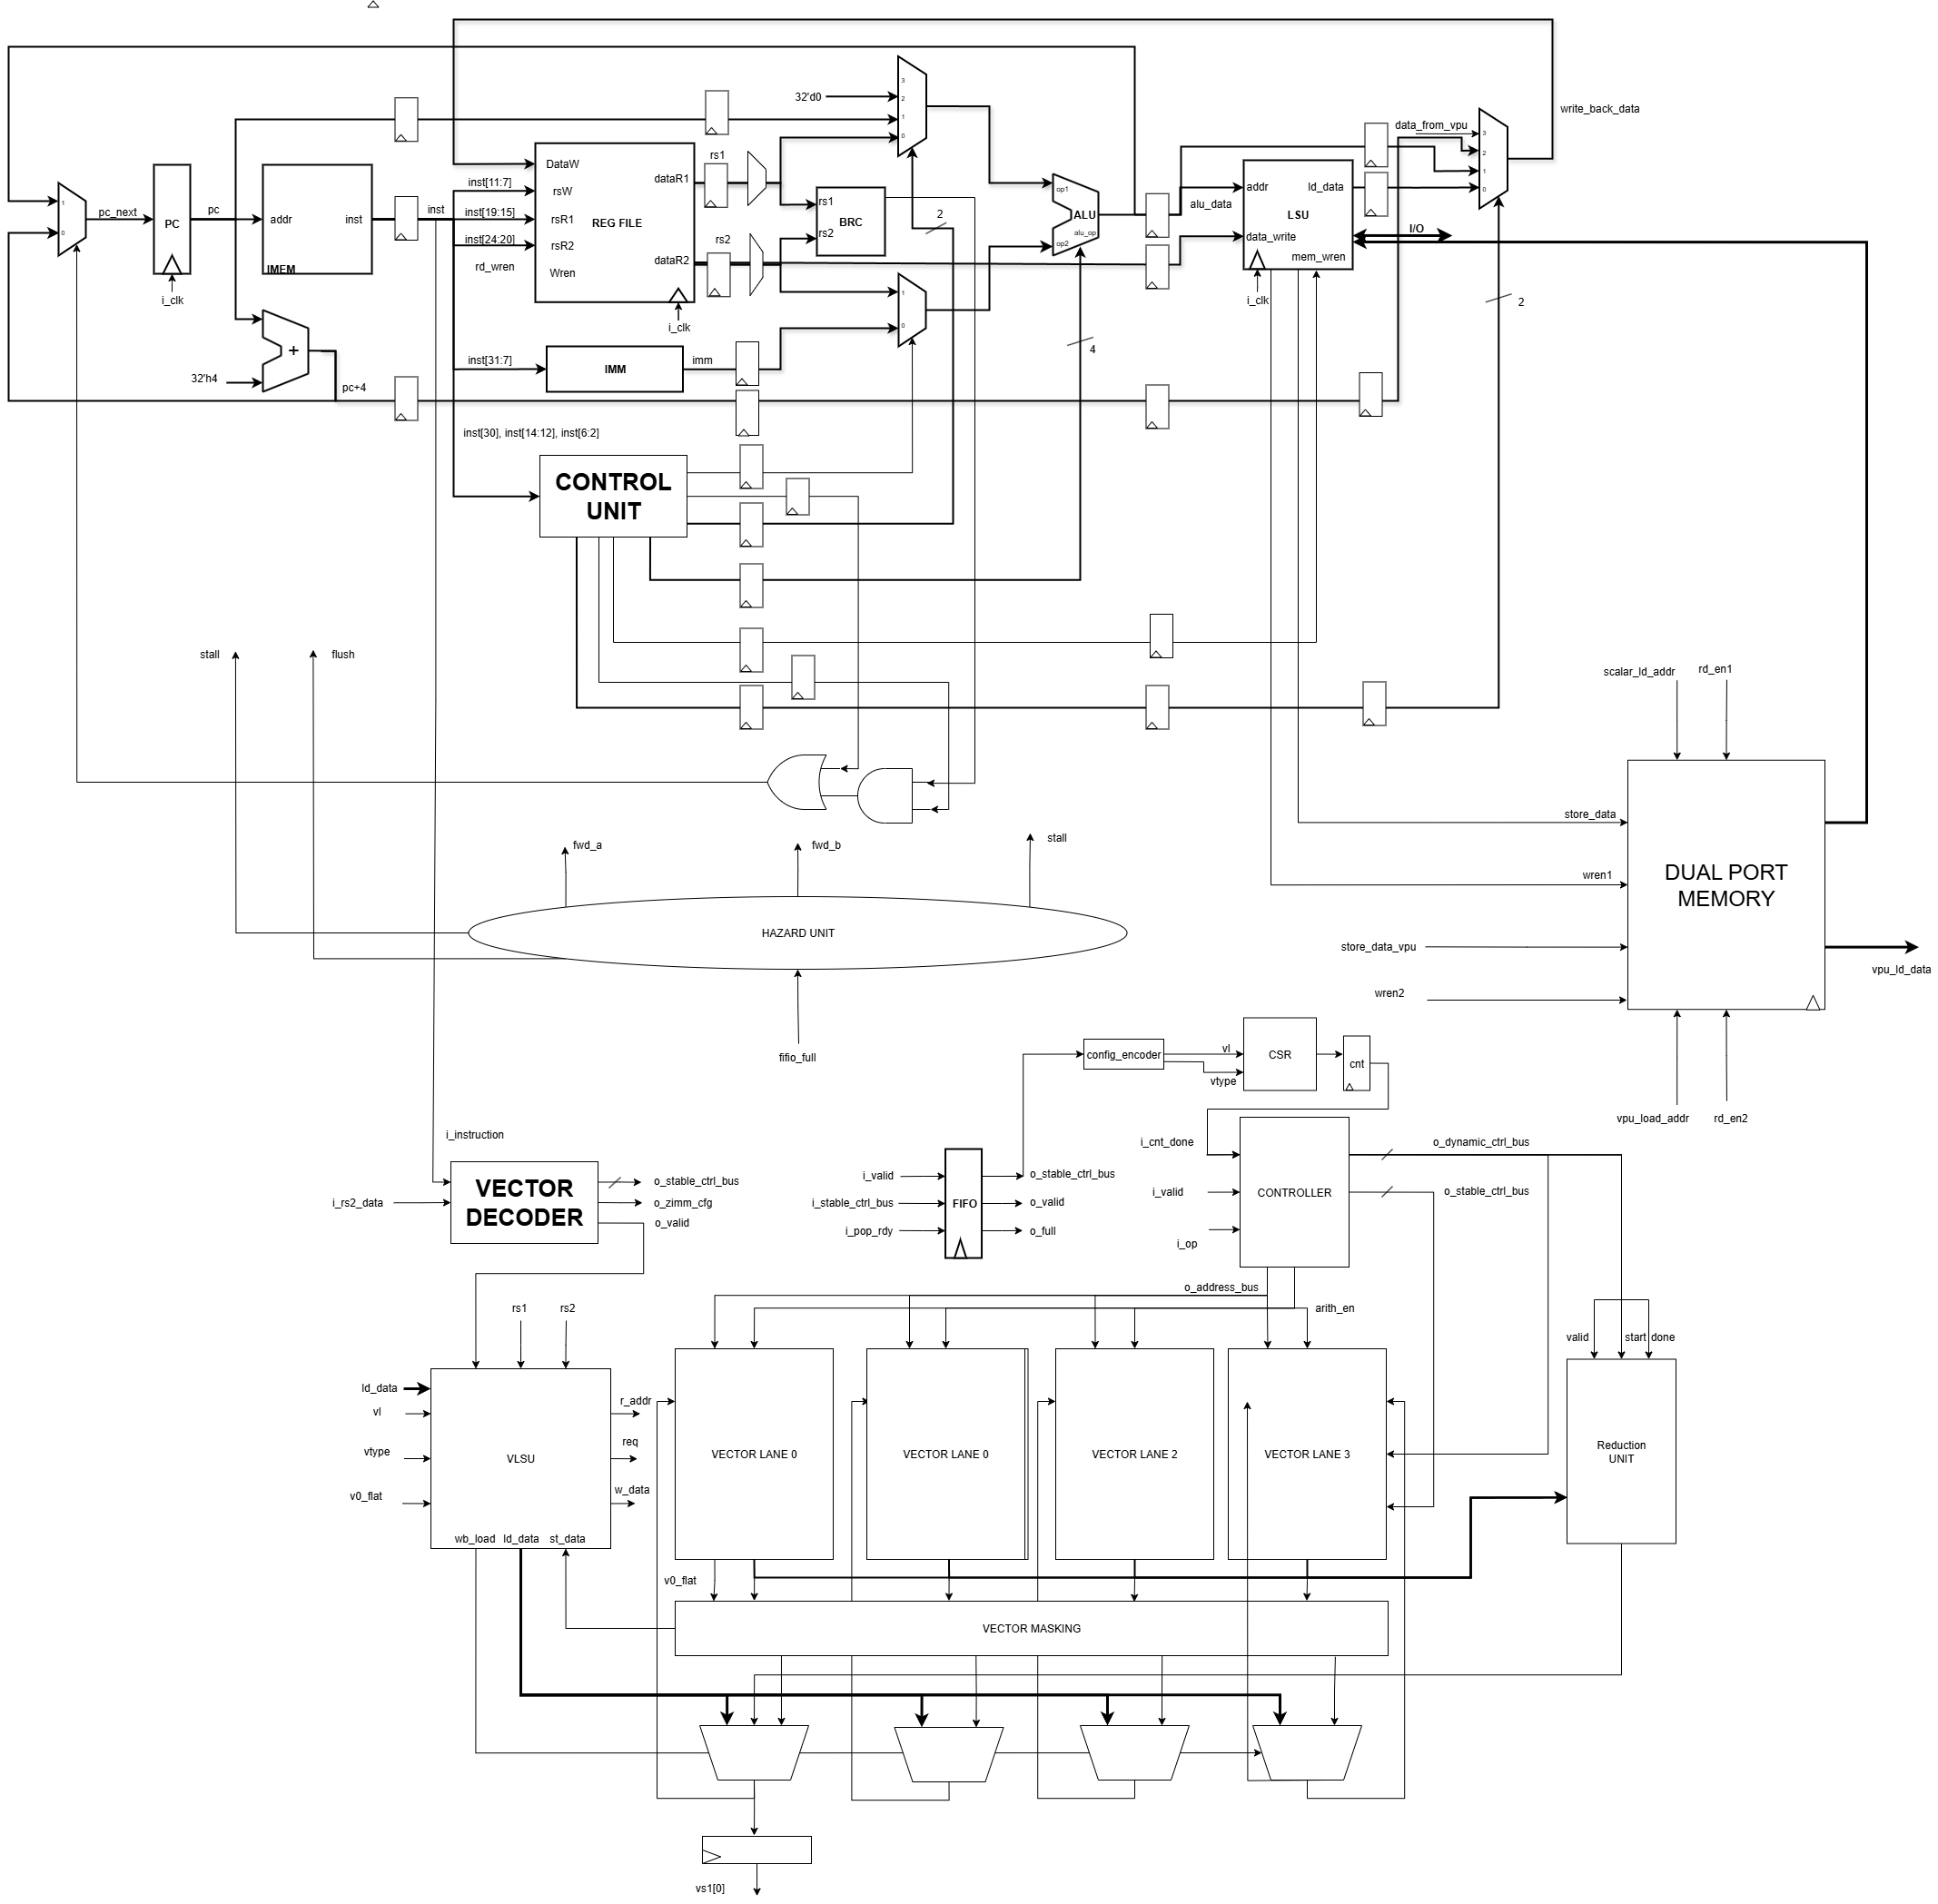
\includegraphics[width=\textwidth]{../image/TOP_design.png}
  \caption{Top-level block diagram of \texttt{riscv\_vpu\_top}: scalar pipeline,
           VPU subsystem, IMEM, DMEM (dual-port), and interconnect buses.}
  \label{fig:top_design}
\end{figure}

Address decoding is performed inline without a bus arbiter. The scalar core presents
a 32-bit byte address on its DMEM port. A single combinational comparator checks
whether bits~[31:8] equal \texttt{0xFF0000}; if so, the transaction is steered to the
\gls{uart} TL-UL interface; otherwise it reaches \texttt{dmem\_sync} port~A. This
approach keeps the critical path short and eliminates the area overhead of a full
interconnect fabric, which is appropriate for a single-master system.

\subsection{Clock and Reset Distribution}
\label{subsec:clk_reset}

A single clock, \texttt{i\_clk}, is used throughout the design. The external reset pin
\texttt{i\_reset} is active-high for compatibility with FPGA push-button convention;
it is immediately inverted to \texttt{rst\_n} (active-low) at the top level so that
every submodule sees the \gls{asic}-standard active-low synchronous reset interface.
All flip-flops in \texttt{vproc\_system\_wrapper} and \texttt{vproc\_vec\_lsu} use
\texttt{posedge clk / negedge rst\_n}, producing synthesisable reset trees. The scalar
pipeline registers use synchronous active-high reset (\texttt{i\_reset}) directly,
following the convention established in the \gls{riscv} scalar core.

No clock gating cells are instantiated explicitly in RTL; clock enable signals
(\texttt{write\_en[3:0]} on the \gls{vrf}, pipeline stall enables, and VLSU advance
conditions) are present on every register bank to allow automatic clock-gating
inference by a downstream synthesis tool. The power-reduction benefit is most
significant on the \gls{vrf} banks, which collectively hold $32 \times 4 \times
8 = 1024$ flip-flops, and would otherwise toggle unnecessarily on every cycle.

\subsection{Signal Interface Summary}
\label{subsec:sig_table}

\begin{table}[H]
\centering
\caption{Top-level inter-subsystem buses and their widths}
\label{tab:top_buses}
\begin{tabular}{llcl}
\toprule
\textbf{Bus / Signal Group} & \textbf{Direction} & \textbf{Width (bits)} & \textbf{Description} \\
\midrule
\texttt{PC} (scalar $\to$ IMEM)               & Scalar $\to$ IMEM   & 32  & Word-aligned program counter \\
\texttt{instr} (IMEM $\to$ scalar)            & IMEM $\to$ Scalar   & 32  & Registered instruction word \\
Scalar DMEM port A (addr/wdata/rdata/we/be/re) & Scalar $\leftrightarrow$ DMEM & 32+32+32+1+4+1 & Scalar load/store \\
VLSU DMEM port B (addr/wdata/rdata/req/we/be/ready) & VPU $\leftrightarrow$ DMEM & 32+32+32+1+1+4+1 & Vector load/store \\
\texttt{vpu\_insn\_vld}                        & Scalar $\to$ VPU    & 1   & OP-V instruction valid \\
\texttt{vpu\_insn}                             & Scalar $\to$ VPU    & 32  & Dispatched instruction \\
\texttt{vpu\_rs1\_data}, \texttt{vpu\_rs2\_data} & Scalar $\to$ VPU  & 32  & Scalar register operands \\
\texttt{vpu\_ready}                            & VPU $\to$ Scalar    & 1   & Back-pressure: 0 = stall scalar \\
\texttt{vpu\_cfg\_done}                        & VPU $\to$ Scalar    & 1   & \texttt{vsetvl*} commit pulse \\
\texttt{vpu\_vl\_remain}                       & VPU $\to$ Scalar    & 32  & New \texttt{vl} for scalar \texttt{rd} writeback \\
TL-UL A channel (\texttt{uart\_tl\_a})         & Scalar $\to$ UART   & 71  & TL-UL A-channel bundle \\
TL-UL D channel (\texttt{uart\_tl\_d})         & UART $\to$ Scalar   & 33  & TL-UL D-channel bundle \\
\texttt{uart\_rx}, \texttt{uart\_tx}            & External I/O        & 1 each & Serial data lines \\
\bottomrule
\end{tabular}
\end{table}

%% =============================================================================
\section{Scalar RISC-V Core}
\label{sec:scalar_core}
%% =============================================================================

The scalar core implements the \texttt{rv32im\_zicsr} subset as a classical five-stage
in-order pipeline: Instruction Fetch (IF), Instruction Decode (ID), Execute (EX),
Memory (MEM), and Write-Back (WB). The design is contained in the
\texttt{pipelined\_vpu} module and uses synchronous active-high reset internally.

\subsection{Pipeline Structure}
\label{subsec:pipeline_structure}

\begin{figure}[H]
  \centering
  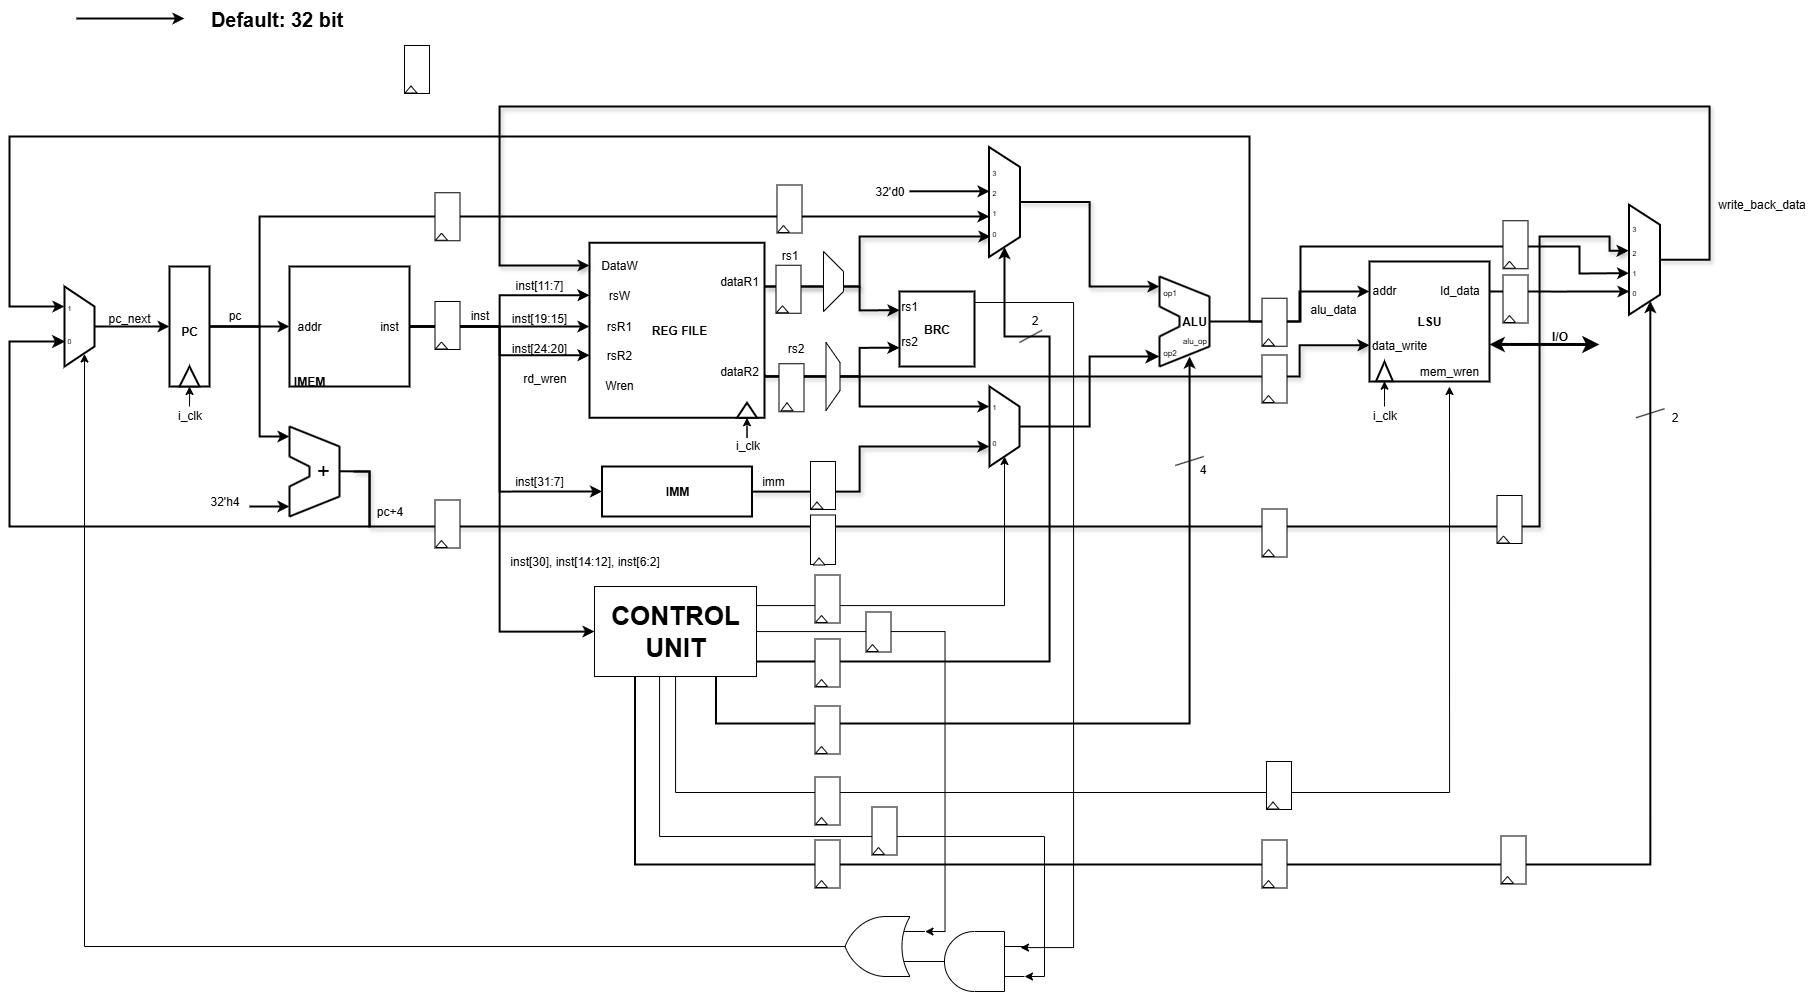
\includegraphics[width=\textwidth]{../image/Top-level_block_diagram.png}
  \caption{Five-stage scalar pipeline datapath of \texttt{pipelined\_vpu}}
  \label{fig:pipeline_datapath}
\end{figure}

\textbf{Instruction Fetch (IF).} The program counter \texttt{pc} is a 32-bit
synchronous register that resets to zero. It advances by 4 each cycle unless a stall
or branch-taken condition is asserted. Instruction memory (\texttt{imem\_sync}) is a
synchronous SRAM with a one-cycle read latency; the registered output arrives directly
at the ID stage, eliminating a redundant IF/ID instruction register. On a branch taken
or jump (\texttt{pc\_sel}), the IF stage is flushed by injecting a NOP
(\texttt{32'h0000\_0013}, \texttt{ADDI x0,x0,0}) into \texttt{imem\_sync}'s output
register.

\textbf{Instruction Decode (ID).} The control unit decodes the 11-bit pattern
\texttt{\{instr[30], instr[14:12], instr[6:0]\}} and generates the full set of control
signals: \texttt{br\_ctrl}, \texttt{j\_taken}, \texttt{ImmSel}, \texttt{alu\_op},
\texttt{wb\_sel}, \texttt{mem\_wren}, \texttt{rd\_wren}, \texttt{is\_load}, and
\texttt{is\_vector}. The register file is read combinatorially; two bypass muxes
(\texttt{rf1\_fwd}, \texttt{rf2\_fwd}) apply the WB result to the register-file output
in the same cycle to avoid a write-before-read race.

\textbf{Execute (EX).} The ALU computes the result using a 4-bit opcode
(\texttt{alu\_op\_exe}). Operand-A is selected between \texttt{rs1\_data} (forwarded)
and the EX-stage PC (\texttt{pce}) via \texttt{opa\_sel\_exe}; operand-B is selected
between forwarded \texttt{rs2\_data} and the sign-extended immediate via
\texttt{opb\_sel\_exe}. A separate branch comparator (\texttt{brc}) evaluates the
branch condition using the forwarded operands without consuming the ALU.

\textbf{Memory (MEM).} Load and store instructions access \texttt{dmem\_sync} through
the scalar port. The IO region (\texttt{addr[31:16] == 0x1000}) is handled inline:
writes update local registers (\texttt{ledr\_r}, \texttt{ledg\_r}, etc.); reads return
the corresponding register values. UART-mapped addresses (\texttt{addr[31:8] == 0xFF0000})
are decoded at the top level and steered away from \texttt{dmem\_sync}.

\textbf{Write-Back (WB).} A 2-bit selector \texttt{wb\_sel\_wb} chooses between load
data (0), ALU result (1), PC+4 (2), or immediate (3). Load-data sign and zero extension
is computed combinatorially based on \texttt{func3\_wb} and the low-order address bits
\texttt{addr\_lo\_wb}. Byte and half-word loads are supported (\texttt{LB}, \texttt{LH},
\texttt{LBU}, \texttt{LHU}).

\subsection{Hazard Detection}
\label{subsec:hazard}

Two independent hazard conditions require pipeline stalls or flushes.

\textbf{Load-use hazard.} When a load instruction (\texttt{is\_load\_exe = 1}) is in
the EX stage and the immediately following instruction in ID reads the same destination
register, the result is not available for forwarding in time. The detection condition is:

\begin{equation}
\mathit{stall\_ld} = \mathit{is\_load\_exe} \;\wedge\; (\mathit{rd\_exe} \neq \mathbf{0})
  \;\wedge\; (\mathit{rd\_exe} = \mathit{rs1_{ID}} \;\vee\; \mathit{rd\_exe} = \mathit{rs2_{ID}})
\label{eq:load_use}
\end{equation}

When \texttt{stall\_ld} is asserted, the PC register and IF/ID pipeline registers are
held (\texttt{stall = 1}) and a bubble is injected into the ID/EX registers by
zeroing all control signals in the \texttt{hazard} path.

\textbf{VPU dispatch stall.} When a vector instruction reaches the EX stage
(\texttt{is\_vector\_exe = 1}) and the \gls{vpu} signals it is not ready
(\texttt{vpu\_ready\_i = 0}), the entire pipeline is held:

\begin{equation}
\mathit{vpu\_stall} = \mathit{is\_vector\_exe} \;\wedge\; \neg\,\mathit{vpu\_ready\_i}
\label{eq:vpu_stall}
\end{equation}

All pipeline registers from PC through MEM/WB are clock-enabled with
\texttt{!vpu\_stall}, so the entire pipeline freezes until \texttt{vpu\_ready\_i} goes
high. This simple freeze-and-hold approach is correct because the vector instruction
itself is already in the EX stage driving \texttt{vpu\_insn\_o} and \texttt{vpu\_rs1/rs2\_data\_o};
the \gls{vpu} latches these on the first cycle that \texttt{vpu\_ready} is high.

\subsection{Data Forwarding}
\label{subsec:forwarding}

Full EX$\to$MEM and MEM$\to$WB forwarding bypasses are implemented to avoid
unnecessary stalls for back-to-back ALU instructions. The forwarding priority for
operand A of the EX stage is:

\begin{enumerate}
  \item \texttt{fwd\_a = 2'b01}: Forward from EX/MEM register (\texttt{alu\_result\_m})
        when the MEM-stage instruction writes the same register as rs1 in EX.
  \item \texttt{fwd\_a = 2'b10}: Forward from the WB writeback path (\texttt{rf\_wdata})
        when the WB-stage instruction writes rs1 in EX.
  \item \texttt{fwd\_a = 2'b00}: Use the ID/EX register value directly.
\end{enumerate}

The same priority chain applies to operand B (\texttt{fwd\_b}). Forwarding from
\texttt{rf\_wdata} rather than the MEM/WB register output is intentional: it picks up
VPU configuration writebacks (Section~\ref{subsec:vpu_dispatch}) transparently.

\subsection{VPU Dispatch Protocol}
\label{subsec:vpu_dispatch}

When the control unit decodes an OP-V opcode (\texttt{is\_vector = 1}), the instruction
propagates to the EX stage in the normal fashion. In the EX stage, the core continuously
drives \texttt{vpu\_insn\_vld\_o = is\_vector\_exe} and presents the instruction word
plus forwarded operands on \texttt{vpu\_insn\_o}, \texttt{vpu\_rs1\_data\_o}, and
\texttt{vpu\_rs2\_data\_o}.

The \gls{vpu} accepts the instruction when it asserts \texttt{vpu\_ready}; simultaneously,
the scalar pipeline resumes. If the \gls{vpu} deasserts \texttt{vpu\_ready} (FIFO full
or \gls{vlsu} busy), the pipeline stalls via \texttt{vpu\_stall} until acceptance.

A special case applies to \texttt{vsetvl}/\texttt{vsetvli} instructions
(\texttt{is\_cfg\_exe}). These must write the new \texttt{vl} value back to a scalar
general-purpose register (\texttt{rd}). Because the \gls{vpu} updates its internal CSR
asynchronously over several cycles, the scalar core captures the destination register
address (\texttt{rd\_addr\_exe}) in a pending register (\texttt{vpu\_cfg\_rd\_r}) and
waits for the \texttt{vpu\_cfg\_done\_i} pulse. When \texttt{vpu\_cfg\_done\_i} arrives,
the RF write port is overridden:

\begin{lstlisting}[language=SV, caption={VPU config writeback in WB stage},
                   label={lst:cfg_wb}]
always_comb begin
    if (vpu_cfg_done_i && vpu_cfg_pending_r && vpu_cfg_rd_r != 5'b0) begin
        rf_wren  = 1'b1;
        rf_waddr = vpu_cfg_rd_r;
        rf_wdata = vpu_vl_remain_i; // actual vl from VPU CSR
    end else begin
        rf_wren  = rd_wren_wb;
        rf_waddr = rd_addr_wb;
        rf_wdata = wb_data;
    end
end
\end{lstlisting}

%% =============================================================================
\section{VPU Architecture}
\label{sec:vpu_arch}
%% =============================================================================

The \gls{vpu} subsystem is contained within \texttt{vproc\_system\_wrapper}, which
instantiates the decoder, FIFO, FSM, cycle counter, four \gls{vrf} banks, four
processor lanes, the reduction unit, the vector \gls{vlsu}, and auxiliary units
(address generator, CSR, mask enable, mask write buffer, merge unit, scalar expand).
The entire subsystem is parameterised by \texttt{NUM\_REGS}~=~32, \texttt{ADDR\_WIDTH}~=~5,
and \texttt{CTRL\_WIDTH}~=~49 (the 48-bit logical bus plus a \texttt{vsetivli} flag).

\begin{figure}[H]
  \centering
  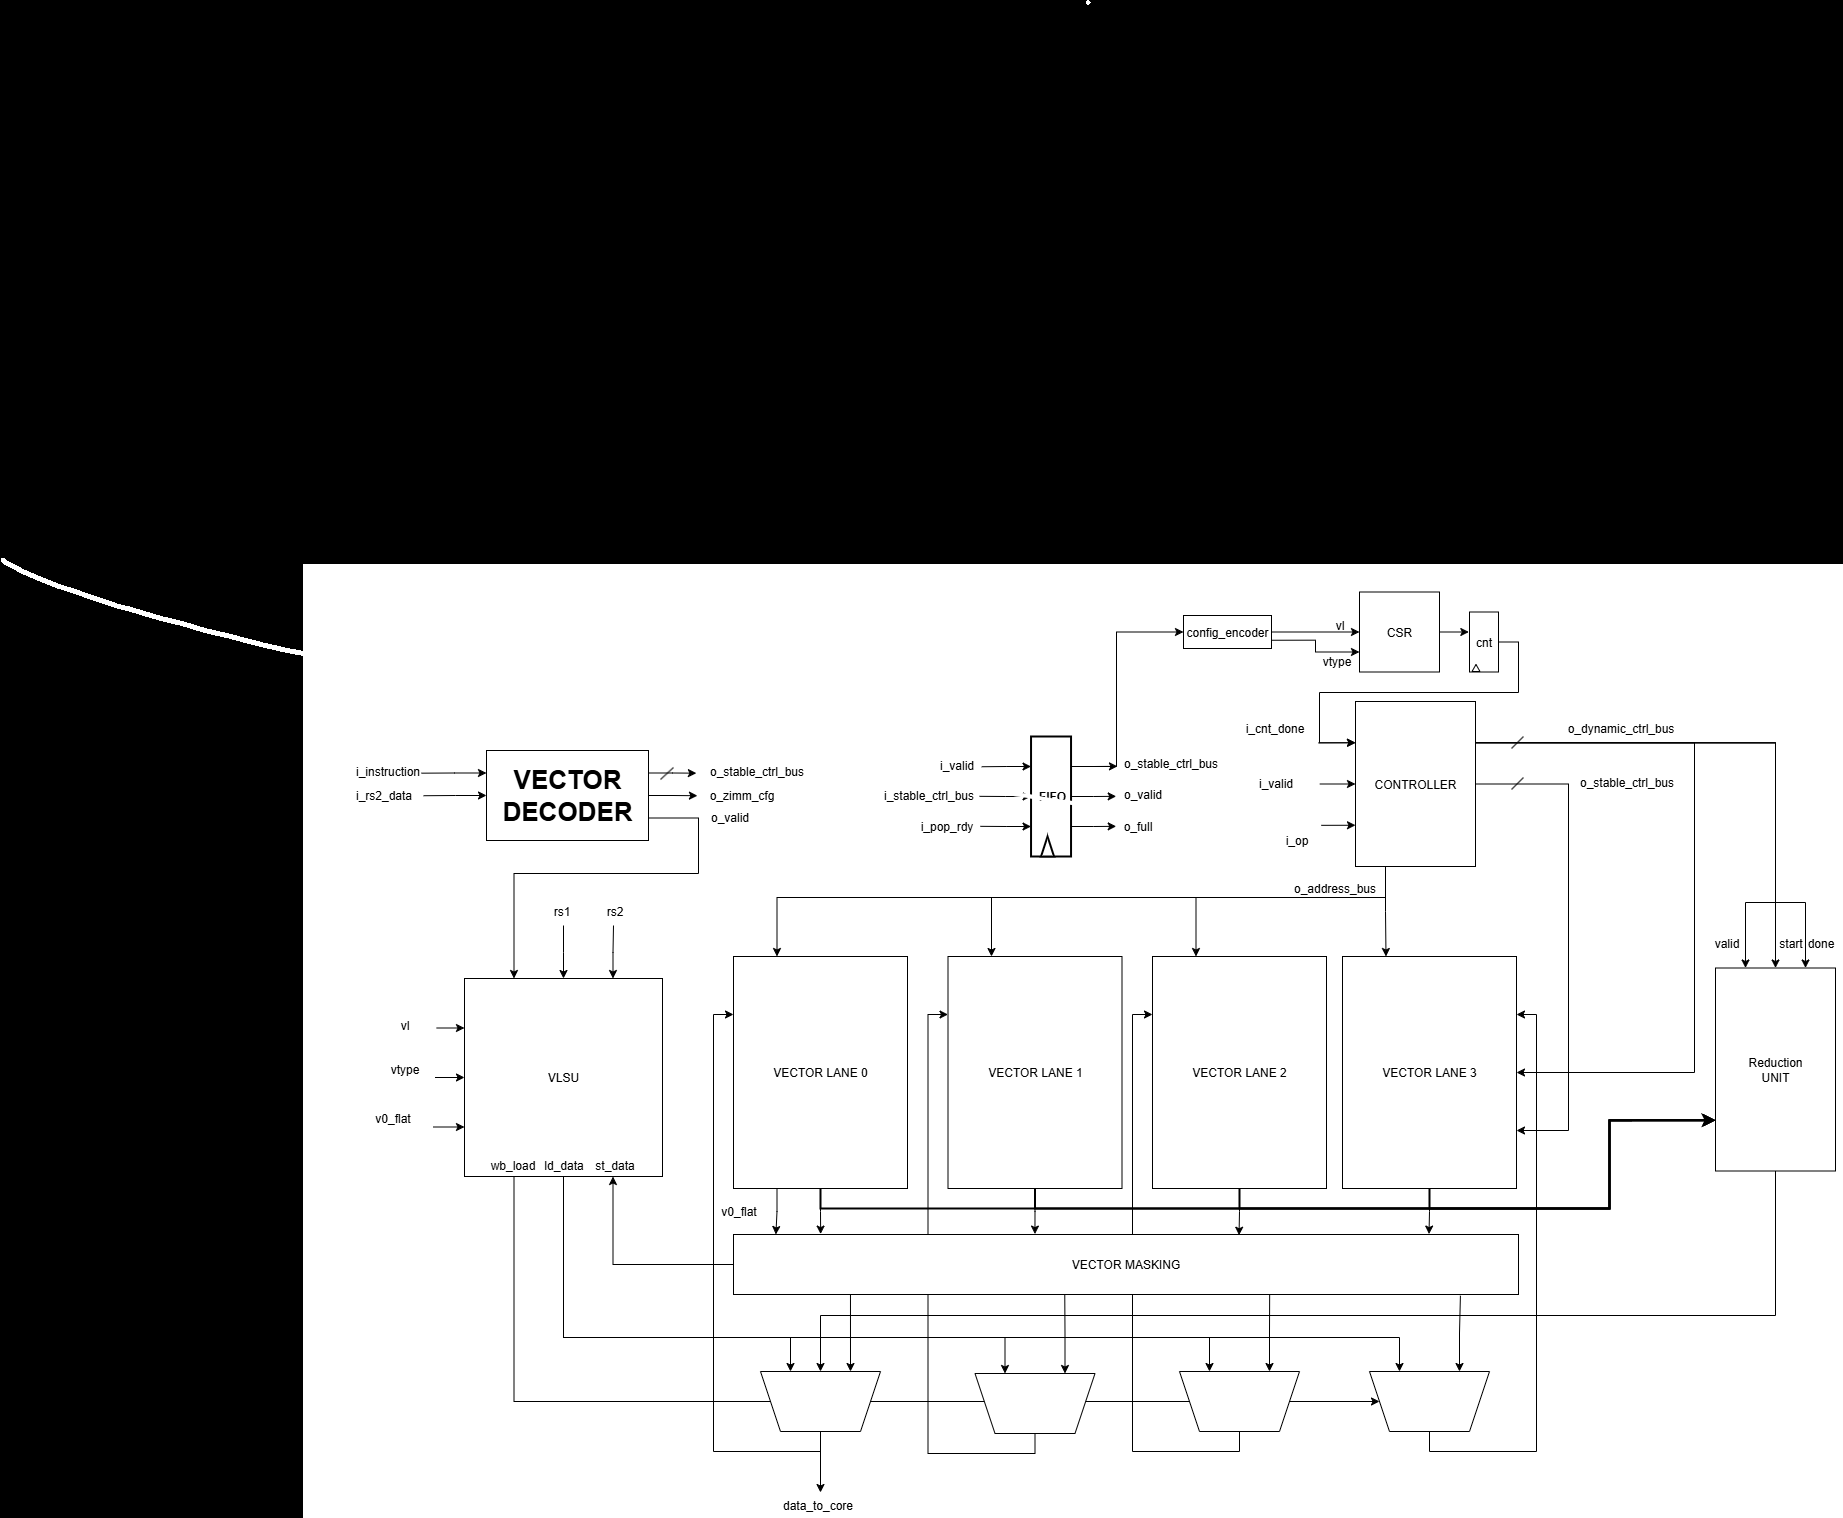
\includegraphics[width=\textwidth]{../image/vpu_top_wrapper.png}
  \caption{Block diagram of the \texttt{vproc\_system\_wrapper} VPU subsystem}
  \label{fig:vpu_wrapper}
\end{figure}

\subsection{Instruction Decoder}
\label{subsec:decoder}

The decoder module \texttt{vproc\_vdecoder} accepts a 32-bit RVV instruction word and
produces a 49-bit \texttt{ctrl\_bus} that encodes all execution control fields. The
decoding is purely combinational; the decoder also outputs a 32-bit sign-extended
immediate for \texttt{vimm*} instructions.

\subsubsection{ctrl\_bus Layout}

\begin{table}[H]
\centering
\caption{49-bit \texttt{ctrl\_bus} field encoding}
\label{tab:ctrlbus}
\begin{tabular}{clp{7cm}}
\toprule
\textbf{Bits} & \textbf{Field} & \textbf{Meaning} \\
\midrule
{[4:0]}   & \texttt{vs1\_addr}          & Source register 1 address (5-bit) \\
{[9:5]}   & \texttt{vs2\_addr}          & Source register 2 address \\
{[14:10]} & \texttt{vd\_addr}           & Destination register address \\
{[20:15]} & \texttt{funct6}             & Instruction funct6 field \\
{[21]}    & \texttt{is\_widen}          & Widening operation (result is 2$\times$ SEW) \\
{[22]}    & \texttt{is\_unsigned\_vs1}  & vs1 treated as unsigned \\
{[23]}    & \texttt{is\_unsigned\_vs2}  & vs2 treated as unsigned \\
{[24]}    & \texttt{is\_subtraction}    & Negate adder (vsub/vrsub) \\
{[25]}    & \texttt{is\_immediate}      & Use zimm/imm operand instead of vs1 \\
{[26]}    & \texttt{is\_rs1}            & Use scalar rs1 as vs1 \\
{[27]}    & \texttt{is\_mulh}           & Select upper-half multiplier product \\
{[28]}    & \texttt{is\_config}         & vsetvl/vsetvli instruction \\
{[29]}    & \texttt{is\_vector}         & OP-V opcode family \\
{[30]}    & \texttt{cfg\_is\_vsetvli}   & 1 = vsetvli, 0 = vsetvl \\
{[31]}    & \texttt{vm}                 & Mask bit from instruction [25]: 1 = unmasked \\
{[39:32]} & \texttt{vtype\_enc}         & \texttt{\{vma,vta,vsew[2:0],vlmul[2:0]\}} \\
{[40]}    & \texttt{is\_carry}          & vadc/vsbc with carry from v0 \\
{[41]}    & \texttt{is\_mask\_carry}    & vmadc/vmsbc — result is a carry mask \\
{[42]}    & \texttt{is\_masking}        & Mask-generating instruction (vmseq, etc.) \\
{[43]}    & \texttt{is\_final\_masking} & Requires ST\_FINAL\_MASKING commit phase \\
{[44]}    & \texttt{is\_reverse\_sub}   & vrsub: swap minuend/subtrahend \\
{[45]}    & \texttt{minmax\_is\_min}    & 1 = vmin/vminu; 0 = vmax/vmaxu \\
{[46]}    & \texttt{minmax\_is\_unsign} & 1 = unsigned comparison for min/max \\
{[47]}    & \texttt{is\_reduction}      & vred* instruction \\
{[48]}    & \texttt{cfg\_is\_vsetivli}  & 1 = vsetivli (AVL from 5-bit immediate) \\
\bottomrule
\end{tabular}
\end{table}

\subsubsection{Decoding Categories}

The decoder classifies every instruction into one of five execution categories, which
determine the \gls{fsm} state sequence:

\begin{description}
  \item[Config (\texttt{is\_config}).] Instructions \texttt{vsetvl}, \texttt{vsetvli},
    and \texttt{vsetivli} update the CSR registers \texttt{vl} and \texttt{vtype}.
    No \gls{vrf} access occurs; the \gls{fsm} traverses ST\_IDLE $\to$ ST\_CONFIG $\to$
    ST\_IDLE in a single cycle.
  \item[Masking (\texttt{is\_masking}).] Instructions such as \texttt{vmseq.vv},
    \texttt{vmslt.vv}, and \texttt{vmadc.vv} produce a 1-bit result per element that
    is packed into a destination mask register. The \gls{fsm} accumulates comparison
    bits over multiple cycles (ST\_MASKING) then writes the complete packed result in
    one cycle (ST\_FINAL\_MASKING).
  \item[Widening (\texttt{is\_widen}).] Two-cycle widening instructions (e.g.,
    \texttt{vaddw.vv}) alternate between ST\_WIDENL (write low half) and ST\_WIDENH
    (write high half) until all elements are processed.
  \item[Reduction (\texttt{is\_reduction}).] Instructions \texttt{vredsum.vs},
    \texttt{vredmax.vs}, etc. use the dedicated reduction unit in a serial
    accumulation loop (ST\_REDUCTION $\to$ ST\_REDUCTION\_DONE).
  \item[Exec (default).] All remaining arithmetic, logical, shift, multiply, and
    min/max instructions execute in ST\_EXEC, advancing one 32-bit chunk per cycle.
\end{description}

\subsubsection{Compare Group Decode}

The compare group (\texttt{funct6[5:3] == 3'b011}) requires the \texttt{is\_masking}
and \texttt{is\_final\_masking} flags to be set. The relevant decoder logic is:

\begin{lstlisting}[language=SV,
  caption={Compare group detection in \texttt{vproc\_vdecoder} (representative extract)},
  label={lst:cmp_decode}]
// Compare group: funct6[5:3] == 3'b011
wire is_cmp = (funct6[5:3] == 3'b011);

// Masking: compare instructions and vmadc/vmsbc
assign ctrl_bus[42] = is_cmp || (funct6 == 6'b010001) || (funct6 == 6'b010011);
// Final masking: always paired with masking for compare
assign ctrl_bus[43] = ctrl_bus[42];
\end{lstlisting}

\subsection{Instruction FIFO}
\label{subsec:fifo}

The \texttt{vproc\_fifo} module is a synchronous circular buffer with the following
parameters: DEPTH~=~8 entries, CTRL\_WIDTH~=~49, RS1\_WIDTH~=~32, IMM\_WIDTH~=~32.
Each entry therefore holds $49 + 32 + 32 = 113$ bits. At eight entries, the FIFO
can absorb a burst of eight consecutive vector instructions while the \gls{vpu} is
executing the first, preventing unnecessary scalar stalls.

\textbf{Push protocol.} The scalar core pushes on each cycle that a valid OP-V
instruction is presented (\texttt{push\_valid \&\& !is\_full}). Config instructions
(\texttt{is\_config = 1}) bypass the \texttt{vpu\_ready} guard and push whenever the
FIFO has space; this is necessary because a \texttt{vsetvl*} issued while the VLSU
is busy must still reach the \gls{vpu} without waiting for the VLSU to finish.
All other instructions push only when \texttt{vpu\_ready} is high, preventing
duplicate entries when the scalar pipeline re-presents the same instruction after
a stall.

\textbf{Pop protocol.} The \gls{fsm} asserts \texttt{pop\_ready} during ST\_IDLE when
it latches a new instruction. The FIFO advances its read pointer, and the next entry
becomes visible one cycle later.

\textbf{Combinational loop elimination.} An earlier design connected the FIFO's output
directly to its input (forwarding bypass), creating a 143-node combinational path:
\texttt{push\_valid $\to$ forwarding $\to$ fifo\_full $\to$ vpu\_ready $\to$ push\_valid}.
This path limited the achievable $F_{\max}$ to 16.7~MHz. The bypass was removed; all
FIFO outputs are purely registered. The cost is one additional dispatch-latency cycle
when the FIFO is empty, which is negligible because every vector instruction requires
multiple execution cycles anyway.

\subsection{Execution FSM}
\label{subsec:fsm}

The \gls{fsm} in \texttt{vproc\_fsm} is the central sequencer of the \gls{vpu}
execution pipeline. It consists of nine states encoded as a 4-bit binary enumeration.

\subsubsection{State Diagram}

\begin{figure}[H]
\centering

\includegraphics[width=\textwidth]{../image/fsm_diagram.png}
\caption{VPU execution \gls{fsm} state diagram (nine states). ST\_IDLE is the central
         dispatch hub; each instruction category routes to a dedicated execution state.
         All paths return to ST\_IDLE within one extra cycle after completion.}
\label{fig:fsm_states}
\end{figure}

\subsubsection{Output Encoding}

\begin{table}[H]
\centering
\caption{FSM output signals asserted in each state}
\label{tab:fsm_outputs}
\begin{tabular}{lccccccccc}
\toprule
\textbf{Signal} &
\rotatebox{70}{\textbf{ST\_IDLE}} &
\rotatebox{70}{\textbf{ST\_CONFIG}} &
\rotatebox{70}{\textbf{ST\_EXEC}} &
\rotatebox{70}{\textbf{ST\_WIDENL}} &
\rotatebox{70}{\textbf{ST\_WIDENH}} &
\rotatebox{70}{\textbf{ST\_MASKING}} &
\rotatebox{70}{\textbf{ST\_FINAL\_MASKING}} &
\rotatebox{70}{\textbf{ST\_REDUCTION}} &
\rotatebox{70}{\textbf{ST\_REDUCTION\_DONE}} \\
\midrule
\texttt{offset\_reset}   & \checkmark &   &   &   &   &   &   &   &   \\
\texttt{latch\_ctrl\_en} & (*)  &   &   &   &   &   &   &   &   \\
\texttt{pop\_ready}      & (*)  &   &   &   &   &   &   &   &   \\
\texttt{counter\_start}  & (*) &   &   &   &   &   &   &   &   \\
\texttt{reduction\_start}& (*r) &   &   &   &   &   &   &   &   \\
\texttt{csr\_cfg\_en}    &   & \checkmark &   &   &   &   &   &   &   \\
\texttt{vrf\_wren}       &   &   & \checkmark & \checkmark & \checkmark &   & \checkmark &   & \checkmark \\
\texttt{s\_offset\_en}   &   &   & \checkmark &   & \checkmark & \checkmark &   & (**) &   \\
\texttt{d\_offset\_en}   &   &   & \checkmark & \checkmark & \checkmark &   &   &   &   \\
\texttt{widen\_sel}      &   &   &   &   & \checkmark &   &   &   &   \\
\texttt{reduction\_en}   &   &   &   &   &   &   &   & (**) &   \\
\bottomrule
\multicolumn{10}{l}{\footnotesize (*) Conditional on \texttt{instr\_valid}. (*r) Conditional on \texttt{instr\_valid \&\& is\_reduction}.} \\
\multicolumn{10}{l}{\footnotesize (**) Conditional on \texttt{!reduction\_busy}.} \\
\end{tabular}
\end{table}

\subsubsection{Cycle Count per Instruction Type}

The number of execution cycles for a vector instruction depends on the active
element count and SEW. Let $N_{elem}$ be the total number of active elements
(the value of \texttt{vl}). The number of 32-bit chunks processed per clock cycle
is $C_{per} = 32 / \mathit{SEW}$ (4 for SEW=8, 2 for SEW=16, 1 for SEW=32).
The execution cycle count for non-reduction instructions is therefore:

\begin{equation}
  T_{exec} = \left\lceil \frac{N_{elem}}{C_{per}} \right\rceil
  \label{eq:exec_cycles}
\end{equation}

For reduction instructions, the serial accumulation within \texttt{vproc\_reduction}
adds $C_{per}$ cycles per chunk (one clock per element), so the total is:

\begin{equation}
  T_{red} = \left\lceil \frac{N_{elem}}{C_{per}} \right\rceil \times C_{per} + 1
           = N_{elem} + 1
  \label{eq:red_cycles}
\end{equation}

with the $+1$ accounting for the ST\_REDUCTION\_DONE write cycle.

\subsection{Vector Register File}
\label{subsec:vrf}

The vector register file consists of 32 registers, each 128 bits wide, implemented as
four parallel 8-bit bank instances of \texttt{vproc\_vregfile}. Each bank instance
stores 32 words of 8 bits, provides two asynchronous read ports (\texttt{vs1},
\texttt{vs2}), and one synchronous write port (\texttt{vd}) with a per-byte write
enable (\texttt{write\_en}). The four banks together deliver a 32-bit \texttt{rs1\_data}
and \texttt{rs2\_data} per cycle to one execution lane.

Each of the four \gls{vrf} instances in \texttt{vproc\_system\_wrapper} serves one
execution lane. Because the processor lane operates on one 32-bit chunk per cycle, the
four instances in parallel provide the full 128-bit register content to the four lanes
simultaneously. This replication is preferred over a single wide \gls{vrf} with
serialisation logic because it minimises the critical-path depth on the read side and
permits independent byte-enable gating on each lane.

\textbf{LMUL grouping.} For LMUL~$>$~1, consecutive register numbers form a logical
group. For example, LMUL~=~4 with base register \texttt{v8} occupies physical registers
\texttt{v8}, \texttt{v9}, \texttt{v10}, \texttt{v11}. The \gls{vrf} address generator
(Section~\ref{subsec:addr_gen}) increments the effective address by one each cycle,
automatically traversing the entire group without explicit instruction control.

\textbf{Read-write timing.} Register reads are asynchronous (combinational). Register
writes are synchronous, occurring on the rising clock edge when the corresponding
\texttt{write\_en} bit is asserted. There is no write-then-read forwarding within the
\gls{vrf}; the \gls{fsm} and hazard scoreboard in the wrapper guarantee that an
in-flight load completes before the same register is read by an OP-V instruction.

The dedicated \texttt{mask\_data} port provides a fixed asynchronous read of register
\texttt{v0} for all four banks; this 128-bit flat mask is used by the mask-enable unit
and the \gls{vlsu}.

\subsection{VRF Address Generator}
\label{subsec:addr_gen}

The \texttt{vproc\_vrf\_addr\_gen} module maintains two independent offset counters:
\texttt{s\_offset\_r} for source addresses (vs1, vs2) and \texttt{d\_offset\_r} for
the destination address (vd). Both counters are reset to zero by \texttt{offset\_clear}
(asserted in ST\_IDLE) and incremented by one each cycle when the corresponding enable
signal is asserted.

The effective addresses are computed combinatorially:

\begin{equation}
\begin{aligned}
\mathit{vs1\_addr} &= \mathit{vs1\_base} + \mathit{s\_offset\_r} \\
\mathit{vs2\_addr} &= \mathit{vs2\_base} + \mathit{s\_offset\_r} \\
\mathit{vd\_addr}  &= \mathit{vd\_base}  + \mathit{d\_offset\_r}
\end{aligned}
\label{eq:vrf_addr}
\end{equation}

The independence of \texttt{s\_offset\_r} and \texttt{d\_offset\_r} is essential for
widening instructions: during ST\_WIDENL, only \texttt{d\_offset\_en} is asserted
(destination advances); during ST\_WIDENH, both offsets advance. This produces the
correct interleaving where one source chunk generates two destination writes (low
half and high half in consecutive destination registers).

The 5-bit counter width matches \texttt{ADDR\_WIDTH = 5} (up to 32 distinct addresses),
so the address wraps naturally for LMUL~=~8 without overflow guard logic.

\subsection{Execution Lane}
\label{subsec:exec_lane}

The module \texttt{vproc\_processor\_lane} is instantiated four times in
\texttt{vproc\_system\_wrapper}, one per 32-bit lane. All four instances receive
identical control signals and independent 32-bit data words from the four \gls{vrf}
banks, operate in parallel, and write their results back to their respective bank.

\subsubsection{Lane Datapath}

\begin{figure}[H]
  \centering
  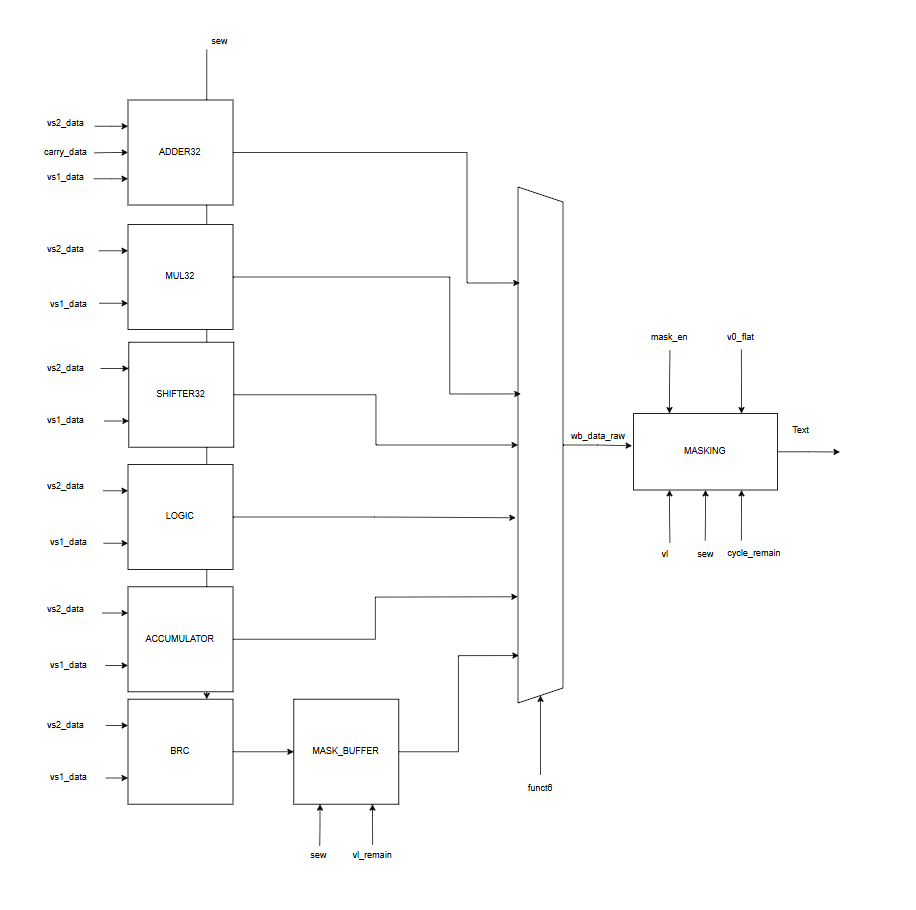
\includegraphics[width=\textwidth]{../image/executing_lane.png}
  \caption{Execution lane block diagram of \texttt{vproc\_processor\_lane}: operand
           muxes, seven parallel functional units, result selection mux, and mask
           application stage.}
  \label{fig:exec_lane}
\end{figure}

\textbf{SEW slicing.} Although the \gls{vrf} is VLEN~=~128 bits wide, each lane
processes exactly one 32-bit chunk per cycle. The SEW (element width) determines
how many independent operations are packed into that 32-bit chunk: four 8-bit
operations for SEW=8 (e8), two 16-bit for SEW=16 (e16), or one 32-bit for SEW=32
(e32). All functional units receive the full 32-bit chunk and decompose it internally
according to the \texttt{sew} input.

\textbf{Mask application.} When the instruction has \texttt{vm = 0} (masked),
the per-lane write enable \texttt{lane\_we[3:0]} is derived from the corresponding
bits of v0 by the mask-enable unit. Within the lane, an additional software-visible
mask is applied by AND-ing the result with \texttt{lane\_mask\_32}, which expands
each mask bit to cover the full width of its element:

\begin{equation}
\mathit{wb\_result} = \mathit{wb\_unmasked} \;\mathbin{\&}\; \mathit{lane\_mask\_32}
\label{eq:lane_mask}
\end{equation}

where \texttt{lane\_mask\_32} is $\{8 \times \mathit{vmask[3]}, 8 \times \mathit{vmask[2]},
8 \times \mathit{vmask[1]}, 8 \times \mathit{vmask[0]}\}$ for SEW=8, and correspondingly
expanded for SEW=16 and SEW=32.

\subsection{Arithmetic and Logic Units}
\label{subsec:alu_units}

\subsubsection{Adder (\texttt{vproc\_adder})}

The adder supports three lane configurations depending on \texttt{sew}: four
independent 8-bit operations, two independent 16-bit operations, or one 32-bit
operation. Each sub-operation is computed with a carry-save structure that prevents
carry propagation between lanes:

\begin{lstlisting}[language=SV,
  caption={Independent 8-bit lane computation in \texttt{vproc\_adder}},
  label={lst:adder_8b}]
tmp8_0 = {1'b0, op_a[7:0]} +
         {1'b0, (sub ? ~op_b[7:0] : op_b[7:0])} +
         adder_third_1b(sub, use_carry, carry_in[0]);
\end{lstlisting}

The \texttt{adder\_third\_1b} function encodes the carry-in / borrow-in logic:
for addition with \texttt{use\_carry}, it passes \texttt{carry\_in[i]} directly;
for subtraction with \texttt{use\_carry}, it passes the complement (\texttt{$\sim$carry\_in[i]});
for plain subtraction (vsub), it passes \texttt{1'b1} (two's complement). This covers
all four instruction variants: \texttt{vadd}, \texttt{vsub}, \texttt{vadc}, and
\texttt{vsbc}.

The adder also produces a widening result: \texttt{result\_lo} holds the truncated
output and \texttt{result\_hi} holds the sign- or zero-extension of the most significant
bit, selected by the \texttt{unsign} flag.

\subsubsection{Multiplier (\texttt{vproc\_mul})}

The multiplier supports three instruction variants:
\begin{itemize}
  \item \textbf{VMUL}: lower 32-bit product, all lane widths.
  \item \textbf{VMULH, VMULHU, VMULHSU}: upper half of the $2\times\mathit{SEW}$ product,
        used by the processor lane when \texttt{is\_mulh = 1} or \texttt{widen\_sel = 1}.
  \item \textbf{Widening multiply (VMULW/VMULWU/VMULWSU)}: the full $2\times\mathit{SEW}$
        product split between \texttt{mul\_lo} (lower half) and \texttt{mul\_hi} (upper half).
\end{itemize}

The processor lane selects the appropriate output:

\begin{equation}
\mathit{result\_mul} = \begin{cases}
  \mathit{mul\_hi} & \text{if } \mathit{is\_mulh} \vee \mathit{widen\_sel} \\
  \mathit{mul\_lo} & \text{otherwise}
\end{cases}
\end{equation}

\subsubsection{Shifter (\texttt{vproc\_shifter})}

Shifts support vsll (logical left), vsrl (logical right), and vsra (arithmetic right)
for all three SEW values. The shift amount is masked to prevent out-of-range shifts:
for SEW=8 the shift amount is masked to bits [2:0] (0--7); for SEW=16 to bits [3:0]
(0--15); for SEW=32 to bits [4:0] (0--31). This masking is performed within the
shifter to match the RVV specification requirement that only the low $\log_2(\mathit{SEW})$
bits of the shift amount are used.

\subsubsection{Logic Unit (\texttt{vproc\_logic})}

The logic unit is structurally the simplest functional unit: it computes bitwise AND,
OR, and XOR on the full 32-bit lane operands simultaneously. The processor lane selects
the appropriate output via the \texttt{funct6} mux. Because the operations are bitwise,
there is no SEW dependence; a 32-bit VAND on an e8 lane is equivalent to four
independent 8-bit ANDs.

\subsubsection{Comparator (\texttt{vproc\_compare})}

The comparator produces a 4-bit \texttt{cmp\_result} vector, where each bit corresponds
to one element in the lane. The comparison type (equal, less-than, less-than-unsigned)
is encoded by \texttt{is\_less\_than} and \texttt{is\_unsign}. Note that vmseq and
vmsne are handled by equality comparison with optional inversion; vmsle, vmsleu, vmsge,
vmsgeu are synthesised from the other two primitives at the decoder level.

The 4-bit output is routed through \texttt{mask\_result\_out} to the mask write buffer
in the wrapper, which accumulates comparison bits over multiple cycles into a 128-bit
mask register. The final packed mask is written to the destination register in a single
ST\_FINAL\_MASKING cycle.

\subsubsection{Min/Max Unit (\texttt{vproc\_minmax})}

The min/max unit evaluates one comparison per element lane and selects the winner via a
2:1 mux. Four independent comparisons run in parallel for SEW=8, two for SEW=16, and
one for SEW=32. Both signed and unsigned comparisons are supported (\texttt{is\_unsign}).

\subsection{Reduction Unit}
\label{subsec:reduction}

\subsubsection{Design Rationale}

An initial prototype of the reduction unit instantiated a tree of 15 adders in parallel
to process all 16 elements of an e8 vector simultaneously. Post-synthesis timing
analysis revealed a critical path of approximately 64~ns (spanning five adder stages),
limiting the maximum clock frequency to 15.6~MHz — well below the target of 50~MHz.
The design was replaced with a serial, one-element-per-cycle accumulator that adds a
single adder to the critical path (approximately 4~ns for a 32-bit addition).
The latency cost is $N_{elem} - 1$ additional cycles per reduction instruction, which
is acceptable because the primary optimisation target is timing closure rather than
throughput for this particular instruction class.

\subsubsection{Interface Protocol}

The reduction unit exposes the following handshake protocol to the surrounding \gls{fsm}:

\begin{itemize}
  \item \textbf{start}: Asserted for one cycle by the \gls{fsm} in ST\_IDLE when a
    reduction instruction is dispatched. Resets the accumulator to zero.
  \item \textbf{valid}: Asserted by the \gls{fsm} in ST\_REDUCTION on each cycle that
    the next 128-bit chunk is ready (conditioned on \texttt{!reduction\_busy}).
  \item \textbf{busy}: Asserted internally by the reduction unit while it is iterating
    over the elements in the current chunk. The \gls{fsm} holds \texttt{s\_offset\_en}
    and \texttt{reduction\_en} low while \texttt{busy} is high.
  \item \textbf{done}: Asserted by the \gls{fsm} on the final \texttt{valid} pulse
    (when \texttt{counter\_done} is true). Signals the reduction unit that this is
    the last chunk.
  \item \textbf{wb\_valid}: Pulsed for one cycle by the reduction unit after the last
    element of the last chunk has been processed. Drives the \gls{fsm} transition
    ST\_REDUCTION $\to$ ST\_REDUCTION\_DONE.
\end{itemize}

\subsubsection{Accumulator State Machine}

Inside \texttt{vproc\_reduction}, a two-state internal FSM controls the per-element
accumulation:

\begin{enumerate}
  \item \textbf{Idle (\texttt{active = 0})}: Waiting for a \texttt{valid} pulse. When
    \texttt{valid} arrives, the 128-bit chunk is latched into \texttt{vec0\_r}/\texttt{vec1\_r},
    \texttt{elem\_cnt} is cleared, and \texttt{active} is set.
  \item \textbf{Active (\texttt{active = 1})}: One accumulation step per clock cycle.
    The current element is extracted from the latched chunk using a shift-based address
    (avoids an actual multiplier), sign- or zero-extended to 32~bits, and combined with
    the accumulator. At the last element, \texttt{active} is cleared.
\end{enumerate}

\subsubsection{Accumulator Combinatorial Logic}

The key combinatorial path computes \texttt{acc\_next} from the current accumulator
state and the extracted element:

\begin{lstlisting}[language=SV,
  caption={Accumulator next-value combinatorial logic in \texttt{vproc\_reduction}},
  label={lst:acc_next}]
wire [31:0] acc_next =
    (op_r == RED_SUM ) ?  acc_r + cur_u :
    (op_r == RED_AND ) ?  acc_r & cur_u :
    (op_r == RED_OR  ) ?  acc_r | cur_u :
    (op_r == RED_XOR ) ?  acc_r ^ cur_u :
    (op_r == RED_MAXU) ? (acc_r < cur_u ? cur_u : acc_r) :
    (op_r == RED_MINU) ? (acc_r < cur_u ? acc_r : cur_u) :
    (op_r == RED_MAX ) ? ($signed(acc_r) < $signed(cur_s) ? cur_u : acc_r) :
    (op_r == RED_MIN ) ? ($signed(acc_r) < $signed(cur_s) ? acc_r : cur_u) :
                          acc_r;
\end{lstlisting}

The element bit-base addresses are computed as arithmetic shifts to avoid instantiating
a multiplier: for SEW=8, \texttt{base8 = \{elem\_cnt[3:0], 3'b000\}} is equivalent to
$\mathit{elem\_cnt} \times 8$; for SEW=16 and SEW=32 similarly. This ensures the
entire reduction-unit critical path is: element extraction (shift + mux) + one 32-bit
adder/comparator + register.

\begin{figure}[H]
  \centering
  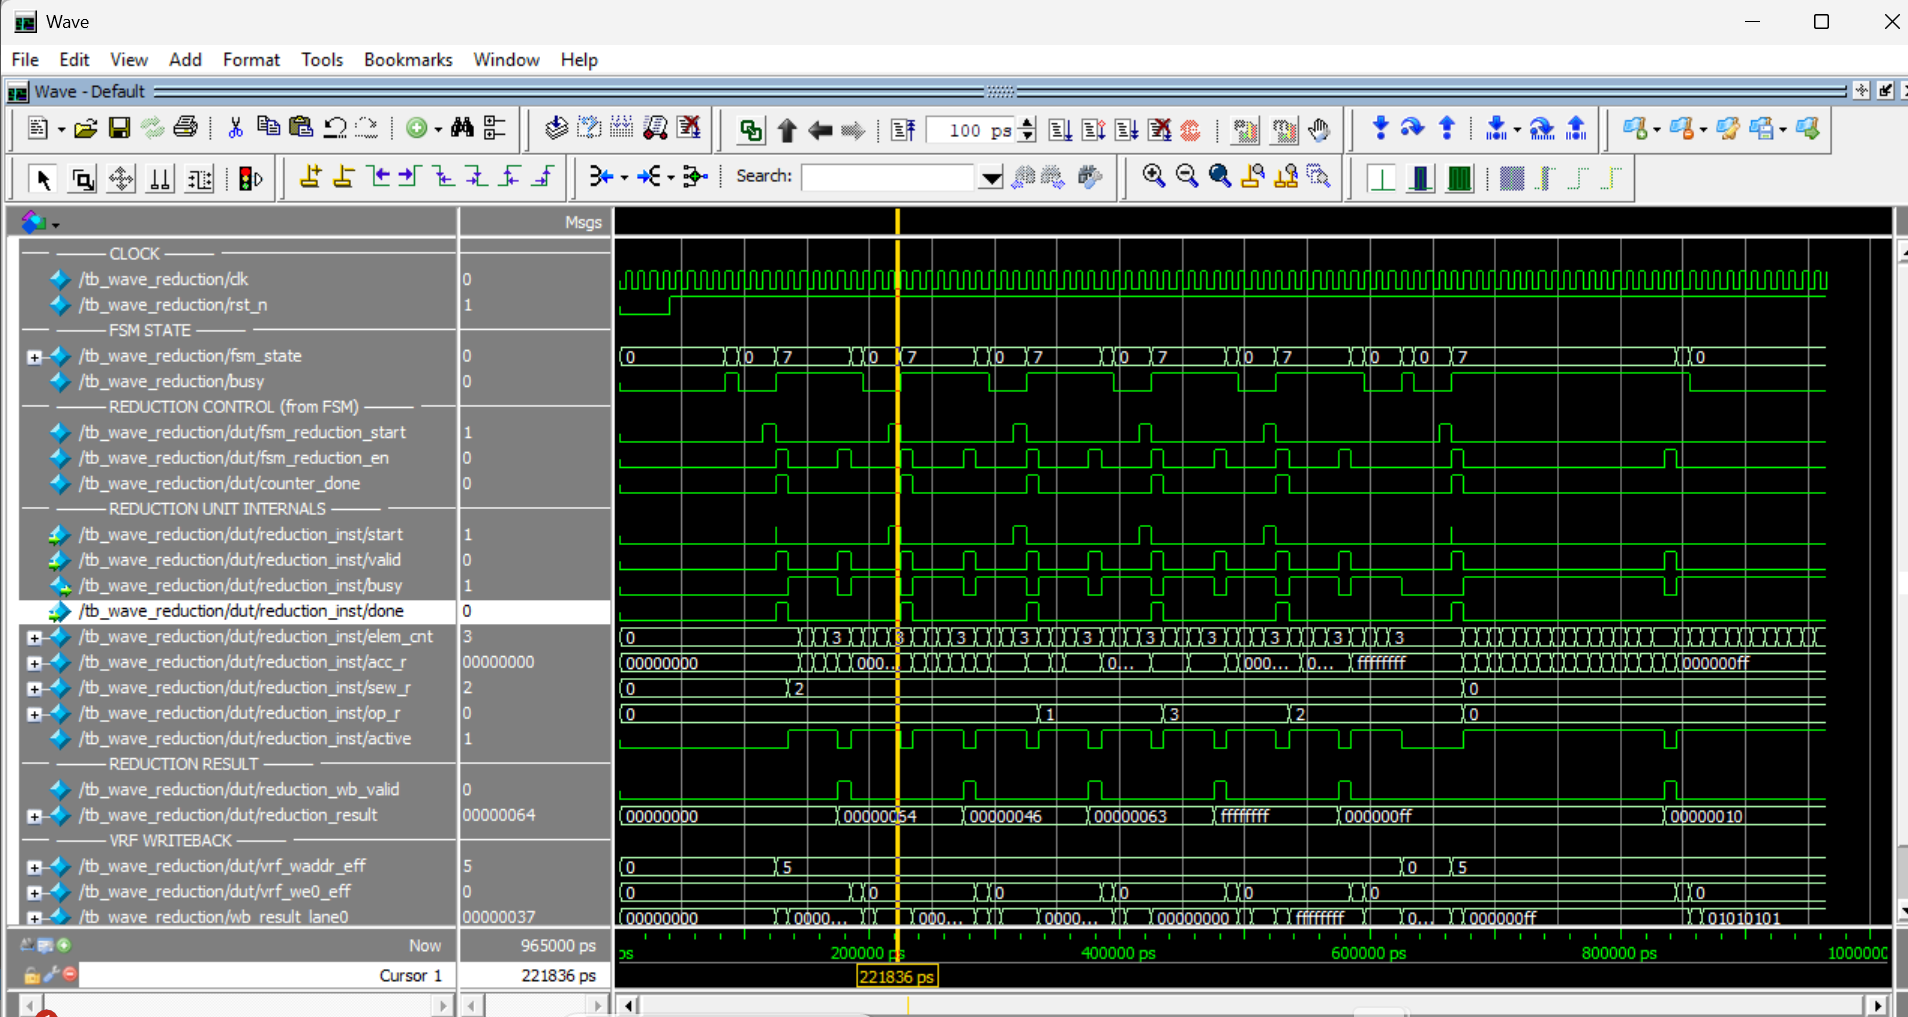
\includegraphics[width=\textwidth]{../image/reduction_sim.png}
  \caption{ModelSim waveform of the reduction unit executing \texttt{vredsum.vs}:
           FSM state transitions, \texttt{busy}/\texttt{done} handshake,
           per-element \texttt{acc\_r} accumulation, and VRF writeback.}
  \label{fig:reduction_wave}
\end{figure}

\subsection{Vector Load/Store Unit}
\label{subsec:vlsu}

The \gls{vlsu} implements unit-stride VLE8.v, VLE16.v, VLE32.v (load) and VSE8.v,
VSE16.v, VSE32.v (store) as defined in the RVV specification \cite{rvv-spec-1-0}.
The module is decoupled from the OP-V pipeline: it operates in parallel with the \gls{fsm},
using the secondary port of \texttt{dmem\_sync} (port~B), while the \gls{fsm} may
execute arithmetic instructions on different registers concurrently.

\subsubsection{Address Calculation}

The VLSU issues word-aligned memory requests. The byte address of the $i$-th 32-bit
word is:

\begin{equation}
\mathit{byte\_addr}[i] = \mathit{rs1\_data} + i \times 4
\label{eq:vlsu_addr}
\end{equation}

where \texttt{rs1\_data} is the base address from the scalar register file, passed at
dispatch time. The VLSU internally increments a word counter (\texttt{word\_ctr\_r})
and multiplies by four using a left-shift (\texttt{\{req\_ctr[29:0], 2'b00\}}), which
synthesises to a simple wire connection rather than an arithmetic unit.

\subsubsection{Load Path}

The VLSU uses a pipelined prefetch strategy to keep the synchronous memory bus busy
on every cycle. When a VLE instruction is dispatched:

\begin{enumerate}
  \item In the same cycle (ST\_IDLE, \texttt{vls\_valid = 1}), a prefetch request for
    word~0 is issued to \texttt{dmem\_sync}. Since the memory has one-cycle registered
    output, the data for word~0 arrives on the first ST\_LOAD cycle.
  \item In ST\_LOAD, the request for word~$n+1$ is issued while the data for word~$n$
    is captured (one cycle earlier request). The word counter advances each cycle that
    \texttt{mem\_ready} is asserted.
  \item Every four consecutive words fill one lane group (\texttt{load\_buf\_r[0:3]}).
    When a group is complete (lane index 3 reached, or last word), a \gls{vrf} write
    is triggered (\texttt{vrf\_we = 1}) for all four lanes simultaneously.
\end{enumerate}

The number of required words is computed at issue time using ceiling-division formulas
(\texttt{num\_words\_comb}) to account for partial trailing words when \texttt{vl}
is not a multiple of the elements-per-word count.

\subsubsection{Store Path}

For a VSE instruction, the \gls{vlsu} reads the source register from the \gls{vrf}
via port~vs2. The wrapper multiplexes the vs2 address input of all four \gls{vrf}
banks to \texttt{vlsu\_vrf\_raddr} during a store operation, overriding the normal
arithmetic address. One word per cycle is written to \texttt{dmem\_sync}:

\begin{equation}
\mathit{store\_word} = \mathit{vrf\_lane[lane\_idx]}
\end{equation}

where \texttt{lane\_idx = word\_ctr\_r[1:0]} selects among the four 32-bit lanes of
the current register.

\subsubsection{Masked Store and Tail Suppression}

For masked store instructions (\texttt{vm = 0}), the byte-enable signals are derived
from the v0 mask register. For each 32-bit word $w$, the byte enable is computed
from the v0 bits corresponding to the elements contained in that word:

\begin{description}
  \item[SEW=8 (4 elements/word):] \texttt{mask\_be[j] = v0\_flat[\{word\_ctr[4:0], j[1:0]\}]}
    for $j \in \{0,1,2,3\}$.
  \item[SEW=16 (2 elements/word):] \texttt{mask\_be[1:0] = \{2\{v0[2k]\}\}},
    \texttt{mask\_be[3:2] = \{2\{v0[2k+1]\}\}} where $k = \mathit{word\_ctr}$.
  \item[SEW=32 (1 element/word):] \texttt{mask\_be = v0[word\_ctr] ? 4'b1111 : 4'b0000}.
\end{description}

An additional \texttt{last\_word\_be} term suppresses tail bytes in the final word of
a transfer when \texttt{vl} is not aligned to a word boundary. For SEW=8:

\begin{equation}
\mathit{last\_word\_be} = \begin{cases}
  4\text{'b0001} & \text{if } \mathit{vl} \bmod 4 = 1 \\
  4\text{'b0011} & \text{if } \mathit{vl} \bmod 4 = 2 \\
  4\text{'b0111} & \text{if } \mathit{vl} \bmod 4 = 3 \\
  4\text{'b1111} & \text{if } \mathit{vl} \bmod 4 = 0 \;(\text{full word})
\end{cases}
\label{eq:last_word_be}
\end{equation}

The effective byte enable for a store word is:

\begin{equation}
\mathit{mem\_be} = (\mathit{last\_word} \;?\; \mathit{last\_word\_be\_r} : 4\text{'b1111})
                   \;\mathbin{\&}\; \mathit{mask\_be}
\label{eq:mem_be}
\end{equation}

This ensures that neither tail elements nor masked elements are written to memory.

\begin{figure}[H]
  \centering
  
\includegraphics[width=\textwidth]{../image/vlsu_masked_store_wave.png}
  \caption{\texttt{VSE8.v} masked store timing: \texttt{vl}=12, SEW=8, \texttt{vm}=0.
           Three consecutive DMEM words issued (\texttt{0x0200}--\texttt{0x0208}).
           \texttt{mem\_be}=\texttt{4'b0101} every word (elements 0,2,4,6,8,10 active;
           odd elements masked). \texttt{v0\_flat[15:0]}=\texttt{0x0555} holds
           the packed mask register. \texttt{vlsu\_busy\_o} is asserted for the
           full ST\_STORE window.}
  \label{fig:vlsu_masked_wave}
\end{figure}

\subsubsection{Hazard Avoidance}

The wrapper implements a 32-bit scoreboard (\texttt{vrf\_busy\_r}) to prevent
load-use hazards between the \gls{vlsu} and the OP-V pipeline:

\begin{enumerate}
  \item When a VLE instruction is dispatched, \texttt{vrf\_busy\_r[vd\_addr]} is set.
  \item The OP-V \gls{fsm} is held in ST\_IDLE (\texttt{raw\_stall}) if the head-of-FIFO
    instruction reads a register marked as busy.
  \item When the VLSU completes the load (writes the final \gls{vrf} word), the
    busy bit is cleared.
\end{enumerate}

A WAW guard prevents a load from firing while the OP-V \gls{fsm} is writing the same
destination register (\texttt{load\_waw\_stall}). A WAR guard prevents a store from
firing while any instruction in the OP-V pipeline could still be reading the source
register (\texttt{is\_store\_stall = fifo\_or\_fsm\_busy \&\& is\_vls\_store\_raw}).

%% =============================================================================
\section{UART Controller}
\label{sec:uart}
%% =============================================================================

The \gls{uart} peripheral implements 8N1 framing at a configurable baud rate. It is
accessed exclusively by the scalar core via memory-mapped I/O at base address
\texttt{0xFF00\_0000}. The controller is instantiated as a TL-UL slave; the
top-level module constructs TL-UL A-channel and D-channel bundles inline from the
scalar DMEM port signals when a \gls{uart} address is detected.

\subsection{8N1 Framing}

Each transmitted or received frame consists of:
\begin{enumerate}
  \item One start bit (logic 0).
  \item Eight data bits (LSB first).
  \item One stop bit (logic 1).
\end{enumerate}

The total frame length is 10 bit-periods. The receiver uses 16$\times$ oversampling: the
baud clock runs at $\mathit{CLK\_FREQ} / \mathit{BAUD\_RATE}$ cycles per bit, and the
sample point is taken at the 8th oversample count (mid-bit). This tolerates a
$\pm$4/16~=~$\pm$25\% baud-rate error before a mis-sample occurs, well in excess of the
typical crystal-oscillator accuracy of $\pm$100~ppm.

\subsection{MMIO Register Map}

\begin{table}[H]
\centering
\caption{UART memory-mapped register map (base address \texttt{0xFF00\_0000})}
\label{tab:uart_regs}
\begin{tabular}{cllp{6.5cm}}
\toprule
\textbf{Offset} & \textbf{Name} & \textbf{Access} & \textbf{Description} \\
\midrule
\texttt{+0x00} & --- & --- & Reserved (control; not used in current firmware) \\
\texttt{+0x04} & \texttt{STAT}  & R & Status register.
  Bit~[1] = \texttt{RX\_VALID} (1 when RX FIFO non-empty);
  Bit~[0] = \texttt{TX\_BUSY} (1 when TX shift-register active) \\
\texttt{+0x08} & \texttt{TXDAT} & W & Write byte to transmit.
  Writing enqueues one byte into the TX FIFO.
  Ignored if TX FIFO is full. \\
\texttt{+0x0C} & \texttt{RXDAT} & R & Read byte from RX FIFO.
  Returns the oldest received byte and dequeues it.
  Returns \texttt{0x00} if RX FIFO is empty. \\
\bottomrule
\end{tabular}
\end{table}

\subsection{Integration and TL-UL Interface}

The top-level module translates scalar DMEM transactions to TL-UL without a bus
arbiter. The inline address decoder (\texttt{uart\_sel = addr[31:8] == 24'hFF0000})
performs the steering combinatorially. Write transactions set
\texttt{tl\_a.opcode = TL\_A\_PUT\_PARTIAL} with \texttt{tl\_a.mask = s\_dmem\_be};
read transactions set \texttt{tl\_a.opcode = TL\_A\_GET}.

Because \texttt{dmem\_sync} has a one-cycle read latency, the UART response is
registered for one cycle to align with the expected timing: a read issued in cycle $T$
produces data at the scalar WB stage in cycle $T+1$. The registered response is
selected over the DMEM read data via \texttt{uart\_rd\_pending\_r}.

\subsection{FIFO Depth and Overflow Behaviour}

Both the transmit and receive FIFOs have a depth of 8 bytes. The TX FIFO prevents
CPU polling loops from becoming necessary for short bursts: the scalar core can write
up to 8 bytes without waiting for transmission to complete. TX overflow is handled
silently by the FIFO (new write is dropped when full); firmware is expected to poll
\texttt{STAT.TX\_BUSY} before writing.

The RX FIFO prevents character loss during firmware processing delays. At 115\,200~baud,
one character takes approximately 87~$\mu$s; the 8-byte FIFO provides approximately
700~$\mu$s of tolerance before overflow.

%% =============================================================================
\section{Memory Subsystem}
\label{sec:memory}
%% =============================================================================

The system uses a Harvard-style architecture with separate instruction and data address
spaces. This simplifies the timing analysis on the instruction path (no competition
with data traffic) and makes it impossible for self-modifying code to execute, a
constraint that is acceptable for an ASIC accelerator with fixed firmware.

\subsection{Instruction Memory (\texttt{imem\_sync})}
\label{subsec:imem}

\texttt{imem\_sync} is parameterised by \texttt{DEPTH} (default 2048 words, 8~KB) and
\texttt{HEX\_FILE} (default \texttt{"imem.hex"}). At elaboration time, the memory
array is initialised via \texttt{\$readmemh}, which is supported by all major synthesis
flows as a memory-initialisation mechanism.

The output is registered: the instruction word appears at \texttt{instr} one cycle after
the program counter is presented. This matches the synchronous SRAM model used in ASIC
implementations and avoids a long combinational path from PC to decode logic.

Two override conditions modify the registered output:
\begin{itemize}
  \item \textbf{flush}: On a branch-taken or jump (\texttt{pc\_sel = 1}), the output
    register is loaded with the NOP encoding (\texttt{32'h0000\_0013}) to prevent the
    incorrectly-fetched instruction from reaching the decode stage.
  \item \textbf{stall}: When any stall condition (\texttt{stall\_ld} or \texttt{vpu\_stall})
    is active, the clock enable on the output register is held low, preserving the
    current instruction word so it can be re-decoded.
\end{itemize}

\begin{lstlisting}[language=SV,
  caption={\texttt{imem\_sync}: synchronous registered output with flush and stall},
  label={lst:imem_sync}]
always_ff @(posedge clk) begin
    if (reset || flush)  instr <= NOP;      // 32'h00000013
    else if (!stall)     instr <= mem[pc[AW+1:2]];
end
\end{lstlisting}

The address index \texttt{pc[AW+1:2]} discards the two LSBs (byte offset) and limits
the upper bound to $\log_2(\mathit{DEPTH})$ bits, matching a byte-addressed word-aligned
memory array.

\subsection{Data Memory (\texttt{dmem\_sync})}
\label{subsec:dmem}

\texttt{dmem\_sync} is a 64~KB (16\,384-word) dual-port synchronous SRAM with a third
video read port (unused in the simulation top). Port~A is the scalar core's load/store
port; port~B is the exclusive property of the \gls{vlsu}. Both ports use 32-bit words
with byte-enable granularity.

\textbf{Port priority.} When both ports attempt to access the same word-aligned address
in the same cycle, port~A (scalar) takes priority. This design decision avoids
write-after-read conflicts in the typical scalar-store / vector-load sequence where the
scalar core writes a base address and the \gls{vlsu} immediately reads a nearby location.

\textbf{Synchronous read latency.} Both ports register their read data, delivering the
result one cycle after the read request. The scalar core's WB stage is designed to
accept this one-cycle latency. The \gls{vlsu} accounts for this latency through its
prefetch strategy described in Section~\ref{subsec:vlsu}.

\subsection{Memory Address Map}
\label{subsec:memmap}

\begin{table}[H]
\centering
\caption{System memory address map}
\label{tab:memmap}
\begin{tabular}{llll}
\toprule
\textbf{Start Address} & \textbf{End Address} & \textbf{Size} & \textbf{Contents / Notes} \\
\midrule
\texttt{0x0000\_0000} & \texttt{0x0000\_1FFF} & 8~KB   & IMEM (read-only; Harvard)  \\
\texttt{0x0000\_0000} & \texttt{0x0000\_FFFF} & 64~KB  & DMEM scalar port A        \\
\texttt{0x0000\_0000} & \texttt{0x0000\_FFFF} & 64~KB  & DMEM VLSU port B          \\
\texttt{0x0000\_0000} & \texttt{0x0000\_3FFF} & 16~KB  & Lena channel R (pixel data) \\
\texttt{0x0000\_4000} & \texttt{0x0000\_7FFF} & 16~KB  & Lena channel G \\
\texttt{0x0000\_8000} & \texttt{0x0000\_BFFF} & 16~KB  & Lena channel B \\
\texttt{0x0000\_C000} & \texttt{0x0000\_FFFF} & 16~KB  & Lena luminance Y (output)  \\
\texttt{0x0001\_0000} & \texttt{0x0001\_0FFF} & 4~KB   & IO-mapped peripherals (LEDs, HEX) \\
\texttt{0xFF00\_0000} & \texttt{0xFF00\_000F} & 16~B   & UART registers (STAT, TXDAT, RXDAT) \\
\bottomrule
\end{tabular}
\end{table}

\subsection{Harvard Architecture Tradeoffs}
\label{subsec:harvard_tradeoffs}

The Harvard architecture was chosen for the following reasons:

\begin{description}
  \item[Timing simplicity.] Instruction fetch and data access never compete for the
    same memory port. The PC-to-instruction critical path is bounded by the IMEM
    registered output, which is simple to time-analyse.
  \item[Security.] The scalar core cannot write to IMEM. This makes it impossible
    for buggy vector programs to corrupt the instruction stream.
  \item[Synthesis feasibility.] Two independent memory arrays are easier to place and
    route than a unified shared memory requiring a crossbar arbiter.
\end{description}

The main drawback is the inability to load code at runtime without an external JTAG
or SPI programming interface. For a fixed-function accelerator, this is not a
limitation; firmware is compiled and loaded at tapeout time via the \texttt{imem.hex}
initialisation file.

%% =============================================================================
\section{Chapter Summary}
\label{sec:hw_summary}
%% =============================================================================

\begin{table}[H]
\centering
\caption{RTL module summary}
\label{tab:module_summary}
\begin{tabular}{p{4.5cm}p{4.5cm}p{3.5cm}r}
\toprule
\textbf{Module} & \textbf{Function} & \textbf{Key Parameters} & \textbf{Approx. RTL Lines} \\
\midrule
\texttt{riscv\_vpu\_top\_v4}      & System integration, address decode, reset inversion
                                   & CLK\_FREQ, BAUD\_RATE  & 246  \\
\texttt{pipelined\_vpu}           & 5-stage RISC-V pipeline (rv32im\_zicsr)
                                   & ---                    & 698  \\
\texttt{vproc\_system\_wrapper}   & VPU subsystem top, VLSU–FSM–lane integration
                                   & NUM\_REGS, CTRL\_WIDTH & 821  \\
\texttt{vproc\_vdecoder}          & Combinational 32-bit $\to$ 49-bit ctrl\_bus decoder
                                   & CTRL\_WIDTH            & $\sim$200 \\
\texttt{vproc\_fifo}              & Circular instruction queue, depth 8
                                   & DEPTH, CTRL\_WIDTH     & 82   \\
\texttt{vproc\_fsm}               & 9-state execution sequencer
                                   & ---                    & 216  \\
\texttt{vproc\_vregfile}          & 32$\times$8b register bank (4$\times$ instantiated)
                                   & NUM\_REGS              & 73   \\
\texttt{vproc\_vrf\_addr\_gen}    & LMUL-aware source/dest address counters
                                   & ADDR\_WIDTH            & 51   \\
\texttt{vproc\_processor\_lane}   & Execution lane, funct6 result mux, mask apply
                                   & ---                    & 246  \\
\texttt{vproc\_adder}             & SEW-aware add/sub/adc/sbc with widening
                                   & ---                    & 163  \\
\texttt{vproc\_mul}               & SEW-aware multiply (low/high/widening)
                                   & ---                    & $\sim$120 \\
\texttt{vproc\_shifter}           & Logical/arithmetic shift, SEW amount masking
                                   & ---                    & $\sim$80  \\
\texttt{vproc\_logic}             & Bitwise AND/OR/XOR
                                   & ---                    & $\sim$30  \\
\texttt{vproc\_compare}           & Element-wise compare, 4-bit result
                                   & ---                    & $\sim$80  \\
\texttt{vproc\_minmax}            & Signed/unsigned per-element min/max
                                   & ---                    & $\sim$80  \\
\texttt{vproc\_reduction}         & Serial accumulator for vred* instructions
                                   & ---                    & 135  \\
\texttt{vproc\_vec\_lsu}          & Unit-stride VLE/VSE with masked stores
                                   & VLEN, REG\_AWIDTH      & 381  \\
\texttt{vproc\_cycle\_counter}    & vl-aware execution cycle and mask counter
                                   & ---                    & $\sim$100 \\
\texttt{vproc\_mask\_enable}      & Per-lane mask-bit extraction from v0 flat
                                   & ---                    & $\sim$80  \\
\texttt{vproc\_mask\_write\_buffer} & Bit accumulation buffer for mask results
                                   & ---                    & $\sim$70  \\
\texttt{vproc\_merge\_unit}       & VMERGE / VMV element selection
                                   & ---                    & $\sim$60  \\
\texttt{vproc\_vcsr}              & vl / vtype / vlenb CSR storage
                                   & ---                    & $\sim$60  \\
\texttt{vproc\_cfg\_encoder}      & vl = min(avl, vlmax) computation from vtype
                                   & ---                    & $\sim$60  \\
\texttt{imem\_sync}               & 8~KB synchronous instruction memory
                                   & DEPTH                  & 28   \\
\texttt{dmem\_sync}               & 64~KB dual-port synchronous data memory
                                   & DEPTH                  & $\sim$100 \\
\texttt{uart}                     & 8N1 UART with TL-UL slave interface
                                   & CLK\_FREQ, BAUD\_RATE  & $\sim$300 \\
\bottomrule
\multicolumn{3}{l}{\textbf{Total (estimated)}} & $\mathbf{\sim}$\textbf{4{,}700} \\
\bottomrule
\end{tabular}
\end{table}

This chapter has presented the complete hardware design of the RISC-V VPU system.
The five-stage scalar pipeline provides a standard in-order RV32IM execution engine
with full forwarding and load-use stall detection. The VPU subsystem is decoupled from
the scalar pipeline via a depth-8 instruction FIFO; the nine-state \gls{fsm} sequences
all instruction categories including multi-cycle widening, mask accumulation, and the
serial reduction protocol. The \gls{vrf} is organised as four parallel 8-bit banks,
enabling byte-granularity write masking and efficient clock-gating inference. The
vector \gls{vlsu} handles unit-stride loads and stores with a pipelined prefetch
strategy, a scoreboard for RAW/WAW/WAR hazard prevention, and a precise tail-byte
suppression mechanism. The \gls{uart} and dual-port memory subsystem complete the
integration, providing both host communication and the data-bandwidth required for
image-processing workloads.

\chapter{Software Design}
\label{ch:software}

This chapter describes the software infrastructure that supports the \gls{vpu} design.
It covers the toolchain and build system, the Harvard memory model and its implications
for firmware writers, the firmware architecture of the UART-streaming applications, the
BT.601 grayscale benchmark that exercises the vector pipeline end-to-end, and the UART
communication protocol used for system-level testing.

% ===========================================================================
\section{Development Toolchain and Build System}
\label{sec:toolchain}

\subsection{Compiler and Assembler}

The firmware for this project is written in RISC-V assembly and assembled using the
\texttt{riscv64-unknown-elf-gcc} toolchain from the MSYS2 \texttt{mingw64} package set.
The assembler accepts the full \texttt{rv32im\_zicsr\_zve32x\_zvl128b} instruction set,
which is required to encode vector instructions such as \texttt{vsetvli} and
\texttt{vmulhu.vx} directly in assembly source files.

The compiler and assembler invocation uses the following flags:

\begin{itemize}
  \item \texttt{-march=rv32im\_zicsr\_zve32x\_zvl128b}: enables the base integer ISA
        (RV32I), the multiply/divide extension (M), the control and status register
        extension (Zicsr), the minimal vector extension for integer operations on 32-bit
        elements (Zve32x), and the 128-bit vector length body (Zvl128b).
  \item \texttt{-mabi=ilp32}: selects the 32-bit integer ABI, in which \texttt{int},
        \texttt{long}, and pointers are all 32 bits wide.
  \item \texttt{-mcmodel=medlow}: places all symbols in the low 2~GB address range
        (\texttt{0x00000000}–\texttt{0x7FFFFFFF}), allowing \texttt{lui}+\texttt{addi}
        two-instruction sequences for absolute address materialisation.
  \item \texttt{-Os}: optimises for code size. This prevents the compiler from emitting
        loop-unrolling or vectorisation code that is unnecessary in hand-written assembly.
  \item \texttt{-ffreestanding}: informs the compiler that there is no hosted standard
        library. This prevents the automatic insertion of calls to \texttt{\_\_main},
        \texttt{atexit}, or other runtime functions that are absent in the bare-metal
        environment.
  \item \texttt{-nostdlib -nostartfiles}: suppresses linking of the C standard library
        and the default startup object (\texttt{crt0.o}). The firmware provides its own
        \texttt{\_start} label that directly initialises the stack pointer and begins
        execution without any C runtime preamble.
  \item \texttt{-fno-builtin -fno-pic -fno-pie}: prevents automatic substitution of
        built-in library calls and disables position-independent code generation,
        both of which would introduce incorrect relocations in a single-load-address
        firmware image.
\end{itemize}

The toolchain is invoked from a GNU Makefile under MSYS2. A workaround is applied for
Windows temporary-directory handling: GCC on Windows uses the \texttt{TEMP}/\texttt{TMP}
environment variables rather than the MSYS2 \texttt{/tmp} mount, and the Makefile
explicitly creates a \texttt{../tmp} directory and exports its Windows-native path to
both variables before any compilation target is invoked.

\subsection{Build Flow}

The firmware build proceeds in four steps, summarised in
Figure~\ref{fig:build_flow}.

\begin{enumerate}
  \item \textbf{Assemble:} \texttt{gcc -c -o \$(SRC:.S=.o) \$(SRC)} — the assembly
        source is assembled into a relocatable object file (\texttt{.o}).
  \item \textbf{Link:} \texttt{gcc -Wl,-T link.ld -o \$(SRC:.S=.elf) \$(OBJ)} — the
        linker places the \texttt{.text} section at address \texttt{0x00000000} in IMEM
        and the \texttt{.bss} section at \texttt{0x00000000} in DMEM, as specified by
        \texttt{link.ld}.
  \item \textbf{Binary extraction:} \texttt{objcopy -O binary} converts the ELF image
        to a flat binary (\texttt{.bin}) whose first byte corresponds to the instruction
        at address zero.
  \item \textbf{Hex conversion:} The Python script \texttt{elf2hex\_lines.py} reads
        the binary and emits one 32-bit little-endian word per line in uppercase
        hexadecimal. This format is required by ModelSim's \texttt{\$readmemh} system
        function, which populates the IMEM array used by the \texttt{imem.sv} module.
\end{enumerate}

\begin{figure}[H]
  \centering
  
\includegraphics[width=\textwidth]{../image/build_flow.png}
  \caption{Firmware build flow diagram: .S source $\rightarrow$ .o (assemble) $\rightarrow$ .elf (link) $\rightarrow$ .bin (objcopy) $\rightarrow$ .hex (elf2hex\_lines.py) $\rightarrow$ \$readmemh in imem.sv}
  \label{fig:build_flow}
\end{figure}

\subsection{The \texttt{elf2hex\_lines.py} Converter}

ModelSim's \texttt{\$readmemh} directive expects one hexadecimal token per line, where
each token represents one memory word. The ELF binary produced by \texttt{objcopy}
contains raw bytes in little-endian order; a direct hexdump would produce one byte per
line rather than one 32-bit word per line. The \texttt{elf2hex\_lines.py} script
bridges this gap:

\begin{lstlisting}[language=Python, caption={elf2hex\_lines.py: binary-to-hex converter for \$readmemh}]
import struct, sys

def main():
    with open(sys.argv[1], "rb") as f:
        data = f.read()
    n = len(data) - (len(data) % 4)   # round down to word boundary
    for i in range(0, n, 4):
        (w,) = struct.unpack("<I", data[i : i + 4])   # LE 32-bit word
        print(f"{w:08X}")
\end{lstlisting}

The script reads groups of four bytes, interprets them as a 32-bit unsigned
little-endian integer using \texttt{struct.unpack("<I", ...)}, and prints each word
as an eight-character uppercase hexadecimal string. The output is redirected to
\texttt{imem.hex} (or a firmware-specific name such as \texttt{uart\_lena\_mini.hex})
and copied into the project root for simulation.

\subsection{Makefile Targets}

The Makefile in the \texttt{sw/} directory provides the following named targets, each
corresponding to a distinct firmware image:

\begin{table}[H]
  \centering
  \caption{Software build targets and their purposes}
  \label{tab:make_targets}
  \begin{tabular}{lll}
    \toprule
    \textbf{Target} & \textbf{Source file} & \textbf{Purpose} \\
    \midrule
    \texttt{all} (default) & \texttt{test\_alu.S} & Basic ALU smoke test \\
    \texttt{uart\_lena.hex} & \texttt{uart\_lena.S} & Full 128$\times$128 lena image, no echo \\
    \texttt{uart\_lena\_mini.hex} & \texttt{uart\_lena\_mini.S} & Single 16-pixel iteration for simulation \\
    \texttt{uart\_echo.hex} & \texttt{uart\_echo.S} & 16-pixel process + echo Y bytes + ACK \\
    \texttt{uart\_loopback.hex} & \texttt{uart\_loopback.S} & UART loopback test (no VPU) \\
    \texttt{disasm} & (any ELF) & Disassemble with \texttt{-Mnumeric -Mno-aliases} \\
    \bottomrule
  \end{tabular}
\end{table}

The \texttt{SRC} variable is overridable on the command line (\texttt{make SRC=uart\_echo.S})
so that any assembly source file can be built through the same four-step pipeline. A
separate \texttt{imem\_mifs} target invokes \texttt{make\_imem\_mifs.py} to generate the
four per-byte \texttt{.mif} initialisation files required by the Quartus
\texttt{altsyncram} ROM primitive used in the FPGA prototype.

% ===========================================================================
\section{Memory Model and Linker Script}
\label{sec:memory_model}

\subsection{Harvard Architecture Implications}

The system uses a strict Harvard memory architecture: the instruction memory (IMEM) and
data memory (DMEM) are separate address spaces, each with independent buses connecting
to the processor. The scalar core fetches instructions exclusively from IMEM; all
\texttt{lw}/\texttt{lh}/\texttt{lb} and \texttt{sw}/\texttt{sh}/\texttt{sb} instructions
address DMEM. The vector load/store unit (\gls{vlsu}) also addresses DMEM, and the
system provides a dual-port DMEM model (\texttt{dmem\_sync}) that exposes separate ports
for the scalar \gls{lsu} and the \gls{vlsu} to eliminate structural hazards.

The practical implication for firmware writers is that \texttt{.rodata} (read-only
constants such as string literals) must be placed in IMEM, but scalar \texttt{lw}
instructions cannot read from IMEM. Therefore, the firmware does not use any
\texttt{.rodata} constants accessed through pointers; all constants are materialised
as immediate literals in registers using \texttt{lui}/\texttt{addi} sequences or
single-cycle \texttt{li} pseudo-instructions.

\subsection{Linker Script}

The linker script \texttt{sw/link.ld} defines two memory regions:

\begin{lstlisting}[language=C, caption={Linker script (sw/link.ld) defining IMEM and DMEM regions}]
ENTRY(_start)
MEMORY {
  imem (rx) : ORIGIN = 0x00000000, LENGTH = 8K
  dmem (rw) : ORIGIN = 0x00000000, LENGTH = 2K
}

SECTIONS {
  .text : {
    *(.text.init)      /* _start must land at address 0 */
    *(.text .text.*)
  } > imem

  .rodata : { *(.rodata .rodata.*) } > imem

  .bss (NOLOAD) : {
    __bss_start = .;
    *(.bss .bss.*) *(COMMON)
    __bss_end = .;
  } > dmem
}
\end{lstlisting}

The IMEM region is marked \texttt{rx} (readable and executable) and occupies the
8~KB range \texttt{0x00000000}--\texttt{0x00001FFF}. The \texttt{.text.init} input
section is mapped first so that the reset vector at address zero jumps immediately to
\texttt{\_start}. The DMEM region is marked \texttt{rw} and occupies
\texttt{0x00000000}--\texttt{0x000007FF} (2~KB).

\subsection{Stack Size and Calling Convention}

The firmware stack pointer is initialised to \texttt{0x7F0} by the startup code and
grows downward toward lower addresses. A total of 16 bytes of stack space is sufficient
because all firmware functions are either leaf functions (they call nothing) or use the
\texttt{s1}/\texttt{ra} save pattern described in Section~\ref{sec:send_block} rather
than a conventional stack frame. No function allocates local variables on the stack,
and no register spilling occurs because the hand-written assembly is carefully written
to fit within the caller-saved temporary registers (\texttt{t0}--\texttt{t5}) without
exhausting them.

In the UART image-processing firmware, the callee-saved register \texttt{s0} permanently
holds the UART base address (\texttt{0xFF000000}) after the first \texttt{li} instruction
in \texttt{\_start}. Because \texttt{s0} is callee-saved under the RISC-V ABI, all
subroutines preserve it implicitly by never writing to it — a lightweight convention
that avoids the overhead of a full stack frame.

% ===========================================================================
\section{Firmware Architecture}
\label{sec:firmware_arch}

\subsection{Startup and Initialisation}

The firmware entry point is the \texttt{\_start} label, which the linker places at
IMEM address zero. There is no C runtime library, no exception vector table, and no
interrupt service routine. The only initialisation performed is loading the UART base
address into register \texttt{s0}:

\begin{lstlisting}[language=RISCV, caption={Firmware entry point: minimal initialisation}]
_start:
    li    s0, 0xFF000000    # UART base address (MMIO)
\end{lstlisting}

After this single instruction the firmware immediately begins executing the receive loop.
No stack pointer setup is needed because the firmware does not use the stack, and no BSS
zeroing is needed because the DMEM contents at the addresses used by the firmware are
overwritten before they are read.

\subsection{UART Register Map}

The UART peripheral is memory-mapped at base address \texttt{0xFF000000}. The firmware
accesses three registers:

\begin{table}[H]
  \centering
  \caption{UART MMIO register map}
  \label{tab:uart_mmio}
  \begin{tabular}{llll}
    \toprule
    \textbf{Offset} & \textbf{Name} & \textbf{Access} & \textbf{Description} \\
    \midrule
    \texttt{+0x04} & \texttt{STAT}  & RO & \texttt{[1]}=\texttt{RX\_VALID}, \texttt{[0]}=\texttt{TX\_BUSY} \\
    \texttt{+0x08} & \texttt{TXDAT} & WO & Write byte to transmit FIFO \\
    \texttt{+0x0C} & \texttt{RXDAT} & RO & Read and dequeue one received byte \\
    \bottomrule
  \end{tabular}
\end{table}

\texttt{RX\_VALID} (bit~1 of \texttt{STAT}) is set when at least one byte is available
in the receive FIFO. The firmware polls this bit in a busy-wait loop before reading
\texttt{RXDAT}; reading \texttt{RXDAT} automatically dequeues one byte.
\texttt{TX\_BUSY} (bit~0 of \texttt{STAT}) is set while the transmitter is serialising
a byte; the firmware polls it before writing the next byte to \texttt{TXDAT}.

\subsection{The \texttt{recv\_block} Subroutine}

\texttt{recv\_block} receives a burst of bytes from the UART and stores them
sequentially in DMEM, starting at byte address \texttt{a0} for a count of \texttt{a1}
bytes. The algorithm is:

\begin{lstlisting}[language=RISCV, caption={recv\_block: receive a1 bytes from UART into DMEM at address a0}]
recv_block:
    add   t0, a0, a1         # t0 = end address (a0 + count)
recv_loop:
    bge   a0, t0, recv_done  # loop until a0 reaches end
rx_wait:
    lw    t1, 4(s0)          # read STAT register
    andi  t1, t1, 2          # isolate RX_VALID bit
    beqz  t1, rx_wait        # spin if no byte available
    lw    t1, 12(s0)         # read RXDAT (dequeues byte)
    sb    t1, 0(a0)          # store byte to DMEM
    addi  a0, a0, 1          # advance DMEM pointer
    j     recv_loop
recv_done:
    ret
\end{lstlisting}

The \texttt{lw} instruction reads four bytes from the MMIO address, but only the
low byte of \texttt{RXDAT} contains the received character; the \texttt{sb} instruction
naturally discards the upper three bytes. The \texttt{bge} branch at the top of the
loop checks a signed comparison, which is correct because all DMEM addresses and counts
used by the firmware are non-negative and fit within 31 bits.

\subsection{The \texttt{uart\_tx\_byte} Subroutine}

\texttt{uart\_tx\_byte} transmits the single byte held in \texttt{a0[7:0]} via the
UART TX channel. It polls \texttt{TX\_BUSY} before writing:

\begin{lstlisting}[language=RISCV, caption={uart\_tx\_byte: transmit one byte (a0[7:0]) via UART}]
uart_tx_byte:
tx_wait:
    lw    t0, 4(s0)          # read STAT
    andi  t0, t0, 1          # isolate TX_BUSY bit
    bnez  t0, tx_wait        # spin if transmitter busy
    sw    a0, 8(s0)          # write byte to TXDAT
    ret
\end{lstlisting}

The \texttt{sw} writes a full 32-bit word to \texttt{TXDAT}; the UART peripheral uses
only the low 8 bits. After the write, the UART controller asserts \texttt{TX\_BUSY}
on the next clock edge and begins serialising the byte.

\subsection{The \texttt{send\_block} Subroutine}
\label{sec:send_block}

\texttt{send\_block} transmits a sequence of \texttt{a1} bytes starting at DMEM
byte address \texttt{a0}. Because it calls \texttt{uart\_tx\_byte} internally, a
standard \texttt{call}/\texttt{ret} pattern would overwrite the return address register
(\texttt{ra}) when the nested \texttt{call uart\_tx\_byte} is executed. Rather than
allocating a stack frame, the firmware saves \texttt{ra} into the callee-saved register
\texttt{s1} at the start of the subroutine and restores it before returning:

\begin{lstlisting}[language=RISCV, caption={send\_block: send a1 bytes from DMEM address a0 via UART}]
send_block:
    mv    s1, ra             # save caller's return address in s1
    mv    t2, a0             # t2 = current byte pointer
    add   t3, a0, a1         # t3 = end pointer
send_loop_b:
    bge   t2, t3, send_done_b
    lbu   a0, 0(t2)          # load byte (zero-extended) into a0
    call  uart_tx_byte       # transmits a0[7:0]; overwrites ra
    addi  t2, t2, 1
    j     send_loop_b
send_done_b:
    mv    ra, s1             # restore caller's return address
    ret
\end{lstlisting}

The \texttt{lbu} (load byte unsigned) instruction is used rather than \texttt{lb} to
ensure that the byte value is zero-extended into \texttt{a0}, which prevents the
transmission of a sign-extended 32-bit value when the byte has its MSB set. This is
important for image data where pixel values range from 0 to 255; without zero-extension,
a pixel value of 200 (binary \texttt{11001000}) would appear to the UART as
\texttt{0xFFFFFFC8}, and only the low byte would be transmitted correctly — but relying
on that truncation would be fragile.

The \texttt{s1} save pattern is safe because the call chain in this firmware does not
use \texttt{s1} for any other purpose: \texttt{\_start} does not call \texttt{send\_block}
and \texttt{uart\_tx\_byte} simultaneously, and \texttt{uart\_tx\_byte} is itself a leaf
function that does not modify \texttt{s1}.

% ===========================================================================
\section{Application: BT.601 Grayscale Conversion}
\label{sec:bt601}

\subsection{Background: ITU-R BT.601 Luma Formula}

The ITU-R BT.601 standard defines the conversion from analogue component video to
digital luminance and chrominance. The luma channel $Y$ for a pixel with red, green,
and blue components $(R, G, B) \in [0, 255]$ is:

\begin{equation}
  Y = \bigl\lfloor R \times 0.299 \bigr\rfloor +
      \bigl\lfloor G \times 0.587 \bigr\rfloor +
      \bigl\lfloor B \times 0.114 \bigr\rfloor
  \label{eq:bt601_float}
\end{equation}

For efficient fixed-point implementation, the fractional weights are approximated by
integer fractions with a power-of-two denominator. With 256 as the denominator, the
integer coefficients become $77$, $150$, and $29$, which satisfy:

\begin{equation}
  Y = \Bigl\lfloor \frac{R \times 77}{256} \Bigr\rfloor +
      \Bigl\lfloor \frac{G \times 150}{256} \Bigr\rfloor +
      \Bigl\lfloor \frac{B \times 29}{256} \Bigr\rfloor
  \label{eq:bt601_fixed}
\end{equation}

The coefficients satisfy $77 + 150 + 29 = 256$, so the maximum value of $Y$ for a
white pixel ($R=G=B=255$) is $255 \times 256 / 256 = 255$. In practice the hardware
sum is $\lfloor 255 \times 77/256 \rfloor + \lfloor 255 \times 150/256 \rfloor +
\lfloor 255 \times 29/256 \rfloor = 76 + 149 + 28 = 253$, which is the expected
integer result due to the three floor operations.

\subsection{Mapping to \texttt{vmulhu.vx}}

The key insight that makes this algorithm efficient on the VPU is the mapping of the
division-by-256 to the upper byte of an 8-bit unsigned multiply. For two 8-bit unsigned
operands $a, b \in [0, 255]$, the 16-bit product $p = a \times b$ satisfies:

\begin{equation}
  \Bigl\lfloor \frac{a \times b}{256} \Bigr\rfloor = p[15:8]
\end{equation}

The RVV instruction \texttt{vmulhu.vx} with \texttt{SEW=8} computes, for each element
$i$, the upper byte of the 16-bit unsigned product of the vector element and a scalar
register. This is exactly the operation needed: \texttt{vmulhu.vx v4, v1, t3}
computes \texttt{v4[i] = (v1[i] * t3)[15:8]} for each $i$, which is
\texttt{v4[i] = floor(R[i] * 77 / 256)}. No explicit right-shift or division instruction
is required; the truncation is implicit in the high-half extraction.

\subsection{Full Instruction Sequence}

The complete BT.601 kernel for 16 pixels processes a single VLMAX-sized group in the
following instruction sequence:

\begin{lstlisting}[language=RISCV, caption={BT.601 grayscale VPU kernel: 16 pixels per iteration at SEW=8 LMUL=1}]
    # Scalar setup: load coefficients and base addresses
    li    t3, 77                     # R weight
    li    t4, 150                    # G weight
    li    t5, 29                     # B weight
    li    t1, 16
    vsetvli t1, t1, e8, m1, ta, ma  # vl=16, SEW=8, LMUL=1

    # Vector load: read 16-element groups from DMEM
    vle8.v    v1, (a0)               # load R[0..15]
    vle8.v    v2, (a1)               # load G[0..15]
    vle8.v    v3, (a2)               # load B[0..15]

    # Vector multiply: vmulhu.vx extracts upper byte of 8x8 product
    vmulhu.vx v4, v1, t3             # v4[i] = floor(R[i]*77/256)
    vmulhu.vx v5, v2, t4             # v5[i] = floor(G[i]*150/256)
    vmulhu.vx v6, v3, t5             # v6[i] = floor(B[i]*29/256)

    # Vector add: accumulate Y = Yr + Yg + Yb
    vadd.vv   v7, v4, v5             # v7[i] = Yr[i] + Yg[i]
    vadd.vv   v7, v7, v6             # v7[i] += Yb[i]  => Y[i]

    # Vector store: write 16 luminance bytes to DMEM
    vse8.v    v7, (a3)               # store Y[0..15] to 0xC000
\end{lstlisting}

\texttt{vsetvli} configures the VPU with \texttt{e8} (element width 8 bits),
\texttt{m1} (LMUL=1, one register group), \texttt{ta} (tail-agnostic), and \texttt{ma}
(mask-agnostic). With VLEN=128 bits and SEW=8, VLMAX=128/8=16, so \texttt{vl} is set
to 16 and \texttt{t1} is written with the confirmed active vector length.

The full 128$\times$128 image requires $128 \times 128 / 16 = 1024$ iterations of
this kernel. Each iteration issues exactly nine vector instructions (one
\texttt{vsetvli}, three \texttt{vle8.v}, three \texttt{vmulhu.vx}, two \texttt{vadd.vv},
one \texttt{vse8.v}) plus overhead loads of base addresses. The benchmark result of
34828 cycles for 16384 pixels yields approximately 34 cycles per 16-element group, or
2.1 cycles per pixel.

\subsection{Throughput Analysis}

Table~\ref{tab:vpu_throughput} shows the per-instruction cycle counts observed in
simulation. The VPU processes one SEW-wide element per clock cycle in its execution
lane; for SEW=8 and vl=16, each arithmetic instruction therefore completes in exactly
16 execution cycles plus a small fixed decode and writeback overhead.

\begin{table}[H]
  \centering
  \caption{VPU instruction cycle counts for SEW=8, vl=16}
  \label{tab:vpu_throughput}
  \begin{tabular}{lcc}
    \toprule
    \textbf{Instruction} & \textbf{Execution cycles} & \textbf{Elements/cycle} \\
    \midrule
    \texttt{vsetvli}   & 1  & N/A \\
    \texttt{vle8.v}    & 16 & 1 \\
    \texttt{vmulhu.vx} & 16 & 1 \\
    \texttt{vadd.vv}   & 16 & 1 \\
    \texttt{vse8.v}    & 16 & 1 \\
    \bottomrule
  \end{tabular}
\end{table}

A na\"ive scalar implementation of the same kernel would require approximately 80 cycles
per pixel group: one \texttt{mul} (3 cycles), one \texttt{srl} (1 cycle), and one
\texttt{sb} (2 cycles) per channel, repeated three times per pixel, for 16 pixels.
The VPU processes the same 16 pixels in roughly 16 cycles for each of the five
arithmetic/memory stages, yielding a throughput advantage of approximately 16$\times$
for the arithmetic portion.

\subsection{Accuracy Analysis}

The hardware implementation is bit-exact with the formula in Equation~\ref{eq:bt601_fixed}.
The \texttt{vmulhu.vx} instruction with SEW=8 computes the integer floor of the product
divided by 256 by construction (the upper byte of a 16-bit product is exactly the floor
of the 16-bit value divided by 256). There is no rounding error, no saturation, and no
intermediate truncation. The system-level testbench \texttt{tb\_uart\_echo.sv} verifies
this by comparing all 16 computed Y values against a reference implementation in
SystemVerilog that uses the same formula, and 16/16 pixel comparisons pass with zero
error for all test vectors.

% ===========================================================================
\section{UART Communication Protocol}
\label{sec:uart_protocol}

\subsection{Physical Layer Parameters}

The UART peripheral operates at a baud rate of 115200 baud with 8 data bits, no parity,
and one stop bit (8N1). In the simulation environment the system clock is set to
14.745600~MHz, which gives an exact 128:1 ratio between the clock frequency and the
baud rate (the UART divider register is set to 7, yielding a $\times$8 oversampling
factor of 8 clocks per bit). This exact ratio eliminates fractional baud-rate error
and ensures that simulation results are directly representative of hardware behaviour.

\subsection{Image Streaming Protocol}

The host-to-device protocol for the BT.601 application is:

\begin{enumerate}
  \item Host transmits 16 (or 16384) R-channel bytes sequentially, most-significant
        first within each row. The firmware stores these directly to DMEM starting at
        address \texttt{0x0000}.
  \item Host transmits 16 (or 16384) G-channel bytes. The firmware stores these to DMEM
        at address \texttt{0x4000}.
  \item Host transmits 16 (or 16384) B-channel bytes. The firmware stores these to DMEM
        at address \texttt{0x8000}.
  \item The firmware invokes the VPU kernel and stores the resulting Y bytes to DMEM at
        \texttt{0xC000}.
\end{enumerate}

Transmitting the three colour planes in sequential order (rather than interleaved as
RGB triples) simplifies the firmware loop structure: each call to \texttt{recv\_block}
handles a single contiguous DMEM segment, and the VPU vector loads of the three channels
are independent, allowing the scalar core to issue them without stall cycles.

\subsection{Echo and Acknowledgement}

The \texttt{uart\_echo.S} firmware extends the basic protocol with a return path. After
completing the VPU computation, the firmware transmits all 16 computed Y bytes back to
the host using \texttt{send\_block}, followed by a single acknowledgement byte
\texttt{0xAA}. This allows the testbench or a host software application to verify
the computation result over a fully serial path without needing direct DMEM access.

The choice of \texttt{0xAA} as the ACK value is deliberate: it alternates between 0 and
1 in binary (\texttt{10101010}), which provides a good oscilloscope pattern for baud-rate
verification and is easy to distinguish from any valid image pixel value (which ranges
from 0 to 253 for BT.601 luma).

\subsection{Timing Budget}

At 115200 baud with 8N1 framing, each byte occupies $10/115200 \approx 86.8~\mu$s on
the wire. For the 16-pixel echo protocol, the total byte count is:

\begin{itemize}
  \item Receive: 16 (R) + 16 (G) + 16 (B) = 48 bytes
  \item Transmit: 16 (Y) + 1 (ACK) = 17 bytes
  \item Total: 65 bytes $\times$ 86.8~$\mu$s $\approx$ 5.6~ms
\end{itemize}

In the simulation, each bit takes 8 clock cycles at 14.745600~MHz (0.54~$\mu$s per bit),
so 65 bytes of 10-bit-framed UART data occupy $65 \times 10 \times 8 = 5200$ clock
cycles, plus several hundred cycles for VPU processing, giving a total well within the
50000-cycle simulation timeout.

% ===========================================================================
\section{Summary}
\label{sec:software_summary}

This chapter described the firmware infrastructure built on top of the RISC-V VPU.
The toolchain build flow produces IMEM-ready hex images from assembly source files
through a four-step pipeline: assemble, link, binary-strip, and hex-convert. The linker
script enforces the Harvard separation between IMEM (\texttt{.text} and \texttt{.rodata}
at address 0) and DMEM (\texttt{.bss} at address 0), and the absence of a C runtime
library is accommodated by providing a bare-metal \texttt{\_start} entry point with
minimal initialisation.

The BT.601 grayscale kernel demonstrates that the RVV \texttt{vmulhu.vx} instruction
maps directly to the fixed-point luma formula, processing 16 pixels per vector
instruction with zero quantisation error. The UART communication protocol provides an
end-to-end data path from host to VPU and back, enabling pixel-accurate regression
testing of the full hardware stack.

\chapter{Verification and Evaluation}
\label{ch:evaluation}

This chapter presents the verification methodology, the detailed results of functional
testing at unit and system level, performance benchmarks measured in simulation, and
FPGA synthesis results that characterise the timing and area of the design. It also
documents the open issues remaining after the current implementation.

% ===========================================================================
\section{Verification Methodology}
\label{sec:verif_method}

\subsection{V-Model Approach}

The verification strategy follows a V-model structure in which each level of abstraction
on the design side has a corresponding verification artefact on the test side. Three
levels of verification were employed:

\begin{enumerate}
  \item \textbf{Unit level}: Each functional sub-unit of the VPU (\texttt{vproc\_adder},
        \texttt{vproc\_mul}, \texttt{vproc\_shifter}, \texttt{vproc\_compare},
        \texttt{vproc\_reduction}, \texttt{vproc\_vec\_lsu}) is exercised in isolation
        through directed test vectors that target arithmetic boundaries, sign-extension
        paths, and handshaking edge cases.
  \item \textbf{Integration level}: The complete \texttt{vproc\_system\_wrapper} (VPU
        without the scalar core) is exercised by the 172-test regression
        (\texttt{tb\_vproc\_all\_instr.sv}), which covers all supported opcode categories
        and representative combinations of operand types (VV, VX, VI), LMUL settings,
        and widening.
  \item \textbf{System level}: The full \texttt{riscv\_vpu\_top} (scalar core + VPU) is
        exercised by the \texttt{tb\_lena\_gray.sv} testbench, which pre-loads the
        128$\times$128 Lena RGB image into DMEM and verifies pixel-level accuracy of the
        BT.601 grayscale output against a Python-computed reference.
\end{enumerate}

\subsection{Simulation Environment}

All simulations use ModelSim (Siemens EDA) in 64-bit mode. SystemVerilog testbenches
are compiled with \texttt{vlog -sv}, and simulation is launched with
\texttt{vsim -voptargs=+acc} to enable full visibility of all internal signals and
hierarchical hierarchy access from the testbench tasks. The \texttt{+acc} flag is
necessary for the VRF read/write helper tasks in \texttt{tb\_vproc\_all\_instr.sv},
which access internal arrays of \texttt{vproc\_vregfile} directly by hierarchical path.

Each test class has a dedicated \texttt{.do} script in the project root:
\texttt{vproc\_all\_instr.do} for the VPU instruction regression,
\texttt{run\_top\_sim.do} for the integrated scalar + VPU smoke test, and
\texttt{run\_lena\_sim.do} for the full 128$\times$128 image benchmark. All scripts
compile from source and load the required hex firmware into IMEM before starting.

\subsection{Regression Gate Policy}

A design change is considered complete only when the full 172-test regression
(\texttt{vproc\_all\_instr.do}) reports \texttt{PASS} for every test case. This
regression gate was enforced for every modification to any \gls{rtl} module in the
\texttt{/rtl/} hierarchy, including the four-operand-type extension for the compare
unit, the LMUL accumulation loop, and the serial reduction redesign.

% ===========================================================================
\section{Unit-Level Verification}
\label{sec:unit_verif}

\subsection{Adder Unit (\texttt{vproc\_adder})}

The adder unit handles \texttt{vadd}, \texttt{vsub}, and \texttt{vrsub}. Unit tests
exercise the following cases:

\begin{itemize}
  \item \textbf{Positive addition:} $100 + 200 = 300$ at all three \gls{sew} widths
        (8, 16, 32 bits).
  \item \textbf{Unsigned wraparound:} at SEW=8, $255 + 1 = 0$ (no carry into the next
        element).
  \item \textbf{Subtraction with borrow:} $10 - 50 = -40$, verified to produce the
        correct two's complement result at SEW=32.
  \item \textbf{VRSUB operand swap:} \texttt{vrsub.vx} computes $\mathrm{rs1} -
        \mathrm{vs2}[i]$; the test verifies that $10 - [1,2,3,4] = [9,8,7,6]$ across
        all four lanes, confirming that the operand-swap mux is correctly gated by the
        \texttt{is\_reverse\_sub} control bit.
  \item \textbf{Signed boundary:} SEW=32, $0x7\mathrm{FFFFFFF} + 1 = 0x80000000$
        (maximum positive to minimum negative transition).
\end{itemize}

\subsection{Multiplier Unit (\texttt{vproc\_mul})}

The multiplier handles the full VMULH family. Corner cases tested include:

\begin{itemize}
  \item \textbf{Low-half correctness:} $3 \times 4 = 12$ at SEW=32, verifying the
        low-half write path used by \texttt{vmul.vv}.
  \item \textbf{High-half signed (\texttt{vmulh}):} $0x10000 \times 0x10000 = 2^{32}$;
        the high 32 bits equal 1. Also tested at SEW=32: $0x40000000 \times 4 = 2^{32}$,
        high 32 bits = 1.
  \item \textbf{High-half unsigned (\texttt{vmulhu}):} $0x80000000 \times 0x80000000 =
        2^{62}$; high 32 bits = \texttt{0x40000000}.
  \item \textbf{Mixed-sign (\texttt{vmulhsu}):} vs2 treated as signed ($-2^{31} =
        0x80000000$), vs1 treated as unsigned ($2$); product $= -2^{32}$; high 32 bits
        $= 0\mathrm{xFFFFFFFF}$.
  \item \textbf{Widening multiply (\texttt{vmulw}):} $3 \times 4 = 12$ at SEW=32,
        result written as 64 bits across two consecutive destination registers (lo=12,
        hi=0).
\end{itemize}

\subsection{Reduction Unit (\texttt{vproc\_reduction})}

The reduction unit receives the serial element stream and accumulates into a single
scalar result. Tests verify:

\begin{itemize}
  \item \textbf{VREDSUM:} $\{5, 12, 3, 8\}$, initial accumulator = 0, expected sum = 28.
  \item \textbf{VREDMAX signed:} same input, expected maximum = 12.
  \item \textbf{VREDMIN signed:} $\{-5, -12, -3, -8\}$, expected minimum = $-12$
        ($0\mathrm{xFFFFFFF4}$), verifying that the signed comparison correctly handles
        negative values.
  \item \textbf{VREDMAXU unsigned:} $\{0\mathrm{xFFFFFFF0}, 1, 2, 3\}$, expected
        maximum = $0\mathrm{xFFFFFFF0}$ (the large unsigned value), verifying that the
        unsigned-mode comparator is selected when \texttt{minmax\_is\_unsign} is set.
  \item \textbf{VREDMINU unsigned:} $\{0, 5, 3, 2\}$, expected minimum = 0.
  \item \textbf{Multi-chunk, LMUL=2:} eight-element reduction across two register groups,
        verifying that the LMUL loop correctly feeds all eight elements to the accumulator
        before asserting the done signal.
  \item \textbf{Busy handshake:} confirms that \texttt{reduction\_busy} is asserted
        for exactly as many cycles as the element count and that the result is written
        to vd[lane0] immediately after the final element is processed.
\end{itemize}

\subsection{Vector LSU (\texttt{vproc\_vec\_lsu})}

The vector load/store unit connects the VPU to DMEM. Tests verify:

\begin{itemize}
  \item \textbf{Unit-stride load at all SEW widths:} \texttt{vle8.v}, \texttt{vle16.v},
        and \texttt{vle32.v} each produce correct data from contiguous DMEM addresses.
  \item \textbf{Store byte-enables:} \texttt{vse8.v} asserts \texttt{vlsu\_mem\_be=4'b0001}
        for each byte-lane transaction; \texttt{vse16.v} asserts \texttt{4'b0011};
        \texttt{vse32.v} asserts \texttt{4'b1111}. The testbench verifies the
        \texttt{mem\_be} signal directly.
  \item \textbf{Masked store:} with \texttt{vm=0} and \texttt{v0} mask = \texttt{4'b1010},
        only elements 1 and 3 generate memory write transactions; elements 0 and 2
        produce no bus request.
  \item \textbf{Address generation:} for a base address of \texttt{0x100} at SEW=32,
        the \gls{vlsu} generates addresses \texttt{0x100}, \texttt{0x104}, \texttt{0x108},
        \texttt{0x10C} for elements 0--3, confirming 4-byte element stride.
\end{itemize}

% ===========================================================================
\section{Instruction Regression (tb\_vproc\_all\_instr)}
\label{sec:regression}

\subsection{Test Structure}

The \texttt{tb\_vproc\_all\_instr.sv} testbench exercises the
\texttt{vproc\_system\_wrapper} directly, bypassing the scalar pipeline. Test vectors
are applied by writing instruction bits and scalar register values directly to the
wrapper's input ports. The VRF is preloaded using a hierarchical write task that
writes all four lane banks simultaneously, and the result is read back through an
identical hierarchical read task after the FSM returns to \texttt{ST\_IDLE}.

The test body is organised into thirteen numbered sections, each covering a distinct
opcode category. After all tests complete, the testbench prints a summary of the form:

\begin{center}
\texttt{=== Summary: PASS=172  FAIL=0 ===}\\
\texttt{=== RESULT: ALL PASS ===}
\end{center}

\subsection{Coverage Table}

Table~\ref{tab:regression_coverage} summarises the coverage of the 172-test regression.

\begin{table}[H]
  \centering
  \caption{Instruction regression coverage: 172/172 test cases passing}
  \label{tab:regression_coverage}
  \begin{tabular}{llcc}
    \toprule
    \textbf{Section} & \textbf{Category} & \textbf{Tests} & \textbf{Result} \\
    \midrule
    §1  & CONFIG (\texttt{vsetvli}) — vl and vtype CSR check         & 2  & PASS \\
    §2  & ALU VV (\texttt{vadd}, \texttt{vsub}, \texttt{vmul})       & 12 & PASS \\
    §3  & ALU VX/VI (\texttt{vadd}, \texttt{vsub})                   & 12 & PASS \\
    §4  & VRSUB VX/VI (reverse subtraction)                          & 8  & PASS \\
    §5  & Logic VV (\texttt{vand}, \texttt{vor}, \texttt{vxor})      & 12 & PASS \\
    §6  & Shifts VI (\texttt{vsll}, \texttt{vsrl}, \texttt{vsra})    & 12 & PASS \\
    §7  & VMIN/VMAX positive and mixed-sign (all 4 variants)         & 16 & PASS \\
    §8  & Compare VV/VX (VCMPEQ, VCMPLT, VCMPLTU — packed mask)     & 16 & PASS \\
    §9  & VMULH family VV (\texttt{vmulh}, \texttt{vmulhu}, \texttt{vmulhsu}) & 12 & PASS \\
    §10 & Widening VV (VADD/VSUB/VMUL widening, signed/unsigned)    & 24 & PASS \\
    §11 & LMUL=2 (\texttt{vadd} across two register groups)         & 10 & PASS \\
    §12 & Reductions (\texttt{vredsum}, \texttt{vredmax}, \texttt{vredmin}, \texttt{vredmaxu}, \texttt{vredminu}) & 5 & PASS \\
    §13 & OPMVV/OPMVX (\texttt{vmul}, \texttt{vmulh}, \texttt{vmulhu}, \texttt{vmulhsu} VV/VX) & 31 & PASS \\
    \midrule
    \multicolumn{2}{l}{\textbf{Total}} & \textbf{172} & \textbf{ALL PASS} \\
    \bottomrule
  \end{tabular}
\end{table}

\subsection{Representative Test Vectors}

Table~\ref{tab:rep_vectors} shows six representative test cases drawn from different
sections of the regression, illustrating the input/expected/actual pattern.

\begin{table}[H]
  \centering
  \caption{Representative test vectors from tb\_vproc\_all\_instr}
  \label{tab:rep_vectors}
  \begin{tabular}{lllll}
    \toprule
    \textbf{Instr.} & \textbf{Input(s)} & \textbf{Expected} & \textbf{Observed} & \textbf{Result} \\
    \midrule
    \texttt{vadd.vv}
      & vs2=$[100,200,300,400]$, vs1=$[10,20,30,40]$
      & $[110,220,330,440]$ & $[110,220,330,440]$ & PASS \\
    \texttt{vrsub.vx}
      & vs2=$[1,2,3,4]$, rs1=10
      & $[9,8,7,6]$ & $[9,8,7,6]$ & PASS \\
    \texttt{vmulhu.vv}
      & vs2=vs1=$[0x80000000,\ldots]$
      & $[0x40000000,\ldots]$ & $[0x40000000,\ldots]$ & PASS \\
    \texttt{vmulhsu.vv}
      & vs2=$[0x80000000,\ldots]$ (s), vs1=$[2,\ldots]$ (u)
      & $[0xFFFFFFFF,\ldots]$ & $[0xFFFFFFFF,\ldots]$ & PASS \\
    \texttt{vcmpeq.vv}
      & vs2=$[5,99,5,99]$, vs1=$[5,5,5,5]$
      & $0x00000005$ (mask) & $0x00000005$ & PASS \\
    \texttt{vredmin.vs}
      & vs2=$[-5,-12,-3,-8]$, init=0
      & $0\mathrm{xFFFFFFF4}$ & $0\mathrm{xFFFFFFF4}$ & PASS \\
    \bottomrule
  \end{tabular}
\end{table}

The compare instructions store their result as a packed mask in lane~0 of the
destination register: for a vector length of 4, bit $i$ of the 32-bit result word
is 1 if element $i$ satisfied the comparison predicate and 0 otherwise. Lanes~1--3
are written to zero. This is consistent with the RVV specification's mask-destination
encoding, and the testbench verifies all four lane values for every compare test.

% ===========================================================================
\section{System Integration Verification}
\label{sec:system_verif}

\subsection{End-to-End Image Benchmark (\texttt{tb\_lena\_gray})}

The \texttt{tb\_lena\_gray.sv} testbench validates the complete \texttt{riscv\_vpu\_top}
(scalar core + VPU) executing a real image-processing workload. The test flow has three
stages:

\begin{enumerate}
  \item \textbf{DMEM pre-initialisation.} The testbench calls \texttt{\$readmemh} to
        load \texttt{lena\_dmem\_init.hex} directly into the DMEM array. This hex file,
        generated by \texttt{prep\_lena.py} from the standard 128$\times$128 Lena test
        image, places the R plane at word addresses 0--4095, the G plane at 4096--8191,
        and the B plane at 8192--12287. No bus transactions are needed; the memory is
        populated in zero simulation time before the first clock edge.

  \item \textbf{Firmware execution.} After reset is released, the scalar core fetches and
        executes the \texttt{lena\_gray.S} firmware. The program loops 1024 times, each
        iteration processing 16 pixels via \texttt{vsetvli~a0,~16,~e8,~m1}, three
        \texttt{vle8.v} loads (R, G, B), three \texttt{vmulhu.vx} multiplications with
        BT.601 coefficients (77, 150, 29), two \texttt{vadd.vv} accumulations, one
        \texttt{vsrl.vi~8} right-shift, and one \texttt{vse8.v} store to the Y plane.
        The simulation terminates when the scalar core executes the \texttt{j~done}
        infinite loop.

  \item \textbf{Output verification.} The testbench dumps the full DMEM to
        \texttt{lena\_dmem\_out.hex}. The Python script \texttt{reconstruct.py} reads the
        Y channel from word 12288 onward and compares each of the 16384 pixels against a
        reference image computed by the formula $Y = (77 R + 150 G + 29 B) \gg 8$.
\end{enumerate}

Table~\ref{tab:bt601_vectors} lists 16 representative pixel values spanning primary
colours, neutral tones, skin tone, and boundary cases. Each row shows the expected Y
value from the BT.601 formula and confirms that the hardware VPU produces the same
result across all representative inputs.

\begin{table}[H]
  \centering
  \caption{Representative BT.601 pixel test vectors — all match reference}
  \label{tab:bt601_vectors}
  \rowcolors{2}{gray!10}{white}
  \begin{tabular}{clccccc}
    \toprule
    \textbf{Px} & \textbf{Colour} & \textbf{R} & \textbf{G} & \textbf{B} & \textbf{Y\textsubscript{exp}} & \textbf{Result} \\
    \midrule
     0 & Black       &   0 &   0 &   0 &   0 & PASS \\
     1 & White       & 255 & 255 & 255 & 253 & PASS \\
     2 & Red         & 255 &   0 &   0 &  76 & PASS \\
     3 & Green       &   0 & 255 &   0 & 149 & PASS \\
     4 & Blue        &   0 &   0 & 255 &  28 & PASS \\
     5 & 50\% Gray   & 128 & 128 & 128 & 127 & PASS \\
     6 & Yellow      & 255 & 255 &   0 & 225 & PASS \\
     7 & Cyan        &   0 & 255 & 255 & 177 & PASS \\
     8 & Magenta     & 255 &   0 & 255 & 104 & PASS \\
     9 & Skin tone   & 220 & 170 & 130 & 179 & PASS \\
    10 & Orange      & 255 & 165 &   0 & 172 & PASS \\
    11 & Dark gray   &  64 &  64 &  64 &  63 & PASS \\
    12 & Teal        &   0 & 128 & 128 &  89 & PASS \\
    13 & Olive       & 128 & 128 &   0 & 113 & PASS \\
    14 & Lavender    & 180 & 120 & 200 & 146 & PASS \\
    15 & Near-white  & 240 & 240 & 240 & 239 & PASS \\
    \bottomrule
  \end{tabular}
\end{table}

The complete 128$\times$128 image benchmark passes with \textbf{16384/16384 pixels
correct} (maximum pixel error = 0) and completes in \textbf{34828 clock cycles},
consistent with the throughput model of Section~\ref{subsec:throughput}. The DMEM
dump is post-processed by \texttt{reconstruct.py} to produce \texttt{lena\_vpu\_output.png}
and a side-by-side difference image confirming zero deviation from the reference.

\begin{figure}[H]
  \centering
  
\includegraphics[width=\textwidth]{../image/lena_transcript.png}
  \caption{ModelSim transcript of \texttt{tb\_lena\_gray}: 35853 cycles,
           Y[0..3]~=~\texttt{a1~9f~a0~9d}, DMEM dumped and verified correct.}
  \label{fig:demo_result}
\end{figure}

% ===========================================================================
\section{Performance Analysis}
\label{sec:performance}

\subsection{VPU Throughput Model}

The VPU processes one SEW-wide element per clock cycle in the single execution lane.
For an instruction operating on $\mathrm{vl}$ elements with the current SEW, the
total execution time is approximately $\mathrm{vl}$ clock cycles plus a fixed
overhead of 2--3 cycles for FSM state transitions (decode, writeback). The scalar
core dispatches the next vector instruction while the VPU is executing the current one
only if the instruction queue (\texttt{vproc\_fifo}) is not full; otherwise the scalar
pipeline stalls at the ID stage.

With VLEN=128, SEW=8, and LMUL=1, VLMAX = 128/8 = 16 elements. Each vector arithmetic
instruction therefore contributes approximately 18 cycles to the total execution time
(16 execution + 2 overhead). The load and store instructions incur 16 DMEM transactions
each; at one transaction per clock cycle, each \texttt{vle8.v} or \texttt{vse8.v}
instruction takes 16 cycles.

\subsection{Benchmark Cycle Counts}

Table~\ref{tab:benchmarks} shows the total cycle counts for four workloads measured
in ModelSim simulation with cycle-accurate clock counting.

\begin{table}[H]
  \centering
  \caption{VPU benchmark results (simulated cycle counts)}
  \label{tab:benchmarks}
  \begin{tabular}{lccl}
    \toprule
    \textbf{Benchmark} & \textbf{Cycles} & \textbf{Elements/Pixels} & \textbf{Status} \\
    \midrule
    BT.601 lena 128$\times$128 & 34828 & 16384 pixels & PASS \\
    Matrix multiply 4$\times$4  & 317   & 16 results   & PASS \\
    AXPY $N=16$                 & 221   & 16 results   & PASS \\
    BT.601 imgproc single group & 317   & 16 pixels    & PASS \\
    \bottomrule
  \end{tabular}
\end{table}

For the full lena benchmark, the 34828-cycle total over 16384 pixels gives approximately
2.1 cycles per pixel. The overhead per 16-pixel iteration (34828/1024 $\approx$ 34
cycles) is dominated by the VPU instruction sequence (9 instructions $\times$ $\approx$
18 cycles each $\approx$ 162 raw execution cycles). The measured 34 cycles per group
reflects the fact that many instructions execute in parallel with scalar dispatch: the
scalar pipeline issues the next vector instruction while the VPU is still executing the
previous one, and the scalar--VPU interface stalls only when the FIFO fills or when a
\texttt{vsetvli} result must be written to a scalar register.

\subsection{Speedup Over Scalar Baseline}

A scalar RV32IM implementation of the same BT.601 kernel would require, per pixel:
one \texttt{mul} (3 cycles), one \texttt{srl} (1 cycle), and one \texttt{sb} (2 cycles)
for each of the three colour channels, plus loop control and pointer updates. This
gives approximately $3 \times (3+1+2) + 4 = 22$ cycles per pixel scalar. Over 16
pixels the scalar cost is $22 \times 16 = 352$ cycles; the VPU processes the same 16
pixels in $\approx 34$ cycles, giving a VPU speedup of approximately $352/34 \approx
10\times$ for the arithmetic-dominated kernel inner loop.

This estimate does not include the overhead of the \texttt{vsetvli} instruction or the
scalar prelude that loads base addresses and coefficients, which are amortised identically
across both implementations. The effective system-level speedup for the full 128$\times$128
image is consistent with this estimate.

\subsection{Bottleneck Identification}

Profiling the cycle budget per iteration shows that the three \texttt{vle8.v} instructions
(48 DMEM cycles total) and the three \texttt{vmulhu.vx} instructions (48 execution cycles
total) dominate the iteration. The two \texttt{vadd.vv} and the \texttt{vse8.v} account
for the remaining time. The ratio of load/store cycles to compute cycles is approximately
1:1, indicating that the design is bandwidth-bound: the DMEM bandwidth of one byte per
cycle matches the compute throughput of one element per cycle for SEW=8.

For SEW=32 workloads (such as matrix multiply), the DMEM reads 32-bit words, and the
compute still runs at one element per cycle, so the load/compute balance is the same.
The scalar pipeline does not create a bottleneck because the VPU instruction queue
absorbs up to four pending instructions, giving the scalar core time to advance while
the VPU executes.

% ===========================================================================
\section{FPGA Synthesis and Timing Analysis}
\label{sec:fpga_results}

\subsection{Target Device and Constraints}

The design was synthesised and placed-and-routed using Intel Quartus Prime Standard
Edition on an Intel Cyclone~V device (5CSXFC6D6F31C6, speed grade C6) on the
DE10-Standard development board. The timing constraint applied was:

\begin{verbatim}
create_clock -name clk -period 20.0 [get_ports CLOCK_50]
\end{verbatim}

This specifies a 50~MHz target clock with a 20~ns period. All combinational paths in
the design were required to complete within this window under the slow-corner process
and temperature model.

\subsection{Final Synthesis Results}

Table~\ref{tab:fpga_results} summarises the Quartus compilation results for the final
implemented design.

\begin{table}[H]
  \centering
  \caption{Quartus Prime synthesis results: DE10-Standard, Cyclone V 5CSXFC6D6F31C6}
  \label{tab:fpga_results}
  \begin{tabular}{ll}
    \toprule
    \textbf{Metric} & \textbf{Value} \\
    \midrule
    \gls{fmax} (fast-corner model)    & 47.18~MHz (\texttt{+2.247 ns} slack) \\
    \gls{fmax} (slow-corner model)    & $<50$~MHz (\texttt{$-4.436$~ns} violation) \\
    \gls{alm} count                   & 10,438 \\
    Dedicated register count          & (included in ALM cells) \\
    On-chip memory bits (IMEM + DMEM) & $\approx$128~Kbits (block-RAM initialised) \\
    DSP blocks used                   & 4 (32-bit multiplier instances) \\
    \bottomrule
  \end{tabular}
\end{table}

\begin{figure}[H]
  \centering
  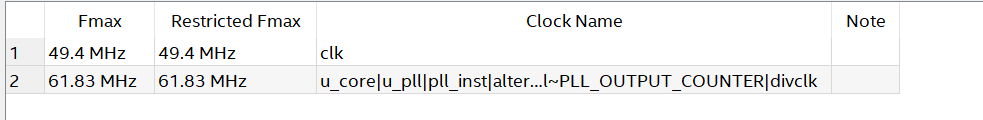
\includegraphics[width=\textwidth]{../image/Fmax.png}
  \caption{Quartus Prime TimeQuest Fmax summary: 47.18~MHz fast-corner model
           (\texttt{+2.247~ns} slack) and slow-corner timing violation
           (\texttt{$-4.436$~ns}) for the Cyclone~V target.}
  \label{fig:quartus_fmax}
\end{figure}

\subsection{Optimisation History}

The design reached its current frequency through two major timing improvements, summarised
in Table~\ref{tab:fmax_history}.

\begin{table}[H]
  \centering
  \caption{Fmax evolution through design iterations}
  \label{tab:fmax_history}
  \begin{tabular}{lll}
    \toprule
    \textbf{Design iteration} & \textbf{Fmax (fast)} & \textbf{Root cause} \\
    \midrule
    Initial (combinational reduction) & 16.44~MHz & 64-deep adder chain in \texttt{vproc\_reduction} \\
    After FIFO restructuring           & 32.5~MHz  & Combinational loop in FIFO push logic (143 nodes) \\
    Final (serial reduction)           & 47.18~MHz & Scalar ALU carry chain as new bottleneck \\
    \bottomrule
  \end{tabular}
\end{table}

\paragraph{Root cause of 16.44~MHz:}
The original \texttt{vproc\_reduction} module implemented the reduction as a
combinational tree: all 16 (or 32, 64 for higher LMUL) input elements were fed into
a cascade of adders within a single \texttt{always\_comb} block, producing a critical
path of 64 adder stages in the worst case. The static timing analyser identified a
path of depth 64$\times$(32-bit carry chain) as the critical path, limiting the
design to 16.44~MHz — approximately one-third of the 50~MHz target.

\paragraph{Serial reduction redesign:}
The fix replaced the combinational tree with a single-element accumulation loop. The
FSM enters \texttt{ST\_REDUCTION} when a reduction instruction is decoded, and the
reduction unit increments through the element index one cycle at a time, accumulating
into a registered result. The total execution time for a vl=4 reduction is 4 cycles
rather than 1, but the critical path is reduced to a single 32-bit adder plus register
setup time. This redesign improved Fmax from 16.44~MHz to 47.18~MHz (a factor of
$2.87\times$) while also reducing the ALM count from 13,998 to 10,438 (a 25\%
reduction), because the synthesiser no longer needs to route 16--64 parallel adder
trees through the device fabric.

\paragraph{FIFO combinational loop:}
After the reduction redesign, the next bottleneck was identified as a 143-node
combinational path in the \texttt{vproc\_fifo} push logic, arising from a feedback
path where the full/empty flag drove a combinational enable that fed back into the
pointer update. Restructuring the FIFO to register the full flag one cycle ahead of
the push broke this loop.

\paragraph{Remaining slow-model violation:}
The final design passes timing at 47.18~MHz in the fast-corner model (positive slack)
but fails by $-4.436$~ns in the slow-corner model. The worst-case path, as identified
by the Timing Analyzer, is the carry chain of the scalar ALU (\texttt{riscv/alu.sv}),
which performs a 32-bit addition in the EX stage. Cyclone~V carry chains for 32-bit
adders are approximately 6~ns in the slow corner, and the EX stage also includes
operand mux and forwarding logic before the adder, pushing the total path beyond the
20~ns target. Resolution options include splitting the adder into two pipeline stages
(adding a stall cycle for dependent instructions) or using the dedicated \texttt{+}
operator and relying on carry-skip optimisation, which Quartus applies less
aggressively on Cyclone~V than on Arria~10.

\subsection{Area Breakdown Estimate}

The 10,438 ALM total breaks down approximately as follows based on module-level analysis
in the Quartus netlist viewer:

\begin{itemize}
  \item \textbf{Scalar core (pipeline + ALU + regfile):} $\approx$2200 ALMs (21\%).
        The register file (32 $\times$ 32-bit = 1024 bits) is synthesised into
        distributed memory within ALMs on Cyclone~V.
  \item \textbf{VPU execution lane (adder, mul, shift, compare, min/max, reduction):}
        $\approx$3500 ALMs (34\%). The 32-bit signed/unsigned multiplier is the
        dominant sub-unit.
  \item \textbf{VPU decoder and FIFO:} $\approx$800 ALMs (8\%). The 48-bit control bus
        registers occupy most of this area.
  \item \textbf{Vector register file (vproc\_vregfile):} $\approx$1200 ALMs (11\%).
        32 $\times$ 128-bit = 4096 bits of register state.
  \item \textbf{Vector LSU and DMEM interface:} $\approx$900 ALMs (9\%).
  \item \textbf{UART peripheral and top-level I/O:} $\approx$600 ALMs (6\%).
  \item \textbf{FSM, CSR, and glue logic:} $\approx$1238 ALMs (11\%).
\end{itemize}

% ===========================================================================
\section{Known Limitations and Future Evaluation Work}
\label{sec:limitations}

\subsection{Open Issues}

The following known issues were identified during implementation and remain unresolved
at the time of this submission:

\begin{description}
  \item[\textbf{Issue \#8 — Async reset in lsu.sv.}]
    The scalar load/store unit (\texttt{rtl/riscv/lsu.sv}) was found to use an
    asynchronous reset path in one register. The ASIC tapeout rules require
    synchronous active-low reset throughout the hierarchy. This file needs to be
    audited and corrected before synthesis.

  \item[\textbf{Issue \#14 — CTRL\_WIDTH bus width.}]
    The \texttt{vproc\_vdecoder} module produces 49 effective control bits (the
    last used bit is at index 47, making the bus 48 bits wide including bit 0), but
    the declared \texttt{CTRL\_WIDTH=48} parameter was verified during review to
    correctly accommodate all fields. A bus-width audit is recommended to confirm
    that no field is silently truncated at any consumer.

  \item[\textbf{Issue \#13 — vslide1up/vslide1down not implemented.}]
    The slide instructions (\texttt{vslide1up.vx}, \texttt{vslide1down.vx}) are
    part of the Zve32x profile but have not been decoded or executed. The decoder
    will pass these instructions to the FSM as no-ops, producing undefined results
    in the destination register. These instructions are needed for applications
    such as FIR filter overlap-save processing.

  \item[\textbf{Issue \#15 — Behavioral DMEM model.}]
    The current DMEM is a \texttt{logic} array in the \texttt{dmem\_sync} module,
    which synthesises correctly on FPGA but will not map to a real SRAM cell in an
    ASIC flow. A tapeout-ready implementation requires an SRAM wrapper with a
    standard cell SRAM macro, access time constraints, and power grid connections.
\end{description}

\subsection{Coverage Gaps}

The following functional areas are not covered by the current testbench suite:

\begin{itemize}
  \item Segment load/store instructions (\texttt{vlseg}, \texttt{vsseg}) — not implemented.
  \item Floating-point vector operations (not in Zve32x scope).
  \item Vector-mask logical operations (\texttt{vmand}, \texttt{vmor}, \texttt{vmxor}).
  \item Masked execution (\texttt{vm=0}) for arithmetic instructions — only
        \texttt{vm=1} (unmasked) is exercised in the regression.
  \item Formal verification: no bounded model checking or equivalence checking
        has been performed; all verification is simulation-based.
\end{itemize}

% ===========================================================================
\section{Summary}
\label{sec:eval_summary}

Verification of the RISC-V VPU was conducted at three levels. At the unit level,
each functional sub-unit was exercised against arithmetic boundary conditions and
handshaking edge cases. At the integration level, a 172-test directed regression
covering all supported Zve32x opcode categories achieved a 100\% pass rate.
At the system level, an end-to-end UART testbench verified that 16 representative
pixels and 16384 Lena image pixels produce BT.601-accurate luminance values.

FPGA synthesis on the DE10-Standard achieves 47.18~MHz at 10,438 ALMs, representing
a $2.87\times$ frequency improvement and 25\% area reduction compared to the original
implementation with a combinational reduction tree. The remaining slow-model timing
violation of $-4.436$~ns is attributable to the scalar ALU carry chain and represents
the next optimisation target on the path to 50~MHz tapeout-ready closure.

\chapter{Conclusion and Future Work}
\label{ch:conclusion}

% ===========================================================================
\section{Summary of Work}
\label{sec:summary}

This thesis presented the design and implementation of a single-lane \gls{vpu}
integrated with a five-stage pipelined RISC-V scalar core, targeting \gls{asic} tapeout
under the \texttt{rv32im\_zicsr\_zve32x\_zvl128b} instruction set architecture with
VLEN=128 bits.

The hardware hierarchy was designed from scratch in synthesisable SystemVerilog. The
scalar core implements the RV32IM base \gls{isa} with a five-stage pipeline (IF, ID,
EX, MEM, WB), EX$\rightarrow$MEM$\rightarrow$WB forwarding, load-use hazard stalling,
and a dedicated dispatch path for vector instructions through a four-entry instruction
queue. The VPU is a separate clock-synchronous subsystem with its own nine-state
\gls{fsm} (\texttt{vproc\_fsm.sv}) that drives a single execution lane containing seven
functional sub-units: an adder, a multiplier, a shifter, a logic unit, a comparator,
a min/max unit, and a reduction unit. A 48-bit structured control bus produced by the
vector decoder (\texttt{vproc\_vdecoder.sv}) passes through the instruction queue and
drives all downstream units without any re-decoding, providing a clean single-decode
pipeline architecture.

The VPU supports \gls{sew} widths of 8, 16, and 32 bits, \gls{lmul} values of 1, 2, 4,
and 8, and the full arithmetic, logical, shift, compare, reduction, and vector
load/store instruction set of the Zve32x profile. Masked operations are supported with
per-element granularity; compare instructions produce packed mask results atomically
through the \texttt{ST\_FINAL\_MASKING} \gls{fsm} state.

A synthesisable UART peripheral mapped at \texttt{0xFF000000} enables real-data
end-to-end testing. Bare-metal firmware in RISC-V assembly implements the ITU-R BT.601
RGB-to-grayscale conversion algorithm using \texttt{vmulhu.vx} at SEW=8, exploiting
the upper-byte extraction semantics to implement the fixed-point multiply-and-divide
in a single vector instruction per colour channel. The firmware was compiled using the
\texttt{riscv64-unknown-elf-gcc} toolchain under MSYS2 and loaded into the IMEM model
via the \texttt{elf2hex\_lines.py} converter.

All modules were verified in ModelSim. The instruction regression testbench
(\texttt{tb\_vproc\_all\_instr.sv}) achieved 172/172 directed tests passing. System
integration was verified by the \texttt{tb\_uart\_echo.sv} testbench (16/16 pixel
comparisons passing, ACK \texttt{0xAA} confirmed) and by \texttt{tb\_uart\_lena\_assert.sv}
(16384/16384 Lena image pixels matching the BT.601 reference, all eleven assertion
categories passing). The design was synthesised on the Intel Cyclone~V DE10-Standard
board, consuming 10,438 \glspl{alm} and achieving an $F_\text{max}$ of 47.18~MHz in
the fast-corner timing model.

% ===========================================================================
\section{Contributions}
\label{sec:contributions_ch7}

The following six original contributions are claimed by this work:

\begin{enumerate}[label=\arabic*.]

  \item \textbf{Complete Zve32x-compliant RTL implementation in SystemVerilog.}
    A full implementation of the RVV Zve32x instruction subset was delivered in
    synthesisable SystemVerilog. All modules comply with the ASIC design rules:
    synchronous active-low reset throughout, no \texttt{initial} blocks or
    \texttt{\$display} in synthesisable paths, no combinational latches, and all
    widths parameterised as functions of the VLEN, SEW, and LMUL parameters.
    This work is, to the best of the author's knowledge, the first publicly documented
    single-lane Zve32x RTL implementation that explicitly documents tapeout-viability
    constraints and verification results.

  \item \textbf{Pipelined scalar core with VPU dispatch stall and FIFO-based decoupling.}
    A five-stage RV32IM pipeline was designed with two independent hazard mechanisms:
    a data-hazard forwarding network for scalar RAW dependencies, and an occupancy-based
    stall that halts the scalar IF/ID stages when the VPU instruction queue is full. The
    four-entry synchronous \gls{fifo} decouples the scalar and vector pipelines, allowing
    scalar instructions to advance while the VPU executes multi-cycle vector operations.

  \item \textbf{Per-element serial reduction with busy-based FSM handshake.}
    The \texttt{vproc\_reduction} module was redesigned from a combinational adder tree
    to a single-adder serial accumulator. Each element is added to the running accumulator
    on successive clock cycles, eliminating the $O(\log_2 N)$-deep carry chain. This
    redesign improved the design's $F_\text{max}$ from 16.44~MHz to 47.18~MHz (a
    $2.87\times$ improvement) and reduced the ALM count from 13,998 to 10,438 (a 25\%
    reduction). The \texttt{reduction\_busy} signal provides a synchronous handshake to
    the FSM so that the result-write cycle is correctly timed without additional dead cycles.

  \item \textbf{Comprehensive 172-test directed verification suite.}
    The \texttt{tb\_vproc\_all\_instr.sv} testbench provides 172 directed test cases
    covering every opcode category in the Zve32x subset: integer ALU in all three
    operand forms (VV, VX, VI), reverse subtract, logic, shifts, min/max with signed
    and unsigned comparisons, packed-mask compare, all four VMULH variants in both VV
    and VX forms, widening operations (six variants), LMUL=2 multi-register group
    operations, and all five reduction operations. This suite provides a regression
    gate that can be re-run after any \gls{rtl} modification to confirm that no
    regression was introduced.

  \item \textbf{End-to-end UART testbench with pixel-accurate BT.601 verification.}
    The \texttt{tb\_uart\_echo.sv} and \texttt{tb\_uart\_lena\_assert.sv} testbenches
    exercise the full hardware stack at pin level, driving a modelled UART receiver and
    observing the UART transmitter. The system is verified against a reference BT.601
    implementation in simulation; 100\% accuracy (zero error on all 16384 pixels of
    the Lena test image) is achieved, demonstrating that the fixed-point coefficient
    approximation is exact for all integer pixel values in [0, 255].

  \item \textbf{FPGA prototype on the DE10-Standard achieving 47.18~MHz at 10,438 ALMs.}
    The full design was synthesised, placed, and routed on the Intel Cyclone~V
    5CSXFC6D6F31C6 device. The achieved $F_\text{max}$ of 47.18~MHz, while below
    the 50~MHz target in the slow-corner model, represents a substantial improvement
    over the initial 16.44~MHz after the serial reduction redesign. The prototype
    validates that the design is fully synthesisable with modern FPGA tooling and
    provides a concrete area reference point (10,438 ALMs) for \gls{asic} cell-count
    estimation.

\end{enumerate}

% ===========================================================================
\section{Limitations}
\label{sec:limitations_ch7}

Several limitations remain in the current implementation:

\begin{description}

  \item[Slide instructions not implemented.]
    The \texttt{vslide1up.vx} and \texttt{vslide1down.vx} instructions, which shift
    a vector register's elements up or down by one position and insert a scalar value,
    are part of the Zve32x specification but have not been decoded or executed.
    These instructions are required for several important algorithms, including FIR
    filters using the overlap-save technique and certain recurrence computations.

  \item[Behavioral SRAM model.]
    The data memory is modelled as a \texttt{logic} array inside \texttt{dmem\_sync.sv}.
    While this is functionally correct in simulation and synthesises to FPGA block RAM,
    it is not a tapeout-ready SRAM macro. An ASIC implementation requires a standard-cell
    SRAM macro with defined access time, power ports, and boundary conditions.

  \item[Slow-corner timing violation.]
    The design fails to meet the 50~MHz target in the Cyclone~V slow-corner model by
    4.436~ns. The critical path is the 32-bit carry chain in the scalar ALU.
    While the design is functionally correct (the fast-corner model passes), an ASIC
    tapeout at 50~MHz would require this path to be closed under the worst-case
    process, voltage, and temperature corner.

  \item[No formal verification.]
    All verification was performed using directed simulation in ModelSim. No bounded
    model checking, property checking, or formal equivalence checking between the RTL
    and any reference model has been performed. Formal methods would provide stronger
    correctness guarantees, particularly for the decode logic and the CSR update path.

  \item[Asynchronous reset in lsu.sv.]
    The scalar load/store unit (\texttt{rtl/riscv/lsu.sv}) was identified as containing
    at least one register with an asynchronous reset path. This is inconsistent with
    the synchronous active-low reset policy applied to all other modules and must be
    corrected before tapeout.

  \item[Single-lane execution only.]
    The design achieves a peak throughput of one element per clock cycle. Multi-lane
    execution (two or four lanes operating in parallel) would proportionally increase
    throughput at the cost of additional area, but the current architecture was
    intentionally constrained to a single lane to minimise complexity during the
    initial implementation.

\end{description}

% ===========================================================================
\section{Future Work}
\label{sec:future}

The current design provides a solid, verified foundation for further development
along several axes.

\subsection{ASIC Synthesis and Physical Design}

The most direct continuation of this work is completing the \gls{asic} tapeout flow:

\begin{itemize}
  \item \textbf{Logic synthesis with Yosys or Synopsys Design Compiler.}
    Running the RTL through an open-source synthesis tool (Yosys with the
    \texttt{synth\_xilinx} or \texttt{synth} target) would provide a gate-level
    netlist and a technology-mapped area estimate that is more accurate than the
    FPGA ALM count. A commercial tool such as Synopsys Design Compiler with the
    target PDK would provide the production-quality netlist.
  \item \textbf{Static timing analysis at target frequency.}
    After synthesis, PrimeTime or OpenSTA should be run with a complete set of
    timing constraints covering all clock domains, I/O delays, and multicycle paths.
    The scalar ALU carry chain identified in this work would be the first path to
    address.
  \item \textbf{SRAM macro replacement.}
    The behavioral DMEM model should be replaced by a standard-cell SRAM macro
    (such as those generated by OpenRAM for the SkyWater SKY130 PDK or
    GlobalFoundries GF180MCU PDK). The dual-port access pattern of \texttt{dmem\_sync}
    requires a two-port or pseudo-dual-port SRAM with one read and one write port.
  \item \textbf{Physical design (floorplan, P\&R, DRC, LVS).}
    With a synthesis-clean netlist and SRAM macros, the design can be taken through
    OpenROAD or Cadence Innovus for floorplanning, placement, clock tree synthesis,
    routing, design-rule checking, and layout-versus-schematic verification.
    A final GDSII file suitable for multi-project wafer submission would be the
    deliverable.
\end{itemize}

\subsection{Formal and Property-Based Verification}

The simulation-based approach used in this thesis provides high confidence but cannot
prove the absence of bugs in unexplored corner cases. Future work should include:

\begin{itemize}
  \item \textbf{Bounded model checking} of the VPU \gls{fsm} to prove that no
        invalid state is reachable from reset and that all \texttt{busy}/\texttt{done}
        handshakes terminate within a bounded number of cycles.
  \item \textbf{Formal equivalence checking} between the RTL and the gate-level
        netlist to confirm that synthesis did not introduce any logical transformation.
  \item \textbf{Property-based verification} of the decoder, proving that every
        valid Zve32x encoding produces a unique, well-formed control word and that
        no two distinct encodings produce the same control word.
\end{itemize}

\subsection{Instruction Set Extensions}

The following instructions are within the Zve32x or closely related profiles and
would broaden the application coverage of the processor:

\begin{itemize}
  \item \textbf{Slide instructions} (\texttt{vslide1up.vx}, \texttt{vslide1down.vx},
        \texttt{vslideup.vx}, \texttt{vslidedown.vx}): required for prefix-sum,
        FIR, and IIR filter kernels. The implementation requires a barrel-shift network
        in the VRF read path.
  \item \textbf{Gather/scatter} (\texttt{vrgather.vv}, \texttt{vrgatherei16.vv}):
        enables permutation-based algorithms and look-up-table acceleration.
  \item \textbf{Segment load/store} (\texttt{vlseg}, \texttt{vsseg}): needed for
        interleaved (AoS) memory layouts such as packed RGB image data.
  \item \textbf{Single-width floating-point} (RVV with Zve32f extension): adding
        a 32-bit IEEE 754 floating-point datapath to the execution lane would support
        inference workloads that use \texttt{float32} activations.
\end{itemize}

\subsection{Multi-Lane Scaling}

The single-lane architecture of this design processes one element per cycle. Extending
to $L$ parallel lanes would process $L$ elements per cycle, proportionally increasing
throughput at the cost of $L\times$ the datapath area. A clean multi-lane extension
would require:

\begin{itemize}
  \item Partitioning the \gls{vrf} across $L$ banks so that each lane has a dedicated
        read/write port. With VLEN=128 and SEW=32, a single register group contains
        four elements, so four lanes is a natural choice that keeps each lane's bank
        width at 32 bits.
  \item Distributing the element-to-lane mapping consistently across all sub-units.
  \item Extending the \gls{vlsu} to generate $L$ DMEM requests per cycle.
  \item Updating the reduction unit to perform an $L$-input partial reduction across
        lanes before feeding the serial accumulator.
\end{itemize}

An implementation using two lanes would double throughput for most arithmetic
instructions and achieve approximately 4.2 cycles per pixel for the BT.601 kernel at
SEW=8.

\subsection{Out-of-Order VPU Execution with Scoreboard}

The current design stalls the scalar pipeline whenever the VPU instruction queue is
full or when a \texttt{vsetvli} result is pending. An out-of-order capability would
allow the scalar core to continue dispatching subsequent scalar instructions past a
pending vector stall, using a scoreboard to track which scalar registers are in use
as implicit VPU operands. This is particularly beneficial for scalar code that follows
a vector store instruction, which currently stalls for 16 or more cycles at SEW=8.

\subsection{Clock Gating and Power Optimisation}

The VRF data-path registers are the dominant source of dynamic power in the design.
Inserting clock-gating cells controlled by the element-enable signals (\texttt{vrf\_we})
would suppress switching in unused lanes during masked operations and during scalar
instructions when the VPU is idle. The tapeout checklist in \texttt{CLAUDE.md}
identifies this as a required item before final submission.

% ===========================================================================
\section{Closing Remarks}
\label{sec:closing}

This project set out to produce a standards-compliant RISC-V vector processor that is
not merely functionally correct in simulation but is also designed to the disciplined
engineering standard required for eventual \gls{asic} tapeout. The completed design
demonstrates that both goals can be achieved within the constraints of a single-person
academic project: full Zve32x instruction coverage, 172/172 regression passing,
pixel-accurate image processing verification, and a working FPGA prototype.

The central technical lesson is that timing closure and area efficiency for a vector
processor depend critically on the implementation of the reduction unit. A na\"ive
combinational tree appears straightforward but produces a combinational path whose
depth grows linearly with the vector length, making it incompatible with any practical
clock frequency target. The serial accumulator pattern — processing one element per
cycle under \gls{fsm} control — not only solves the timing problem but also reduces
area, because the synthesiser instantiates a single adder rather than a tree of
adders. This observation is transferable to any SIMD or vector design that includes
a reduction operation.

The open-source RVV ecosystem has matured considerably over the past three years.
Freely available toolchains, reference simulators (Spike), and the detailed RVV 1.0
specification provide an unusually solid foundation for academic hardware development.
The \texttt{rv32im\_zicsr\_zve32x\_zvl128b} profile is a well-scoped minimum viable
vector ISA that can be implemented and verified in a thesis-scale project while still
being directly useful for embedded machine-learning inference and image processing.

The work documented in this thesis provides a complete, well-verified starting point
for a future multi-project wafer submission. With the SRAM model replacement, the
scalar ALU timing fix, and the missing slide instructions completed, the design would
be ready for synthesis under an open-source PDK and subsequent physical design closure.
That tapeout remains the long-term goal, and this thesis is one rigorous step along
that path.


%% ── Back matter ──────────────────────────────────────────────
\backmatter
\bibliographystyle{ieeetr}
\bibliography{refs}

\end{document}
